\PassOptionsToPackage{unicode=true}{hyperref} % options for packages loaded elsewhere
\PassOptionsToPackage{hyphens}{url}
%
\documentclass[]{book}
\usepackage{lmodern}
\usepackage{amssymb,amsmath}
\usepackage{ifxetex,ifluatex}
\usepackage{fixltx2e} % provides \textsubscript
\ifnum 0\ifxetex 1\fi\ifluatex 1\fi=0 % if pdftex
  \usepackage[T1]{fontenc}
  \usepackage[utf8]{inputenc}
  \usepackage{textcomp} % provides euro and other symbols
\else % if luatex or xelatex
  \usepackage{unicode-math}
  \defaultfontfeatures{Ligatures=TeX,Scale=MatchLowercase}
\fi
% use upquote if available, for straight quotes in verbatim environments
\IfFileExists{upquote.sty}{\usepackage{upquote}}{}
% use microtype if available
\IfFileExists{microtype.sty}{%
\usepackage[]{microtype}
\UseMicrotypeSet[protrusion]{basicmath} % disable protrusion for tt fonts
}{}
\IfFileExists{parskip.sty}{%
\usepackage{parskip}
}{% else
\setlength{\parindent}{0pt}
\setlength{\parskip}{6pt plus 2pt minus 1pt}
}
\usepackage{hyperref}
\hypersetup{
            pdftitle={Visualization, transformation and reporting with the tidyverse},
            pdfauthor={Kirill Müller, Tobias Schieferdecker, Patrick Schratz},
            pdfborder={0 0 0},
            breaklinks=true}
\urlstyle{same}  % don't use monospace font for urls
\usepackage{color}
\usepackage{fancyvrb}
\newcommand{\VerbBar}{|}
\newcommand{\VERB}{\Verb[commandchars=\\\{\}]}
\DefineVerbatimEnvironment{Highlighting}{Verbatim}{commandchars=\\\{\}}
% Add ',fontsize=\small' for more characters per line
\newenvironment{Shaded}{}{}
\newcommand{\AlertTok}[1]{\textcolor[rgb]{1.00,0.00,0.00}{#1}}
\newcommand{\AnnotationTok}[1]{\textcolor[rgb]{0.00,0.50,0.00}{#1}}
\newcommand{\AttributeTok}[1]{#1}
\newcommand{\BaseNTok}[1]{#1}
\newcommand{\BuiltInTok}[1]{#1}
\newcommand{\CharTok}[1]{\textcolor[rgb]{0.00,0.50,0.50}{#1}}
\newcommand{\CommentTok}[1]{\textcolor[rgb]{0.00,0.50,0.00}{#1}}
\newcommand{\CommentVarTok}[1]{\textcolor[rgb]{0.00,0.50,0.00}{#1}}
\newcommand{\ConstantTok}[1]{#1}
\newcommand{\ControlFlowTok}[1]{\textcolor[rgb]{0.00,0.00,1.00}{#1}}
\newcommand{\DataTypeTok}[1]{#1}
\newcommand{\DecValTok}[1]{#1}
\newcommand{\DocumentationTok}[1]{\textcolor[rgb]{0.00,0.50,0.00}{#1}}
\newcommand{\ErrorTok}[1]{\textcolor[rgb]{1.00,0.00,0.00}{\textbf{#1}}}
\newcommand{\ExtensionTok}[1]{#1}
\newcommand{\FloatTok}[1]{#1}
\newcommand{\FunctionTok}[1]{#1}
\newcommand{\ImportTok}[1]{#1}
\newcommand{\InformationTok}[1]{\textcolor[rgb]{0.00,0.50,0.00}{#1}}
\newcommand{\KeywordTok}[1]{\textcolor[rgb]{0.00,0.00,1.00}{#1}}
\newcommand{\NormalTok}[1]{#1}
\newcommand{\OperatorTok}[1]{#1}
\newcommand{\OtherTok}[1]{\textcolor[rgb]{1.00,0.25,0.00}{#1}}
\newcommand{\PreprocessorTok}[1]{\textcolor[rgb]{1.00,0.25,0.00}{#1}}
\newcommand{\RegionMarkerTok}[1]{#1}
\newcommand{\SpecialCharTok}[1]{\textcolor[rgb]{0.00,0.50,0.50}{#1}}
\newcommand{\SpecialStringTok}[1]{\textcolor[rgb]{0.00,0.50,0.50}{#1}}
\newcommand{\StringTok}[1]{\textcolor[rgb]{0.00,0.50,0.50}{#1}}
\newcommand{\VariableTok}[1]{#1}
\newcommand{\VerbatimStringTok}[1]{\textcolor[rgb]{0.00,0.50,0.50}{#1}}
\newcommand{\WarningTok}[1]{\textcolor[rgb]{0.00,0.50,0.00}{\textbf{#1}}}
\usepackage{longtable,booktabs}
% Fix footnotes in tables (requires footnote package)
\IfFileExists{footnote.sty}{\usepackage{footnote}\makesavenoteenv{longtable}}{}
\usepackage{graphicx,grffile}
\makeatletter
\def\maxwidth{\ifdim\Gin@nat@width>\linewidth\linewidth\else\Gin@nat@width\fi}
\def\maxheight{\ifdim\Gin@nat@height>\textheight\textheight\else\Gin@nat@height\fi}
\makeatother
% Scale images if necessary, so that they will not overflow the page
% margins by default, and it is still possible to overwrite the defaults
% using explicit options in \includegraphics[width, height, ...]{}
\setkeys{Gin}{width=\maxwidth,height=\maxheight,keepaspectratio}
\setlength{\emergencystretch}{3em}  % prevent overfull lines
\providecommand{\tightlist}{%
  \setlength{\itemsep}{0pt}\setlength{\parskip}{0pt}}
\setcounter{secnumdepth}{5}
% Redefines (sub)paragraphs to behave more like sections
\ifx\paragraph\undefined\else
\let\oldparagraph\paragraph
\renewcommand{\paragraph}[1]{\oldparagraph{#1}\mbox{}}
\fi
\ifx\subparagraph\undefined\else
\let\oldsubparagraph\subparagraph
\renewcommand{\subparagraph}[1]{\oldsubparagraph{#1}\mbox{}}
\fi

% set default figure placement to htbp
\makeatletter
\def\fps@figure{htbp}
\makeatother

\usepackage{etoolbox}
\makeatletter
\providecommand{\subtitle}[1]{% add subtitle to \maketitle
  \apptocmd{\@title}{\par {\large #1 \par}}{}{}
}
\makeatother
\usepackage{booktabs}
% https://github.com/rstudio/rmarkdown/issues/337
\let\rmarkdownfootnote\footnote%
\def\footnote{\protect\rmarkdownfootnote}

% https://github.com/rstudio/rmarkdown/pull/252
\usepackage{titling}
\setlength{\droptitle}{-2em}

\pretitle{\vspace{\droptitle}\centering\huge}
\posttitle{\par}

\preauthor{\centering\large\emph}
\postauthor{\par}

\predate{\centering\large\emph}
\postdate{\par}
\usepackage[]{natbib}
\bibliographystyle{apa-old.cls}

\title{Visualization, transformation and reporting with the tidyverse}
\author{Kirill Müller, Tobias Schieferdecker, Patrick Schratz}
\date{28 November 2019, 00:03 CET}

\begin{document}
\maketitle

{
\setcounter{tocdepth}{1}
\tableofcontents
}
\hypertarget{preface}{%
\chapter*{Preface}\label{preface}}
\addcontentsline{toc}{chapter}{Preface}

See the controls at the top of the website for searching, font size, editing, and a link to the PDF version of the material.

\hypertarget{links}{%
\section*{Links}\label{links}}
\addcontentsline{toc}{section}{Links}

\begin{itemize}
\item
  This website: \url{https://krlmlr.github.io/vistransrep}
\item
  Scripts and installation instructions: \url{https://github.com/krlmlr/vistransrep-proj/tree/master}

  \begin{itemize}
  \tightlist
  \item
    Prepared scripts: \url{https://github.com/krlmlr/vistransrep-proj/tree/master/script}
  \end{itemize}
\item
  The source project for this material: \url{https://github.com/krlmlr/vistransrep}
\end{itemize}

\hypertarget{download-data-and-code}{%
\section*{Download data and code}\label{download-data-and-code}}
\addcontentsline{toc}{section}{Download data and code}

\begin{Shaded}
\begin{Highlighting}[]
\NormalTok{usethis}\OperatorTok{::}\KeywordTok{use_course}\NormalTok{(}\StringTok{"krlmlr/vistransrep-proj"}\NormalTok{)}
\end{Highlighting}
\end{Shaded}

\hypertarget{package-versions-used}{%
\section*{Package versions used}\label{package-versions-used}}
\addcontentsline{toc}{section}{Package versions used}

Click to expand

\begin{Shaded}
\begin{Highlighting}[]
\NormalTok{withr}\OperatorTok{::}\KeywordTok{with_options}\NormalTok{(}\KeywordTok{list}\NormalTok{(}\DataTypeTok{width =} \DecValTok{80}\NormalTok{), }\KeywordTok{print}\NormalTok{(sessioninfo}\OperatorTok{::}\KeywordTok{session_info}\NormalTok{()))}
\end{Highlighting}
\end{Shaded}

\begin{verbatim}
## - Session info ---------------------------------------------------------------
##  setting  value                       
##  version  R version 3.6.1 (2017-01-27)
##  os       Ubuntu 16.04.6 LTS          
##  system   x86_64, linux-gnu           
##  ui       X11                         
##  language en_US.UTF-8                 
##  collate  en_US.UTF-8                 
##  ctype    en_US.UTF-8                 
##  tz       UTC                         
##  date     2019-11-27                  
## 
## - Packages -------------------------------------------------------------------
##  package      * version     date       lib source                           
##  askpass        1.1         2019-01-13 [1] CRAN (R 3.6.1)                   
##  assertthat     0.2.1       2019-03-21 [1] CRAN (R 3.6.1)                   
##  backports      1.1.5       2019-10-02 [1] CRAN (R 3.6.1)                   
##  bookdown       0.16        2019-11-22 [1] CRAN (R 3.6.1)                   
##  broom          0.5.2       2019-04-07 [1] CRAN (R 3.6.1)                   
##  cellranger     1.1.0       2016-07-27 [1] CRAN (R 3.6.1)                   
##  cli            1.1.0       2019-03-19 [1] CRAN (R 3.6.1)                   
##  codetools      0.2-16      2018-12-24 [3] CRAN (R 3.6.1)                   
##  colorspace     1.4-1       2019-03-18 [1] CRAN (R 3.6.1)                   
##  crayon         1.3.4       2017-09-16 [1] CRAN (R 3.6.1)                   
##  crosstalk      1.0.0       2016-12-21 [1] CRAN (R 3.6.1)                   
##  data.table     1.12.6      2019-10-18 [1] CRAN (R 3.6.1)                   
##  DBI            1.0.0       2018-05-02 [1] CRAN (R 3.6.1)                   
##  dbplyr         1.4.2       2019-06-17 [1] CRAN (R 3.6.1)                   
##  digest         0.6.23      2019-11-23 [1] CRAN (R 3.6.1)                   
##  dplyr        * 0.8.3       2019-07-04 [1] CRAN (R 3.6.1)                   
##  DT             0.10        2019-11-12 [1] CRAN (R 3.6.1)                   
##  ellipsis       0.3.0       2019-09-20 [1] CRAN (R 3.6.1)                   
##  evaluate       0.14        2019-05-28 [1] CRAN (R 3.6.1)                   
##  fansi          0.4.0       2018-10-05 [1] CRAN (R 3.6.1)                   
##  farver         2.0.1       2019-11-13 [1] CRAN (R 3.6.1)                   
##  fastmap        1.0.1       2019-10-08 [1] CRAN (R 3.6.1)                   
##  forcats      * 0.4.0       2019-02-17 [1] CRAN (R 3.6.1)                   
##  fs             1.3.1       2019-05-06 [1] CRAN (R 3.6.1)                   
##  generics       0.0.2       2018-11-29 [1] CRAN (R 3.6.1)                   
##  ggplot2      * 3.2.1       2019-08-10 [1] CRAN (R 3.6.1)                   
##  ggpubr         0.2.4       2019-11-14 [1] CRAN (R 3.6.1)                   
##  ggsignif       0.6.0       2019-08-08 [1] CRAN (R 3.6.1)                   
##  git2r          0.26.1      2019-06-29 [1] CRAN (R 3.6.1)                   
##  glue           1.3.1       2019-03-12 [1] CRAN (R 3.6.1)                   
##  gtable         0.3.0       2019-03-25 [1] CRAN (R 3.6.1)                   
##  haven          2.2.0       2019-11-08 [1] CRAN (R 3.6.1)                   
##  here         * 0.1         2017-05-28 [1] CRAN (R 3.6.1)                   
##  hms            0.5.2       2019-10-30 [1] CRAN (R 3.6.1)                   
##  htmltools      0.4.0       2019-10-04 [1] CRAN (R 3.6.1)                   
##  htmlwidgets    1.5.1       2019-10-08 [1] CRAN (R 3.6.1)                   
##  httpuv         1.5.2       2019-09-11 [1] CRAN (R 3.6.1)                   
##  httr           1.4.1       2019-08-05 [1] CRAN (R 3.6.1)                   
##  jsonlite       1.6         2018-12-07 [1] CRAN (R 3.6.1)                   
##  knitr          1.26        2019-11-12 [1] CRAN (R 3.6.1)                   
##  labeling       0.3         2014-08-23 [1] CRAN (R 3.6.1)                   
##  later          1.0.0       2019-10-04 [1] CRAN (R 3.6.1)                   
##  lattice        0.20-38     2018-11-04 [3] CRAN (R 3.6.1)                   
##  lazyeval       0.2.2       2019-03-15 [1] CRAN (R 3.6.1)                   
##  leaflet      * 2.0.3       2019-11-16 [1] CRAN (R 3.6.1)                   
##  lifecycle      0.1.0       2019-08-01 [1] CRAN (R 3.6.1)                   
##  lubridate      1.7.4       2018-04-11 [1] CRAN (R 3.6.1)                   
##  magrittr       1.5         2014-11-22 [1] CRAN (R 3.6.1)                   
##  MASS           7.3-51.4    2019-03-31 [3] CRAN (R 3.6.1)                   
##  memoise        1.1.0       2017-04-21 [1] CRAN (R 3.6.1)                   
##  mime           0.7         2019-06-11 [1] CRAN (R 3.6.1)                   
##  modelr         0.1.5       2019-08-08 [1] CRAN (R 3.6.1)                   
##  munsell        0.5.0       2018-06-12 [1] CRAN (R 3.6.1)                   
##  nlme           3.1-140     2019-05-12 [3] CRAN (R 3.6.1)                   
##  nycflights13 * 1.0.1       2019-09-16 [1] CRAN (R 3.6.1)                   
##  openssl        1.4.1       2019-07-18 [1] CRAN (R 3.6.1)                   
##  pillar         1.4.2       2019-06-29 [1] CRAN (R 3.6.1)                   
##  pkgconfig      2.0.3       2019-09-22 [1] CRAN (R 3.6.1)                   
##  plotly         4.9.1       2019-11-07 [1] CRAN (R 3.6.1)                   
##  plyr           1.8.4       2016-06-08 [1] CRAN (R 3.6.1)                   
##  promises       1.1.0       2019-10-04 [1] CRAN (R 3.6.1)                   
##  purrr        * 0.3.3       2019-10-18 [1] CRAN (R 3.6.1)                   
##  R6             2.4.1       2019-11-12 [1] CRAN (R 3.6.1)                   
##  RColorBrewer   1.1-2       2014-12-07 [1] CRAN (R 3.6.1)                   
##  Rcpp           1.0.3       2019-11-08 [1] CRAN (R 3.6.1)                   
##  readr        * 1.3.1       2018-12-21 [1] CRAN (R 3.6.1)                   
##  readxl         1.3.1       2019-03-13 [1] CRAN (R 3.6.1)                   
##  reprex         0.3.0       2019-05-16 [1] CRAN (R 3.6.1)                   
##  reshape2       1.4.3       2017-12-11 [1] CRAN (R 3.6.1)                   
##  rlang          0.4.2.9000  2019-11-27 [1] Github (r-lib/rlang@1be25e7)     
##  rmarkdown      1.18        2019-11-27 [1] CRAN (R 3.6.1)                   
##  rprojroot      1.3-2       2018-01-03 [1] CRAN (R 3.6.1)                   
##  rstudioapi     0.10        2019-03-19 [1] CRAN (R 3.6.1)                   
##  rvest          0.3.5       2019-11-08 [1] CRAN (R 3.6.1)                   
##  scales         1.1.0       2019-11-18 [1] CRAN (R 3.6.1)                   
##  sessioninfo    1.1.1       2018-11-05 [1] CRAN (R 3.6.1)                   
##  shiny          1.4.0       2019-10-10 [1] CRAN (R 3.6.1)                   
##  stringi        1.4.3       2019-03-12 [1] CRAN (R 3.6.1)                   
##  stringr      * 1.4.0       2019-02-10 [1] CRAN (R 3.6.1)                   
##  tibble       * 2.1.3       2019-06-06 [1] CRAN (R 3.6.1)                   
##  tic            0.2.13.9021 2019-11-27 [1] Github (ropenscilabs/tic@8d76ddb)
##  tidyr        * 1.0.0       2019-09-11 [1] CRAN (R 3.6.1)                   
##  tidyselect     0.2.5       2018-10-11 [1] CRAN (R 3.6.1)                   
##  tidyverse    * 1.3.0       2019-11-21 [1] CRAN (R 3.6.1)                   
##  utf8           1.1.4       2018-05-24 [1] CRAN (R 3.6.1)                   
##  vctrs          0.2.0       2019-07-05 [1] CRAN (R 3.6.1)                   
##  viridisLite    0.3.0       2018-02-01 [1] CRAN (R 3.6.1)                   
##  withr          2.1.2       2018-03-15 [1] CRAN (R 3.6.1)                   
##  xaringan       0.13        2019-10-30 [1] CRAN (R 3.6.1)                   
##  xfun           0.11        2019-11-12 [1] CRAN (R 3.6.1)                   
##  xml2           1.2.2       2019-08-09 [1] CRAN (R 3.6.1)                   
##  xtable         1.8-4       2019-04-21 [1] CRAN (R 3.6.1)                   
##  yaml           2.2.0       2018-07-25 [1] CRAN (R 3.6.1)                   
##  zeallot        0.1.0       2018-01-28 [1] CRAN (R 3.6.1)                   
## 
## [1] /home/travis/R/Library
## [2] /usr/local/lib/R/site-library
## [3] /home/travis/R-bin/lib/R/library
\end{verbatim}

\hypertarget{license}{%
\section*{License}\label{license}}
\addcontentsline{toc}{section}{License}

Licensed under \href{https://creativecommons.org/licenses/by-nc/4.0/}{CC-BY-NC 4.0}.

\hypertarget{speakers}{%
\section*{Speakers}\label{speakers}}
\addcontentsline{toc}{section}{Speakers}

\textbf{Kirill Müller} (@krlmlr) \url{https://www.cynkra.com/about.html}

\begin{flushright}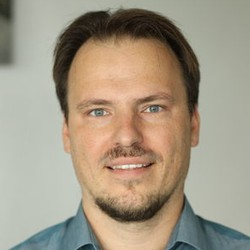
\includegraphics[width=3.47in]{img/kirill} \end{flushright}

\begin{itemize}
\tightlist
\item
  Co-founder cynkra
\item
  Computer + data science
\item
  Workflows, user interfaces, databases
\item
  R package author + maintainer
\end{itemize}

\textbf{Patrick Schratz} (@pat-s) \url{https://pat-s.me}

\begin{flushright}
\includegraphics[width=3.47in]{img/pjs} \end{flushright}

\begin{itemize}
\tightlist
\item
  M.Sc. Geoinformatics
\item
  Researcher/Research Engineer at University of \textbf{Jena} and \textbf{LMU Munich}
\item
  PhD Candidate
\end{itemize}

\begin{center}\rule{0.5\linewidth}{\linethickness}\end{center}

\begin{itemize}
\tightlist
\item
  Unix \& R enthusiast
\item
  Author/Contributor/Maintainer of several R packages:

  \begin{itemize}
  \tightlist
  \item
    (\href{https://github.com/mlr-org/mlr3}{mlr3}, \href{https://github.com/mlr-org/mlr}{mlr})
  \item
    sperrorest
  \item
    oddsratio
  \item
    xaringan
  \item
    circle
  \item
    RQGIS
  \item
    travis
  \item
    tic
  \item
    \ldots{}
  \end{itemize}
\end{itemize}

\hypertarget{introduction}{%
\section*{Introduction}\label{introduction}}
\addcontentsline{toc}{section}{Introduction}

\begin{figure}

\hfill{}
\includegraphics[width=11.11in]{img/r_first_then} 

\caption{© Allison Horst}\label{fig:r-first}
\end{figure}

The \texttt{tidyverse} has quickly developed over the last years.
Its first implementation as a collection of partly older packages was in the second half of 2016.
All its packages ``share an underlying design philosophy, grammar, and data structures.''\footnote{citation from \href{https://www.tidyverse.org/}{tidyverse homepage}}
It is for sure difficult to tell, if ``learning the \texttt{tidyverse}'' is a hard task, since the result of this assessment might differ from person to person.
We do believe though, that there are concepts in its approach, which -- when grasped -- have the potential to increase one's productivity, since code creation will seem more natural.
While this might be true for all languages (once you speak it well enough, things go smoothly), in our opinion the \texttt{tidyverse} worth exploring in depth, since it is

\begin{enumerate}
\def\labelenumi{\arabic{enumi}.}
\tightlist
\item
  consistent: an especially well designed framework that aims at making data analysis and programming intuitive,
\item
  evolving: constantly deepened understanding for challenges arising in modern data analysis leads to improving ergonomic user interfaces.
\end{enumerate}

This course covers several topics, which everyone working more intently with the \texttt{tidyverse} almost inevitably needs to deal with at some point or another.
The topics are organized in chapters that contain mostly R code with output and text.
In each section, exercises are provided.

\begin{Shaded}
\begin{Highlighting}[]
\NormalTok{knitr}\OperatorTok{::}\KeywordTok{include_graphics}\NormalTok{(}\StringTok{"img/environmental-data-science-r4ds-general.png"}\NormalTok{)}
\end{Highlighting}
\end{Shaded}

\hypertarget{r-and-rstudio}{%
\chapter{R and RStudio}\label{r-and-rstudio}}

\hypertarget{r-as-a-toolkit}{%
\section{R as a toolkit}\label{r-as-a-toolkit}}

\begin{figure}
\centering

\includegraphics{img/toolkit.png}
\caption{R as a toolkit}
\end{figure}

\begin{itemize}
\tightlist
\item
  Scriptability \(\rightarrow\) R
\item
  Literate programming (code, narrative, output in one place) \(\rightarrow\) R Markdown
\item
  Version control \(\rightarrow\) Git / GitHub
\end{itemize}

\hypertarget{why-r-and-rstudio}{%
\subsection{Why R and RStudio?}\label{why-r-and-rstudio}}

\begin{flushright}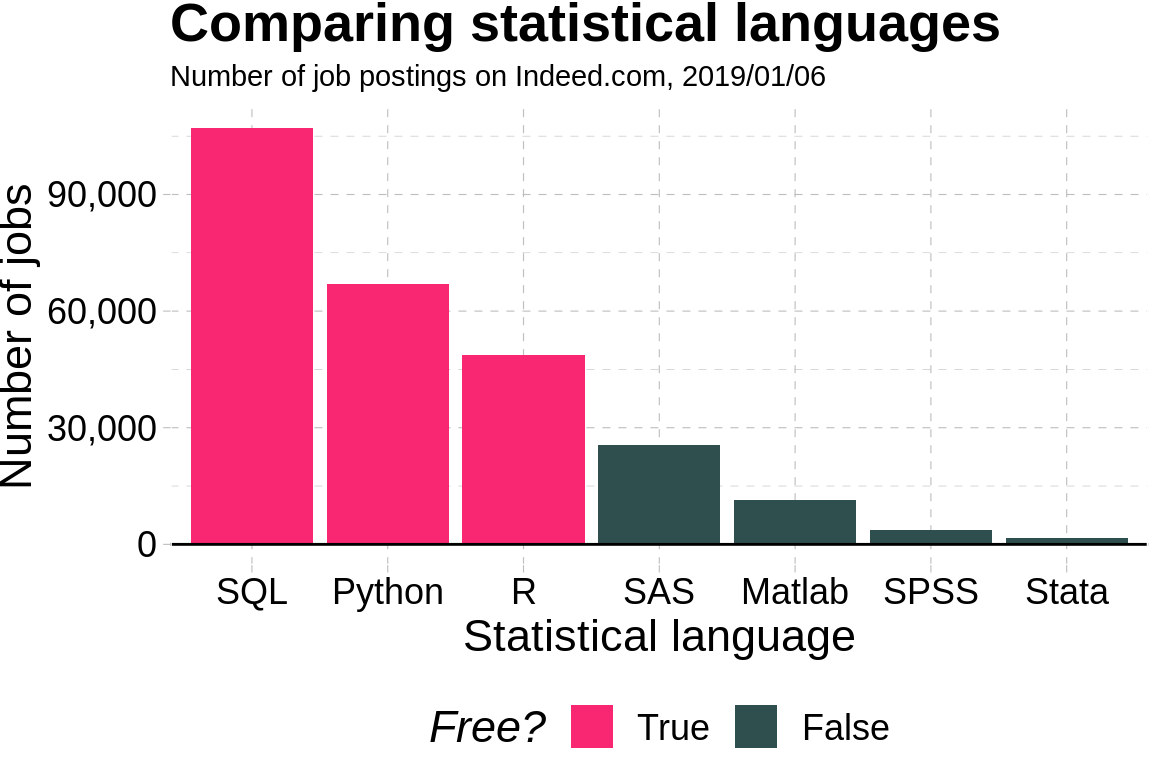
\includegraphics{vistransrep_files/figure-latex/indeeddotcom-1} \end{flushright}

\hypertarget{some-r-basics}{%
\subsection{Some R basics}\label{some-r-basics}}

\begin{itemize}
\tightlist
\item
  You will load packages at the \textbf{start of every new R session}.

  \begin{itemize}
  \tightlist
  \item
    ``Base'' R comes with tons of useful built-in functions. It also provides all the tools necessary for you to write your own functions.
  \item
    However, many of R's best data science functions and tools come from external packages written by other users.
  \end{itemize}
\item
  R easily and infinitely parallelizes. For free.

  \begin{itemize}
  \tightlist
  \item
    Compare the cost of a \href{https://www.stata.com/statamp/}{Stata/MP} license, nevermind the fact that you effectively pay per core\ldots{}
  \end{itemize}
\end{itemize}

\hypertarget{r-code-examples}{%
\section{R code examples}\label{r-code-examples}}

\hypertarget{linear-regression}{%
\subsection{Linear regression}\label{linear-regression}}

\begin{Shaded}
\begin{Highlighting}[]
\NormalTok{fit <-}\StringTok{ }\KeywordTok{lm}\NormalTok{(dist }\OperatorTok{~}\StringTok{ }\DecValTok{1} \OperatorTok{+}\StringTok{ }\NormalTok{speed, }\DataTypeTok{data =}\NormalTok{ cars)}
\KeywordTok{summary}\NormalTok{(fit)}
\end{Highlighting}
\end{Shaded}

\begin{verbatim}
## 
## Call:
## lm(formula = dist ~ 1 + speed, data = cars)
## 
## Residuals:
##     Min      1Q  Median      3Q     Max 
## -29.069  -9.525  -2.272   9.215  43.201 
## 
## Coefficients:
##             Estimate Std. Error t value Pr(>|t|)    
## (Intercept) -17.5791     6.7584  -2.601   0.0123 *  
## speed         3.9324     0.4155   9.464 1.49e-12 ***
## ---
## Signif. codes:  0 '***' 0.001 '**' 0.01 '*' 0.05 '.' 0.1 ' ' 1
## 
## Residual standard error: 15.38 on 48 degrees of freedom
## Multiple R-squared:  0.6511, Adjusted R-squared:  0.6438 
## F-statistic: 89.57 on 1 and 48 DF,  p-value: 1.49e-12
\end{verbatim}

\hypertarget{base-r-plot}{%
\subsection{Base R plot}\label{base-r-plot}}

\begin{Shaded}
\begin{Highlighting}[]
\KeywordTok{plot}\NormalTok{(cars, }\DataTypeTok{pch =} \DecValTok{19}\NormalTok{, }\DataTypeTok{col =} \StringTok{"darkgray"}\NormalTok{)}
\KeywordTok{abline}\NormalTok{(fit, }\DataTypeTok{lwd =} \DecValTok{2}\NormalTok{)}
\end{Highlighting}
\end{Shaded}

\begin{flushright}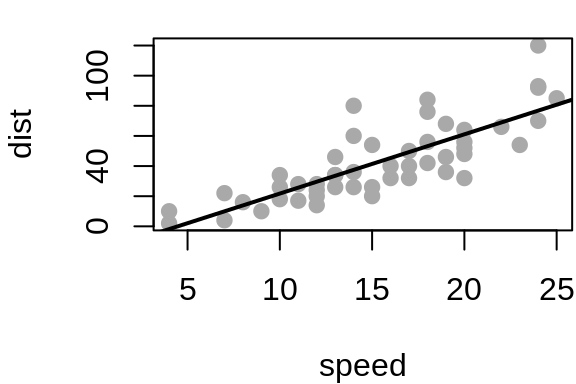
\includegraphics{vistransrep_files/figure-latex/cars_basefig-1} \end{flushright}

\hypertarget{ggplot2}{%
\subsection{ggplot2}\label{ggplot2}}

\begin{Shaded}
\begin{Highlighting}[]
\KeywordTok{library}\NormalTok{(ggplot2)}
\KeywordTok{library}\NormalTok{(gapminder) ## For the gapminder data}

\KeywordTok{ggplot}\NormalTok{(}
  \DataTypeTok{data =}\NormalTok{ gapminder,}
  \DataTypeTok{mapping =} \KeywordTok{aes}\NormalTok{(}\DataTypeTok{x =}\NormalTok{ gdpPercap, }\DataTypeTok{y =}\NormalTok{ lifeExp)}
\NormalTok{) }\OperatorTok{+}
\StringTok{  }\KeywordTok{geom_point}\NormalTok{()}
\end{Highlighting}
\end{Shaded}

\begin{flushright}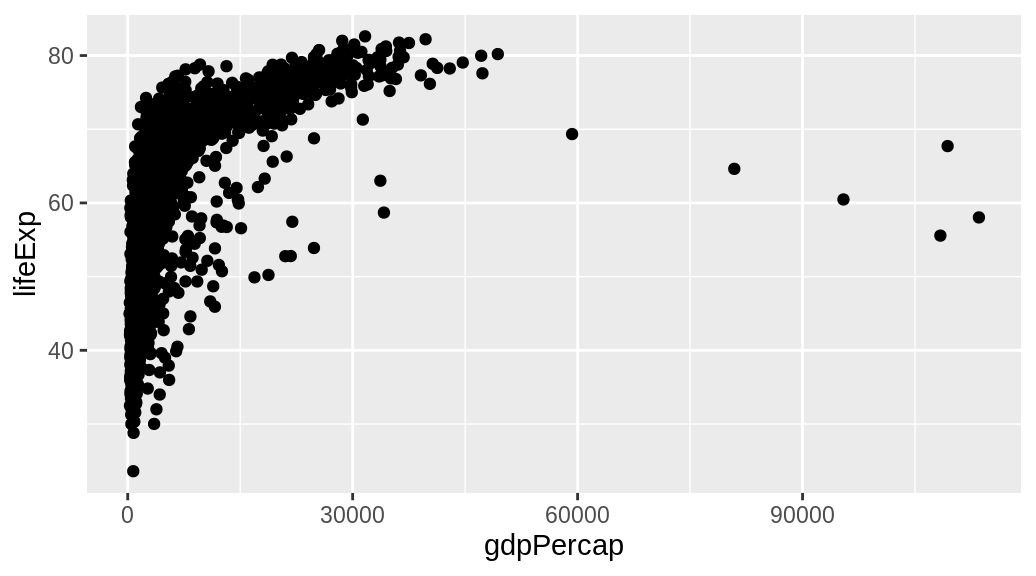
\includegraphics{vistransrep_files/figure-latex/gapm_plot-1} \end{flushright}

\hypertarget{gganimate}{%
\subsection{gganimate}\label{gganimate}}

\hypertarget{r-vs.rstudio}{%
\section{R vs.~RStudio}\label{r-vs.rstudio}}

\begin{itemize}
\tightlist
\item
  R is a statistical \textbf{programming language}
\item
  RStudio is a convenient interface for R (an \textbf{integrated development environment}, IDE)
\item
  At its simplest:

  \begin{itemize}
  \tightlist
  \item
    R is like a car's engine
  \item
    RStudio is like a car's dashboard
  \end{itemize}
\end{itemize}

\begin{figure}
\centering
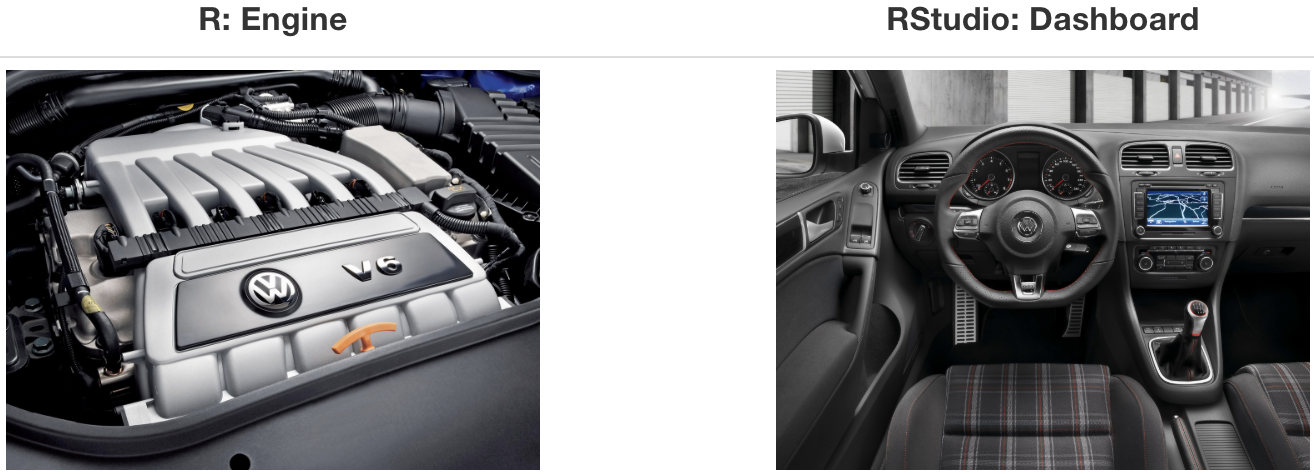
\includegraphics{img/engine-dashboard.png}
\caption{Engine vs.~dashboard}
\end{figure}

\hypertarget{r-vs.r-packages}{%
\section{R vs.~R packages}\label{r-vs.r-packages}}

\begin{itemize}
\item
  R packages \textbf{extend} the functionality of R by providing additional functions, data, and documentation.
\item
  They are written by a world-wide community of R users and can be downloaded for no cost
\end{itemize}

\begin{figure}
\centering
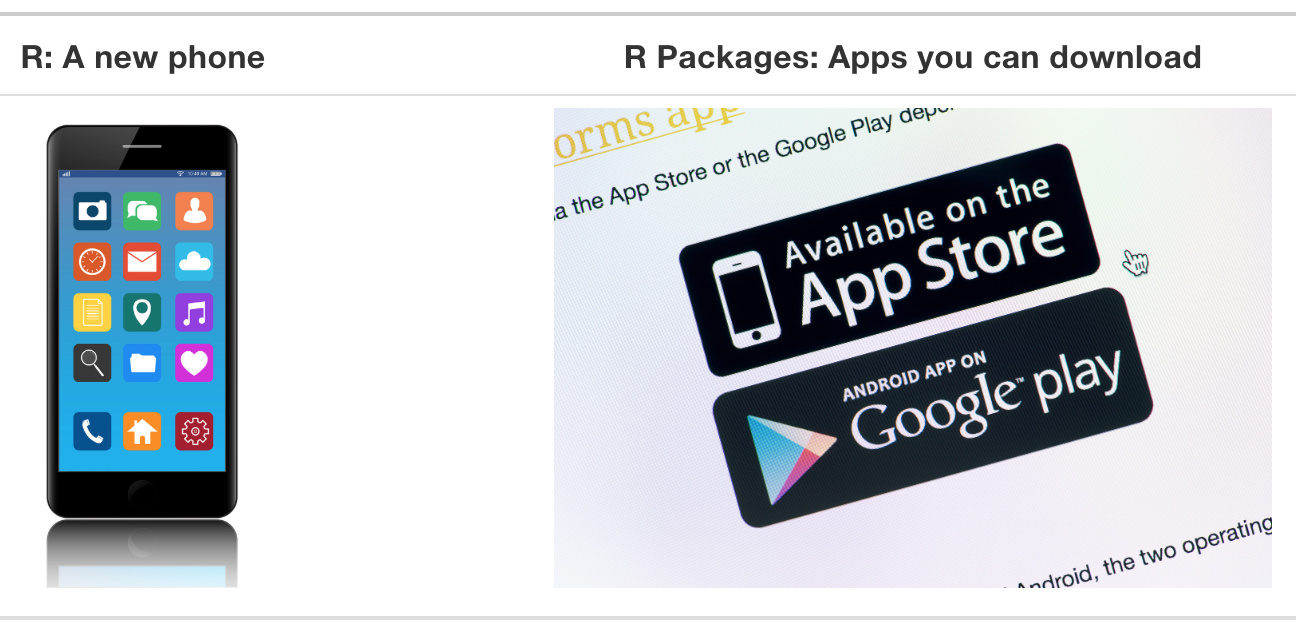
\includegraphics{img/r_vs_r_packages.png}
\caption{R versus R packages}
\end{figure}

\hypertarget{r-packages}{%
\section{R packages}\label{r-packages}}

\begin{itemize}
\item
  \textbf{CRAN}: A group of people who check that packages fulfill certain standards
\item
  \textbf{Mirror}: A location on the web where to download R packages from. Because many thousand people download them daily, the load is distributed on different machines. Pick one which is geographically close to you
\item
  \textbf{R base/recommended packages}: The base installation of R ships with a bunch of default packages. In addition, there are some more packages listed as ``recommended''.
\end{itemize}

``base'' packages are managed by the R core team and will only be updated for every R release.

Packages listed as ``recommended'' inherit the attributes of being widely used and having a long history in the R community.

\begin{verbatim}
##     Package Priority
## 1      base     base
## 2  compiler     base
## 3  datasets     base
## 4  graphics     base
## 5 grDevices     base
## 6      grid     base
## 7   methods     base
## 8  parallel     base
\end{verbatim}

\begin{verbatim}
##       Package    Priority
## 1        boot recommended
## 2       class recommended
## 3     cluster recommended
## 4   codetools recommended
## 5     foreign recommended
## 6  KernSmooth recommended
## 7     lattice recommended
## 8        MASS recommended
## 9      Matrix recommended
## 10       mgcv recommended
##  [ reached 'max' / getOption("max.print") -- omitted 2 rows ]
\end{verbatim}

\hypertarget{rprofile}{%
\section{.Rprofile}\label{rprofile}}

\begin{itemize}
\item
  File in your home directory \texttt{\textasciitilde{}/.Rprofile}
\item
  Will be executed before every R session starts
\item
  Useful to set global options and for loading of often used packages
\end{itemize}

\hypertarget{renviron}{%
\section{.Renviron}\label{renviron}}

\begin{itemize}
\item
  File in your home directory \texttt{\textasciitilde{}/.Renviron}
\item
  Used to set environment variables
\item
  Used to store ``Access tokens'' (Github, CI provider, C++ flags)
\end{itemize}

\hypertarget{rstudio}{%
\section{RStudio}\label{rstudio}}

\(\rightarrow\) Exists to \textbf{boost} your productivity

\(\rightarrow\) Change the defaults to your liking so you \emph{actually} can be \textbf{productive}

\(\rightarrow\) Keybindings = productivity

Since RStudio v1.3 a \href{https://docs.rstudio.com/ide/desktop-pro/latest/settings.html\#preferences}{portable JSON settings file} exists.

If you want to have sane settings without much hassle, you can execute the following R code: \texttt{source("https://bit.ly/rstudio-pat")}

This code will change/overwrite your existing RStudio settings and

\begin{itemize}
\item
  set custom keybindings
\item
  move the console panel to the top-right (by default bottom-left)
\item
  Enable/Disable some core settings to have a better overall experience
\end{itemize}

\begin{center}\rule{0.5\linewidth}{\linethickness}\end{center}

R scripts (source code) are written in the \emph{Source} pane (Editor).

\begin{figure}
\centering
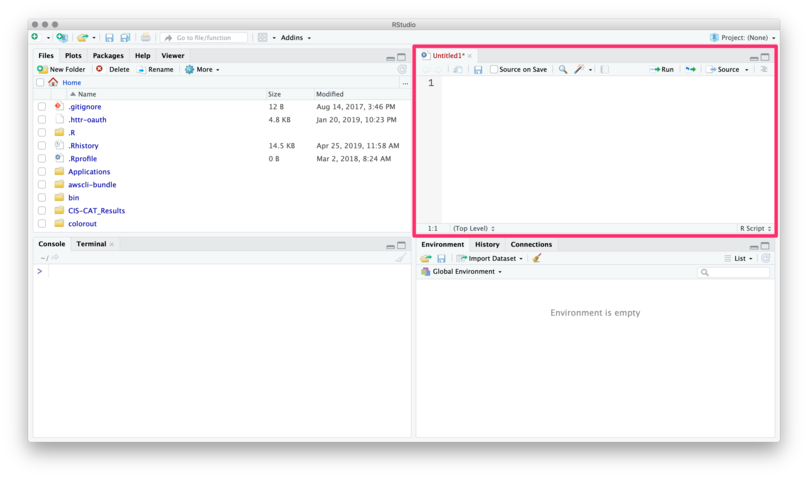
\includegraphics{img/rstudio_source_rec.png}
\caption{Source pane}
\end{figure}

(Source of all following RStudio screenshots: \url{https://github.com/edrubin/EC525S19})

\begin{center}\rule{0.5\linewidth}{\linethickness}\end{center}

You can use the menubar or ⇧+⌘+N / ⇧+CTRL+N to create new R scripts.

\begin{figure}
\centering
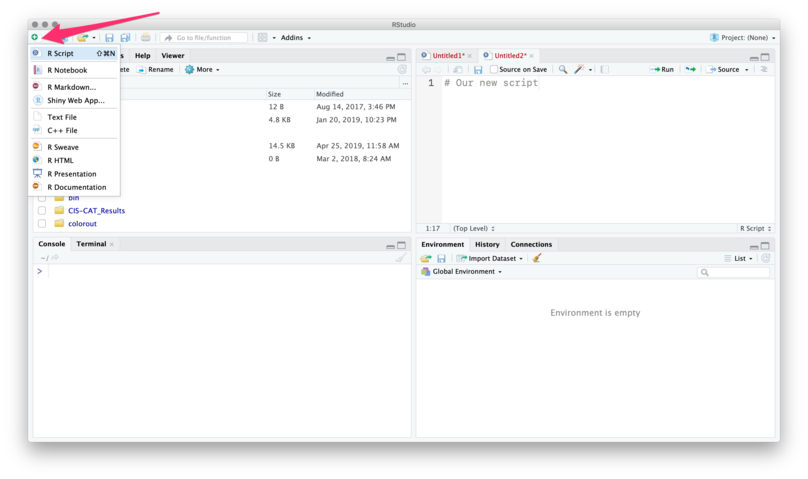
\includegraphics{img/rstudio_source_arrow.png}
\caption{New script}
\end{figure}

\begin{center}\rule{0.5\linewidth}{\linethickness}\end{center}

To execute commands from your R script, use ⌘+Enter / CTRL+Enter.

\begin{figure}
\centering
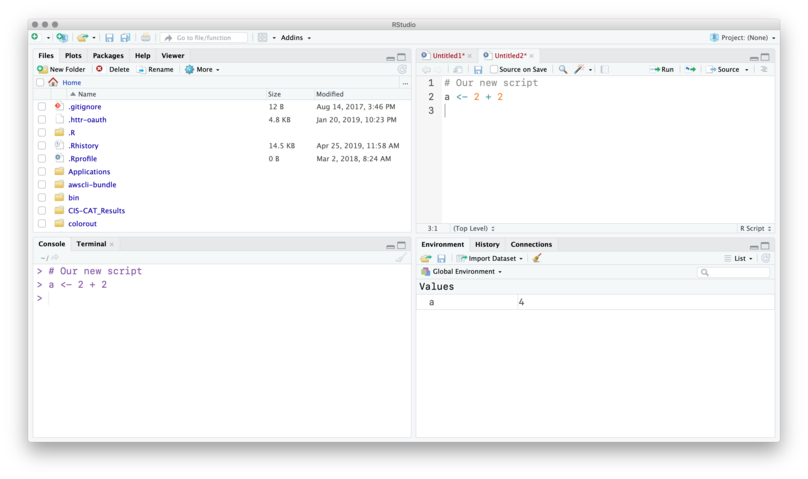
\includegraphics{img/rstudio_source_ex.png}
\caption{Execute commands}
\end{figure}

RStudio will execute the command in the console.

\begin{figure}
\centering
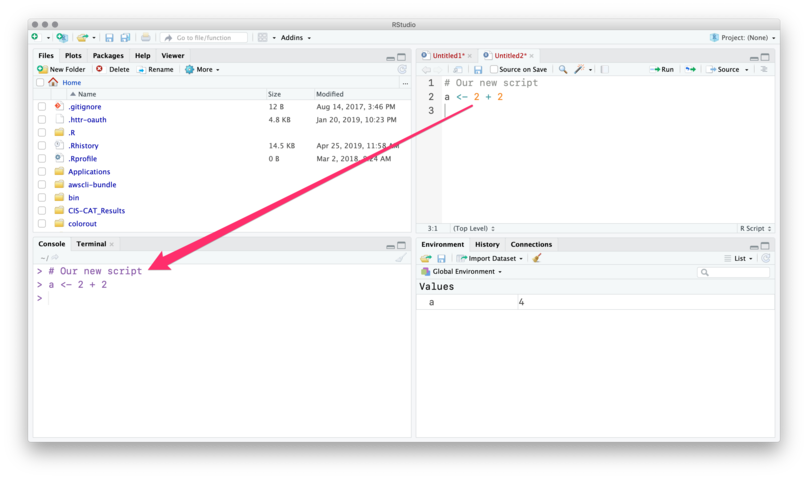
\includegraphics{img/rstudio_source_ex2.png}
\caption{Console output}
\end{figure}

You can see the new object in the \emph{Environment} pane.

\begin{figure}
\centering
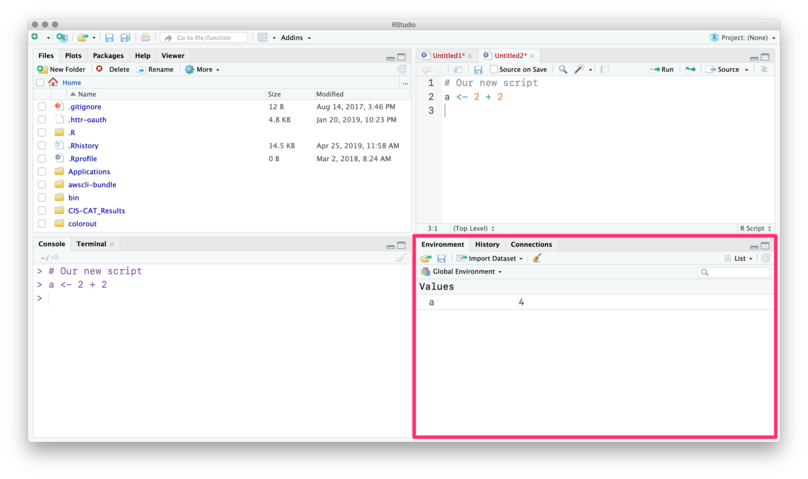
\includegraphics{img/rstudio_source_ex3.png}
\caption{Environment pane}
\end{figure}

\begin{center}\rule{0.5\linewidth}{\linethickness}\end{center}

The \emph{History} tab records your old commands.

\begin{figure}
\centering
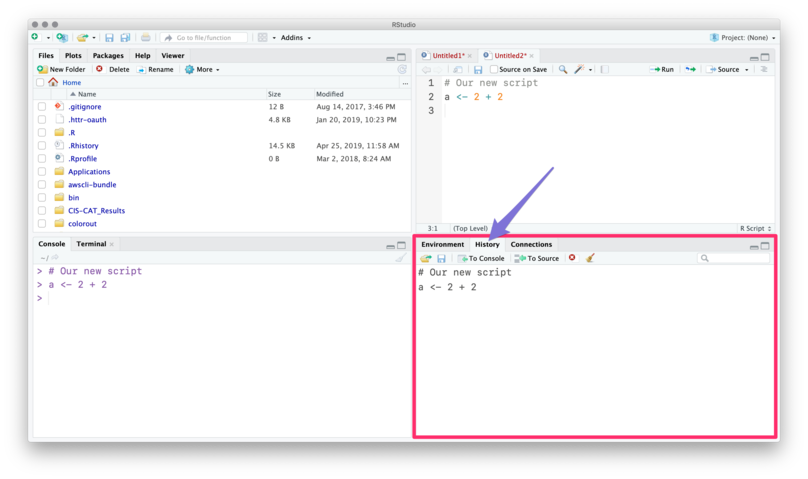
\includegraphics{img/rstudio_history.png}
\caption{History pane}
\end{figure}

\begin{center}\rule{0.5\linewidth}{\linethickness}\end{center}

The \emph{Files} pane is the file explorer.

\begin{figure}
\centering
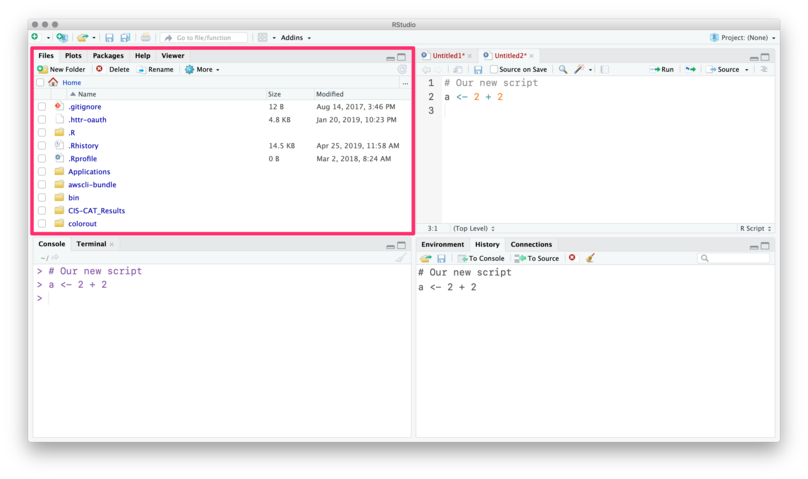
\includegraphics{img/rstudio_files.png}
\caption{Files pane}
\end{figure}

\begin{center}\rule{0.5\linewidth}{\linethickness}\end{center}

The \emph{Plots} pane/tab shows\ldots{} plots.

\begin{figure}
\centering
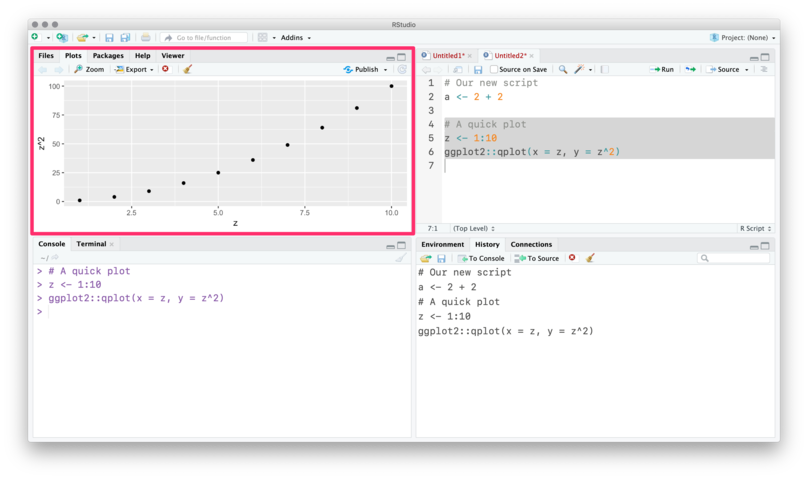
\includegraphics{img/rstudio_plots.png}
\caption{Plots pane}
\end{figure}

\begin{center}\rule{0.5\linewidth}{\linethickness}\end{center}

\emph{Packages} shows installed packages

\begin{figure}
\centering
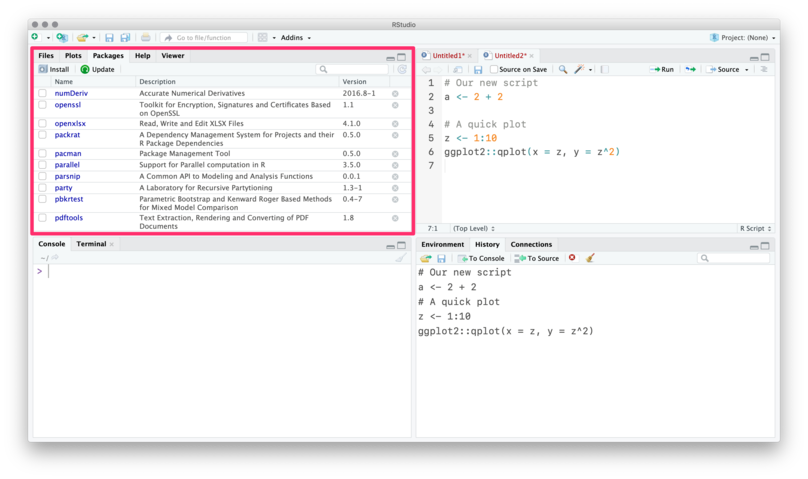
\includegraphics{img/rstudio_packages.png}
\caption{Packages pane}
\end{figure}

\begin{center}\rule{0.5\linewidth}{\linethickness}\end{center}

\emph{Packages} shows installed packages and whether they are \emph{loaded}.

\begin{figure}
\centering
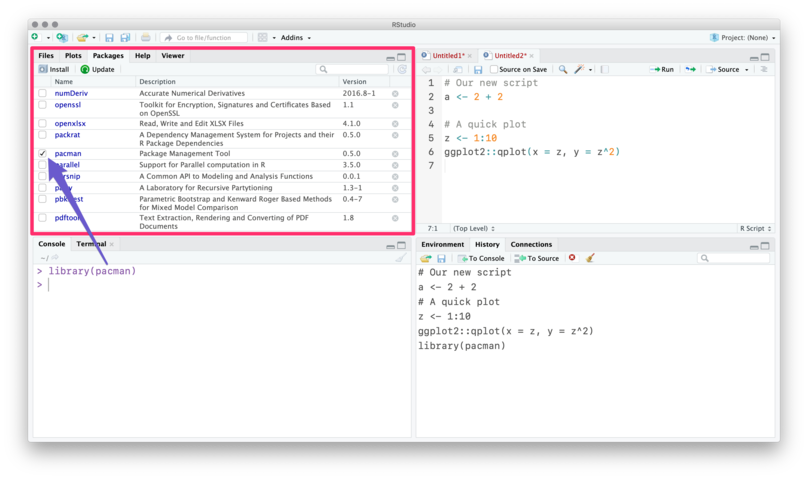
\includegraphics{img/rstudio_packages2.png}
\caption{Loaded and installed packages}
\end{figure}

\begin{center}\rule{0.5\linewidth}{\linethickness}\end{center}

The \emph{Help} tab shows help documentation (also accessible via \texttt{?}).

\begin{figure}
\centering
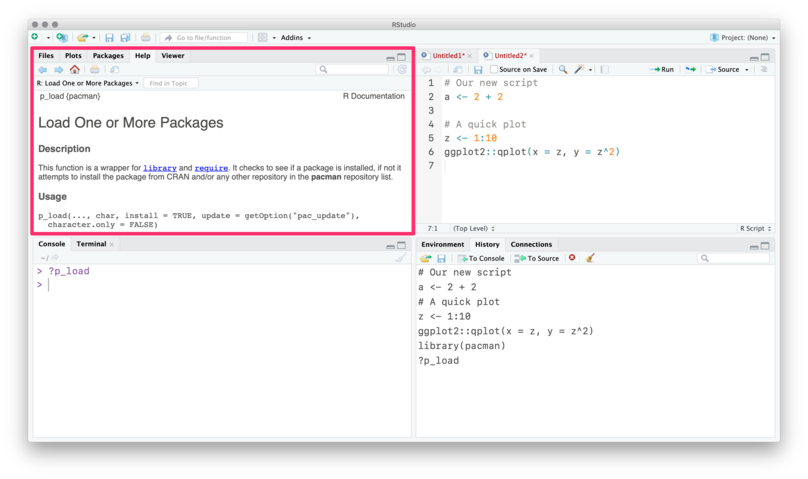
\includegraphics{img/rstudio_help.png}
\caption{Help pane}
\end{figure}

\begin{center}\rule{0.5\linewidth}{\linethickness}\end{center}

Finally, you can customize the actual layout

\begin{figure}
\centering
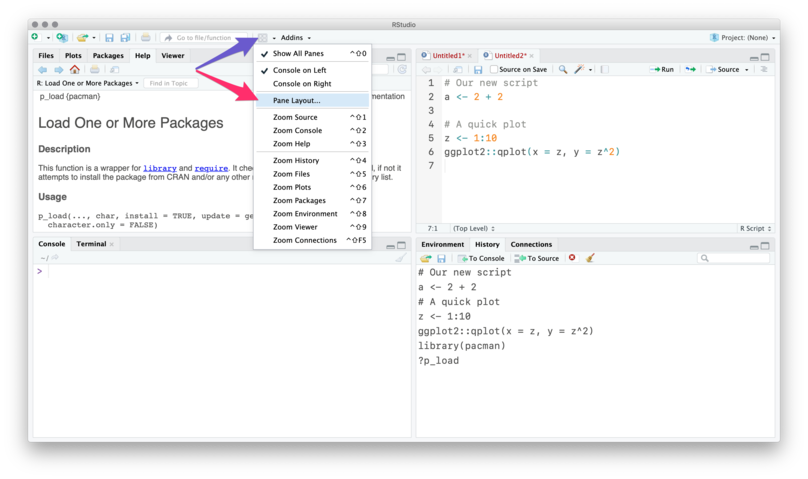
\includegraphics{img/rstudio_layout.png}
\caption{Customize layout}
\end{figure}

\hypertarget{rstudio-addins}{%
\section{RStudio addins}\label{rstudio-addins}}

RStudio can be further enhanced by so called ``addins''.
These are clickable snippets that execute certain actions in RStudio.

They aim to make repetitive tasks easier and to save you time.
There is an addin called \href{https://github.com/daattali/addinslist}{addinslist} which lists all available addins.
It can be installed as a normal package from CRAN:

\texttt{install.packages("addinslist")}

To have an addin available in RStudio after installation, RStudio needs to be restarted.

\hypertarget{rstudio-projects}{%
\section{RStudio projects}\label{rstudio-projects}}

Without a project, you will need to define \textbf{long} file paths which \textbf{only exist on your machine}.

\begin{Shaded}
\begin{Highlighting}[]
\NormalTok{sample_df <-}\StringTok{ }\KeywordTok{read.csv}\NormalTok{(}\StringTok{"/Users/<yourname>/somewhere/on/this/machine/sample.csv"}\NormalTok{)}
\end{Highlighting}
\end{Shaded}

With a project, R automatically references the project's folder as the current working directory.

From there on, you can use \emph{relative paths} to point to files.

\begin{Shaded}
\begin{Highlighting}[]
\NormalTok{sample_df <-}\StringTok{ }\KeywordTok{read.csv}\NormalTok{(}\StringTok{"sample.csv"}\NormalTok{)}
\end{Highlighting}
\end{Shaded}

\textbf{Double-plus bonus}: The \href{https://github.com/r-lib/here}{\emph{here}} package extends \emph{RStudio project} philosophy even more and helps in cases when not using RStudio (e.g.~on the command line).

\begin{figure}

\hfill{}
\includegraphics[width=11.11in]{img/here} 

\caption{© Allison Horst}\label{fig:unnamed-chunk-5}
\end{figure}

\hypertarget{alternatives-to-rstudio}{%
\section{Alternatives to RStudio}\label{alternatives-to-rstudio}}

\begin{itemize}
\item
  Using R directly in the terminal via \href{https://github.com/randy3k/radian}{radian} (optimized R console interpreter)
\item
  R is supported in other ``general purpose IDE's'' (VScode, Sublime Text, Atom, Vim, etc.)
\end{itemize}

\hypertarget{vis-basics}{%
\chapter{Visualization}\label{vis-basics}}

\begin{quote}
Embracing the grammar of graphics.
\end{quote}

This chapter discusses plotting with the \href{https://ggplot2.tidyverse.org/}{ggplot2 package}.

\begin{figure}

\hfill{}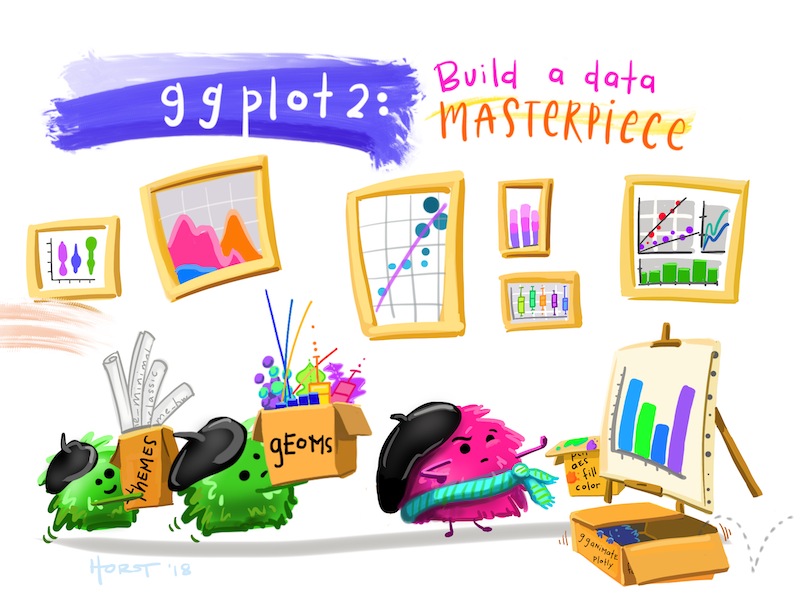
\includegraphics[width=11.11in]{img/ggplot2_masterpiece} 

\caption{© Allison Horst}\label{fig:unnamed-chunk-6}
\end{figure}

\hypertarget{basics-for-visualisation-in-r-using-ggplot2}{%
\section{Basics for visualisation in R using \{ggplot2\}}\label{basics-for-visualisation-in-r-using-ggplot2}}

\emph{Click here to show setup code.}

\begin{Shaded}
\begin{Highlighting}[]
\KeywordTok{library}\NormalTok{(tidyverse)}
\end{Highlighting}
\end{Shaded}

In the \{tidyverse\} the standard package for visualization is \{ggplot2\}.
The functions of this package follow a quite unique logic (the ``grammar of graphics'') and therefore require a special syntax.
In this section we want to give a short introduction, how to get started with \{ggplot2\}.

\begin{figure}

\hfill{}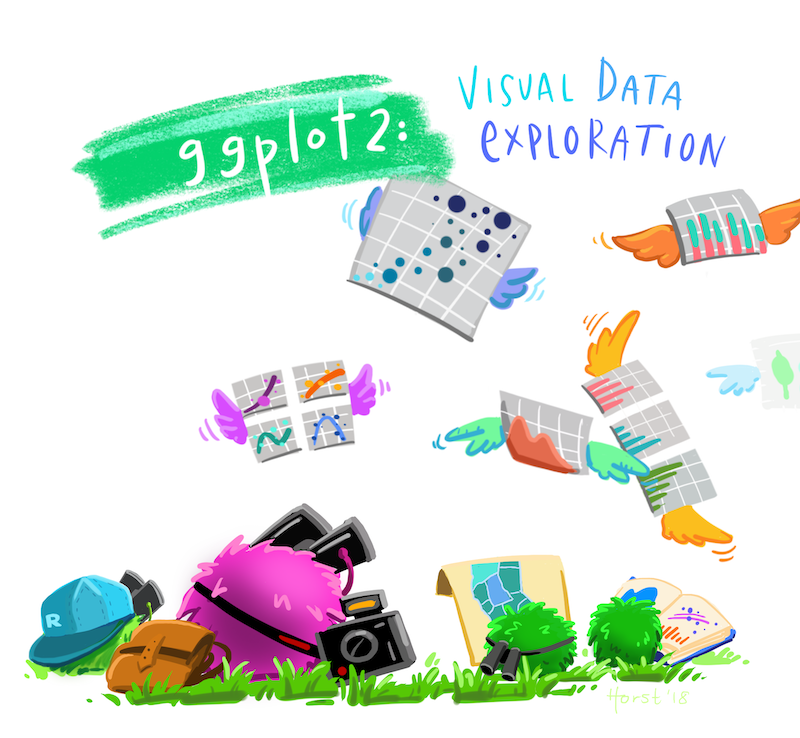
\includegraphics[width=11.11in]{img/ggplot2_exploratory} 

\caption{© Allison Horst}\label{fig:unnamed-chunk-29}
\end{figure}

\hypertarget{creating-the-plot-skeleton-ggplot}{%
\subsection{\texorpdfstring{Creating the plot skeleton: \texttt{ggplot()}}{Creating the plot skeleton: ggplot()}}\label{creating-the-plot-skeleton-ggplot}}

The main function in the package is \texttt{ggplot()}, which prepares/creates a graph.
By setting the arguments of the function, you can:

\begin{enumerate}
\def\labelenumi{\arabic{enumi}.}
\tightlist
\item
  Choose the dataset to be plotted (argument \texttt{data})
\item
  Choose the mapping of the variables to the axes (or further forms of setting apart data) in the argument \texttt{mapping}.
  This argument takes the result of the function \texttt{aes()}, which you will get to know in many different examples.
\end{enumerate}

\begin{Shaded}
\begin{Highlighting}[]
\KeywordTok{ggplot}\NormalTok{(}
  \DataTypeTok{data =}\NormalTok{ mpg,}
  \DataTypeTok{mapping =} \KeywordTok{aes}\NormalTok{(}\DataTypeTok{x =}\NormalTok{ displ, }\DataTypeTok{y =}\NormalTok{ hwy)}
\NormalTok{)}
\end{Highlighting}
\end{Shaded}

\begin{flushright}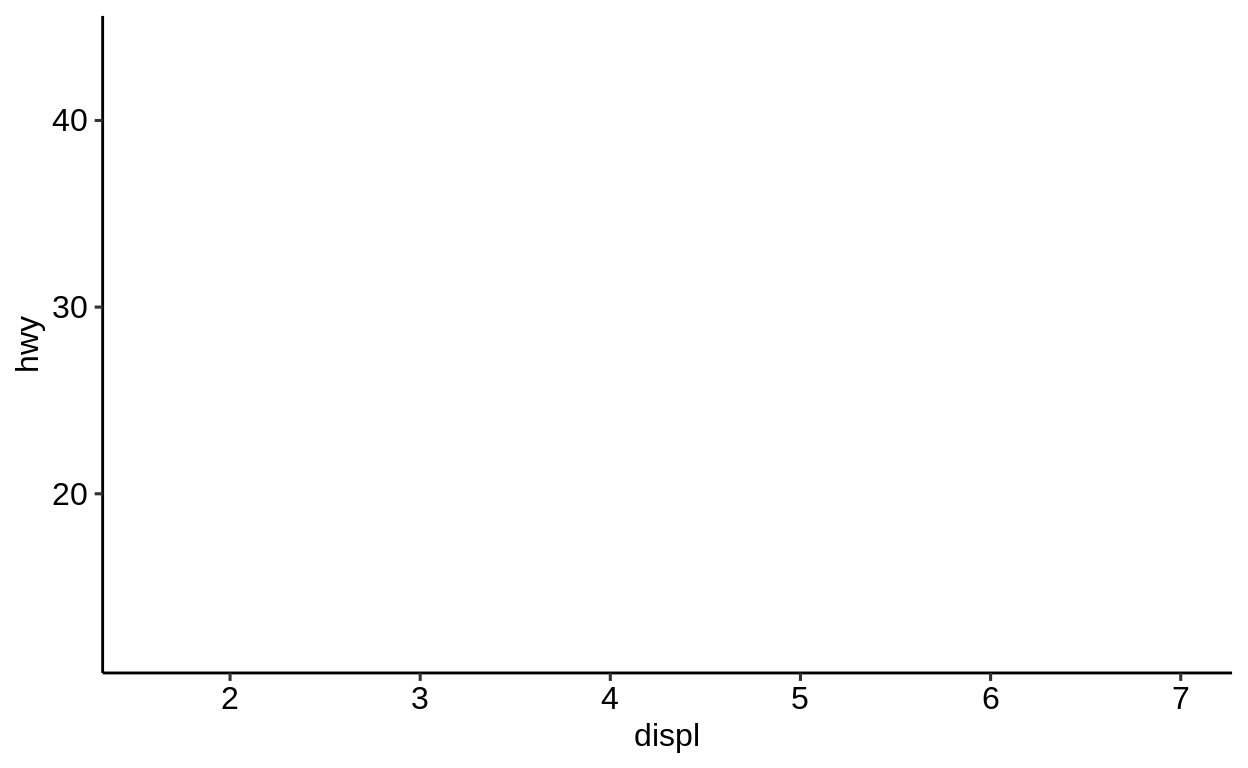
\includegraphics{vistransrep_files/figure-latex/101-empty-graph-1} \end{flushright}

This created only an empty plot, because we did not tell \{ggplot2\} which geometry we want to use to display the variables we set in the \texttt{ggplot()} call.
We do this by adding (with the help of the \texttt{+} operator after the \texttt{ggplot()}-call) a different function starting with \texttt{geom\_} to provide this information.

\begin{Shaded}
\begin{Highlighting}[]
\KeywordTok{ggplot}\NormalTok{(}
  \DataTypeTok{data =}\NormalTok{ mpg,}
  \DataTypeTok{mapping =} \KeywordTok{aes}\NormalTok{(}\DataTypeTok{x =}\NormalTok{ displ, }\DataTypeTok{y =}\NormalTok{ hwy)}
\NormalTok{) }\OperatorTok{+}
\StringTok{  }\KeywordTok{geom_point}\NormalTok{()}
\end{Highlighting}
\end{Shaded}

\begin{flushright}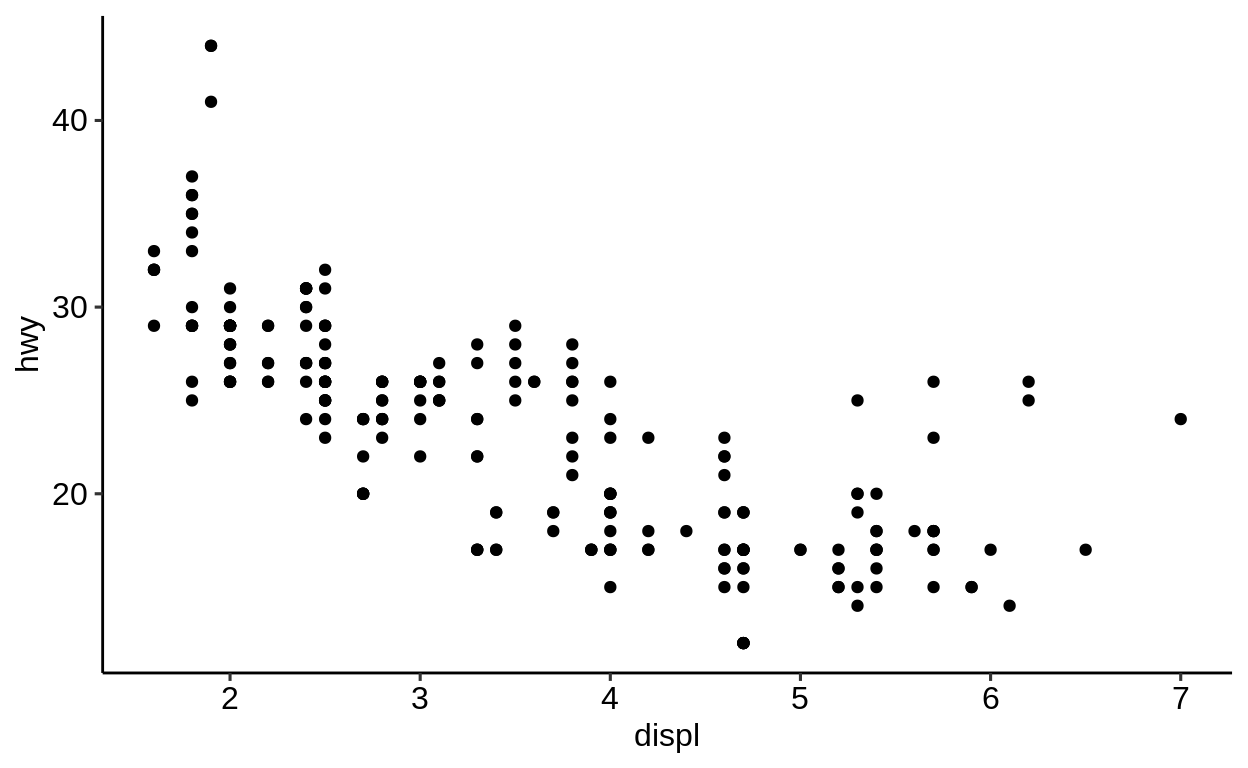
\includegraphics{vistransrep_files/figure-latex/101-visualize-variables-as-points-scatterplot-1} \end{flushright}

This is maybe the most basic plot you can create.
To map a different variable than \texttt{disp} to the x-axis, change the respective variable name in the \texttt{aes()} argument.

\begin{Shaded}
\begin{Highlighting}[]
\KeywordTok{ggplot}\NormalTok{(}
  \DataTypeTok{data =}\NormalTok{ mpg,}
  \DataTypeTok{mapping =} \KeywordTok{aes}\NormalTok{(}\DataTypeTok{x =}\NormalTok{ cyl, }\DataTypeTok{y =}\NormalTok{ hwy)}
\NormalTok{) }\OperatorTok{+}
\StringTok{  }\KeywordTok{geom_point}\NormalTok{()}
\end{Highlighting}
\end{Shaded}

\begin{flushright}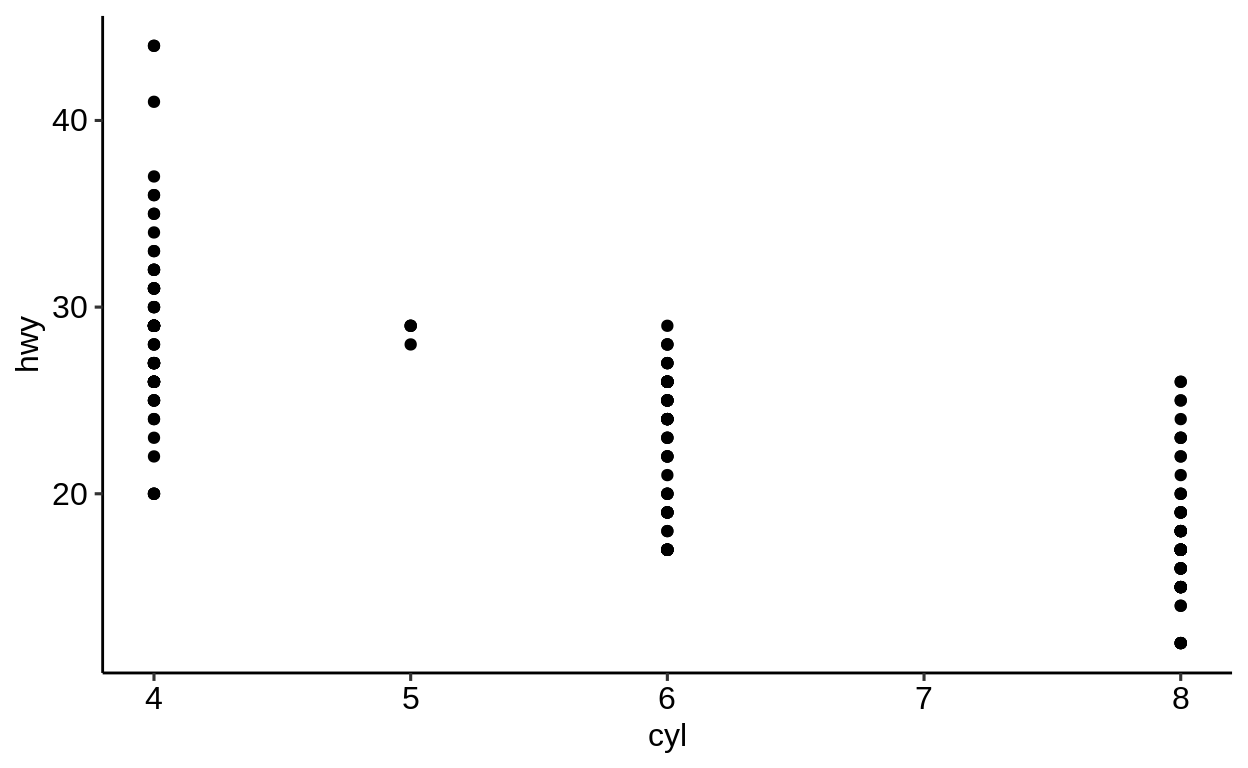
\includegraphics{vistransrep_files/figure-latex/101-aes-determines-which-variables-are-plotted-1} \end{flushright}

You can exchange the variables to be plotted freely, without changing anything else to the rest of the code.

\begin{Shaded}
\begin{Highlighting}[]
\KeywordTok{ggplot}\NormalTok{(}
  \DataTypeTok{data =}\NormalTok{ mpg,}
  \DataTypeTok{mapping =} \KeywordTok{aes}\NormalTok{(}\DataTypeTok{x =}\NormalTok{ hwy, }\DataTypeTok{y =}\NormalTok{ cty)}
\NormalTok{) }\OperatorTok{+}
\StringTok{  }\KeywordTok{geom_point}\NormalTok{()}
\end{Highlighting}
\end{Shaded}

\begin{flushright}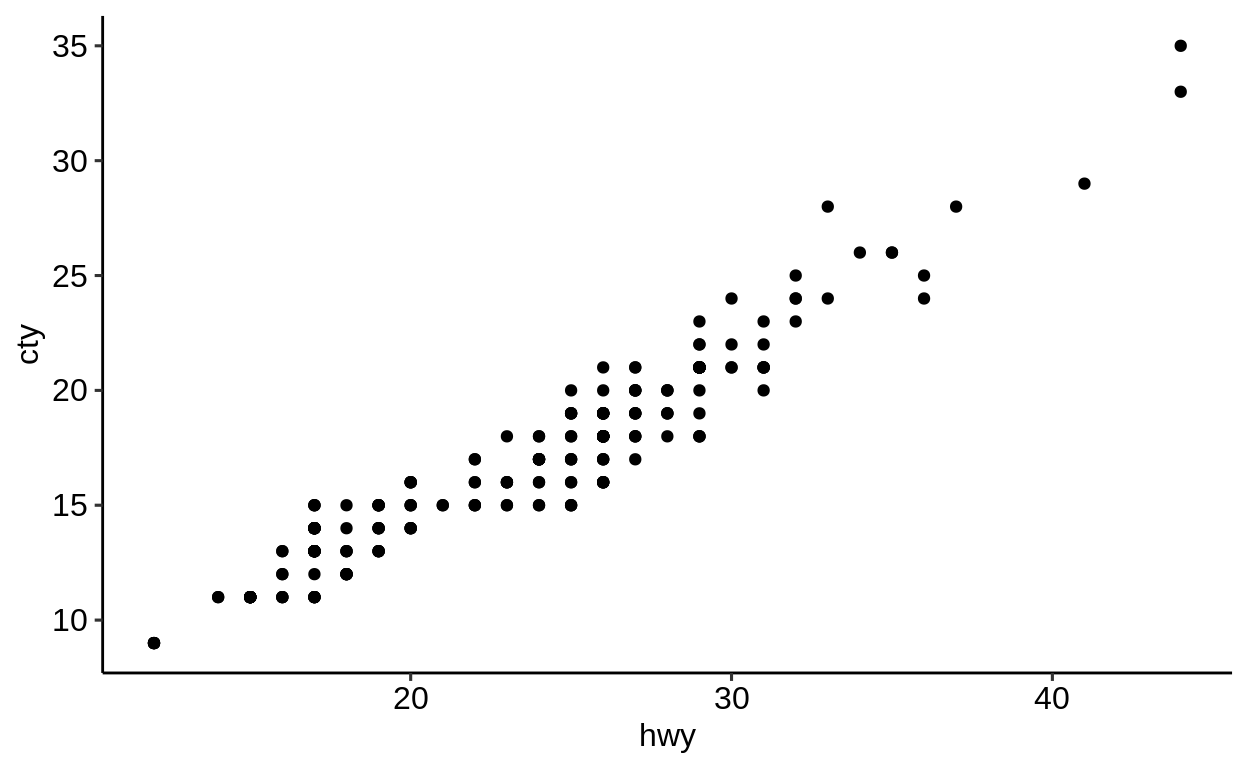
\includegraphics{vistransrep_files/figure-latex/101-pattern-unchanged-if-only-variables-are-plotted-1} \end{flushright}

Always good to have: The \emph{ggplot2} cheatsheet (\url{https://github.com/rstudio/cheatsheets/blob/master/data-visualization-2.1.pdf}).

\hypertarget{what-is-a-statistical-graphic}{%
\subsection{What is a ``statistical graphic''?}\label{what-is-a-statistical-graphic}}

Wilkinson (2005) defines a grammar to describe the basic elements of a
statistical graphic:

\begin{quote}
``{[}\ldots{}{]} a statistical graphic is a mapping from data to
aesthetic attributes (colour, shape, size) of geometric objects
(points, line, bars).''
\end{quote}

\hfill (Wickham, 2009)

\hypertarget{terminology}{%
\subsection{Terminology}\label{terminology}}

\begin{itemize}
\item
  \textbf{Data:} The data to visualize -- consists of variables and observations.
\item
  \textbf{Geoms:} Geometric objects which represent the data (points, lines, polygons, etc.).
\item
  \textbf{Mappings:} Match variables with aesthetic attributes of the (geometric) objects.
\item
  \textbf{Scales:} Mapping of the ``data units'' to ``physical units'' of the geometric objects (e.g.~length, diameter or color); defines the \emph{legend}.
\item
  \textbf{Coord:} System of coordinates, mapping of the data to a two dimensional plain of the graphic; defines the \emph{axes} and \emph{grid}.
\item
  \textbf{Stats:} Statistical transformation of the data (5 point summary, classification, etc.).
\item
  \textbf{Facetting:} Division and illustration of data subsets, also known as ``Trellis'' images.
\end{itemize}

\hypertarget{the-grammar-of-graphics}{%
\subsection{The Grammar of graphics \ldots{}}\label{the-grammar-of-graphics}}

\textbf{is \ldots{}}

a formal guideline which describes the dependencies between all elements of a
statistical graphic.

\textbf{isn't \ldots{}}

\begin{itemize}
\tightlist
\item
  a manual which tells us \emph{which graphic} should be created for a given question.
\item
  a specification \emph{how} a statistical graphic should look like.
\end{itemize}

\hypertarget{about-ggplot2}{%
\subsection{About \{ggplot2\}}\label{about-ggplot2}}

\begin{verbatim}
## Package: ggplot2
## Version: 3.2.1
## Title: Create Elegant Data Visualisations Using the Grammar of Graphics
## Depends: R (>= 3.2)
## Imports: digest, grDevices, grid, gtable (>= 0.1.1), lazyeval, MASS, mgcv,
##          reshape2, rlang (>= 0.3.0), scales (>= 0.5.0), stats, tibble,
##          viridisLite, withr (>= 2.0.0)
## License: GPL-2 | file LICENSE
## URL: http://ggplot2.tidyverse.org, https://github.com/tidyverse/ggplot2
## BugReports: https://github.com/tidyverse/ggplot2/issues
## Encoding: UTF-8
## Author: Hadley Wickham [aut, cre], Winston Chang [aut], Lionel Henry [aut],
##          Thomas Lin Pedersen [aut], Kohske Takahashi [aut], Claus Wilke [aut],
##          Kara Woo [aut], Hiroaki Yutani [aut], RStudio [cph]
## Maintainer: Hadley Wickham <hadley@rstudio.com>
## 
## -- File:
\end{verbatim}

\hypertarget{geom_-functions}{%
\section{\texorpdfstring{\texttt{geom\_*} functions}{geom\_* functions}}\label{geom_-functions}}

\emph{Click here to show setup code.}

\begin{Shaded}
\begin{Highlighting}[]
\KeywordTok{library}\NormalTok{(tidyverse)}
\end{Highlighting}
\end{Shaded}

\texttt{geom\_*} functions are added to the main \texttt{ggplot()} call via the ``+'' operator and
(usually) placed on a new line.

A list of all available ``geoms'' can be found here:

\url{https://ggplot2.tidyverse.org/reference/\#section-layer-geoms}

The most popular ones are

\begin{itemize}
\item
  \texttt{geom\_point()}
\item
  \texttt{geom\_histogram()}
\item
  \texttt{geom\_boxplot()}
\item
  \texttt{geom\_bar()}
\end{itemize}

\begin{center}\rule{0.5\linewidth}{\linethickness}\end{center}

The \texttt{geom\_*} family can be divided into three parts:

\textbf{One variable plots}

\begin{itemize}
\tightlist
\item
  \texttt{geom\_hist()}
\item
  \texttt{geom\_bar()}
\item
  etc.
\end{itemize}

\textbf{Two variable plots}

\begin{itemize}
\tightlist
\item
  \texttt{geom\_point()}
\item
  \texttt{geom\_line()}
\item
  \texttt{geom\_boxplot()}
\item
  etc.
\end{itemize}

\textbf{Three variables plots}

\begin{itemize}
\tightlist
\item
  \texttt{geom\_raster()}
\item
  \texttt{geom\_sf()}
\item
  \texttt{geom\_tile()}
\item
  etc.
\end{itemize}

\hypertarget{arguments}{%
\subsection{Arguments}\label{arguments}}

\begin{Shaded}
\begin{Highlighting}[]
\KeywordTok{ggplot}\NormalTok{(data, }\DataTypeTok{mapping =} \KeywordTok{aes}\NormalTok{(), ...) }\OperatorTok{+}
\StringTok{  }\KeywordTok{geom_XXX}\NormalTok{(}\DataTypeTok{mapping =} \OtherTok{NULL}\NormalTok{, }\DataTypeTok{data =} \OtherTok{NULL}\NormalTok{, stat, ...)}
\end{Highlighting}
\end{Shaded}

\texttt{geom\_*} functions have the same basic arguments as \texttt{ggplot()}.
In addition, they come with more arguments specific to the respective ``geom''.

\textbf{stat}

The \texttt{stat} parameter defines a statistical transformation:

\begin{itemize}
\item
  if set to \texttt{"identity"}: No transformation
\item
  if set to \texttt{boxplot}: Boxplot transformation
\item
  etc.
\end{itemize}

\textbf{position}

The same applies to the \texttt{position} argument.
In the example below, points are not adjusted and just visualized where they appear in the data.

In the case of boxplots, a special position arrangement function is used to arrange everything nicely: \texttt{position\_dodge2()} (here denoted by \texttt{position\ =\ "dodge2"}).

\begin{Shaded}
\begin{Highlighting}[]
\KeywordTok{geom_point}\NormalTok{(}\DataTypeTok{mapping =} \OtherTok{NULL}\NormalTok{, }\DataTypeTok{data =} \OtherTok{NULL}\NormalTok{, }\DataTypeTok{stat =} \StringTok{"identity"}\NormalTok{,}
  \DataTypeTok{position =} \StringTok{"identity"}\NormalTok{, ..., }\DataTypeTok{na.rm =} \OtherTok{FALSE}\NormalTok{, }\DataTypeTok{show.legend =} \OtherTok{NA}\NormalTok{,}
  \DataTypeTok{inherit.aes =} \OtherTok{TRUE}\NormalTok{)}

\KeywordTok{geom_boxplot}\NormalTok{(}\DataTypeTok{mapping =} \OtherTok{NULL}\NormalTok{, }\DataTypeTok{data =} \OtherTok{NULL}\NormalTok{, }\DataTypeTok{stat =} \StringTok{"boxplot"}\NormalTok{,}
  \DataTypeTok{position =} \StringTok{"dodge2"}\NormalTok{, ..., }\DataTypeTok{outlier.colour =} \OtherTok{NULL}\NormalTok{,}
  \DataTypeTok{outlier.color =} \OtherTok{NULL}\NormalTok{, }\DataTypeTok{outlier.fill =} \OtherTok{NULL}\NormalTok{, }\DataTypeTok{outlier.shape =} \DecValTok{19}\NormalTok{,}
  \DataTypeTok{outlier.size =} \FloatTok{1.5}\NormalTok{, }\DataTypeTok{outlier.stroke =} \FloatTok{0.5}\NormalTok{, }\DataTypeTok{outlier.alpha =} \OtherTok{NULL}\NormalTok{,}
  \DataTypeTok{notch =} \OtherTok{FALSE}\NormalTok{, }\DataTypeTok{notchwidth =} \FloatTok{0.5}\NormalTok{, }\DataTypeTok{varwidth =} \OtherTok{FALSE}\NormalTok{, }\DataTypeTok{na.rm =} \OtherTok{FALSE}\NormalTok{,}
  \DataTypeTok{show.legend =} \OtherTok{NA}\NormalTok{, }\DataTypeTok{inherit.aes =} \OtherTok{TRUE}\NormalTok{)}
\end{Highlighting}
\end{Shaded}

\begin{center}\rule{0.5\linewidth}{\linethickness}\end{center}

\texttt{geom\_boxplot()} needs one variable to be of class \texttt{character} or \texttt{factor} (better) to initiate the grouping.

\begin{Shaded}
\begin{Highlighting}[]
\KeywordTok{class}\NormalTok{(mpg}\OperatorTok{$}\NormalTok{class)}
\end{Highlighting}
\end{Shaded}

\begin{verbatim}
## [1] "character"
\end{verbatim}

\begin{Shaded}
\begin{Highlighting}[]
\KeywordTok{ggplot}\NormalTok{(mpg, }\KeywordTok{aes}\NormalTok{(}\DataTypeTok{x =}\NormalTok{ class, }\DataTypeTok{y =}\NormalTok{ displ)) }\OperatorTok{+}
\StringTok{  }\KeywordTok{geom_boxplot}\NormalTok{()}
\end{Highlighting}
\end{Shaded}

\begin{flushright}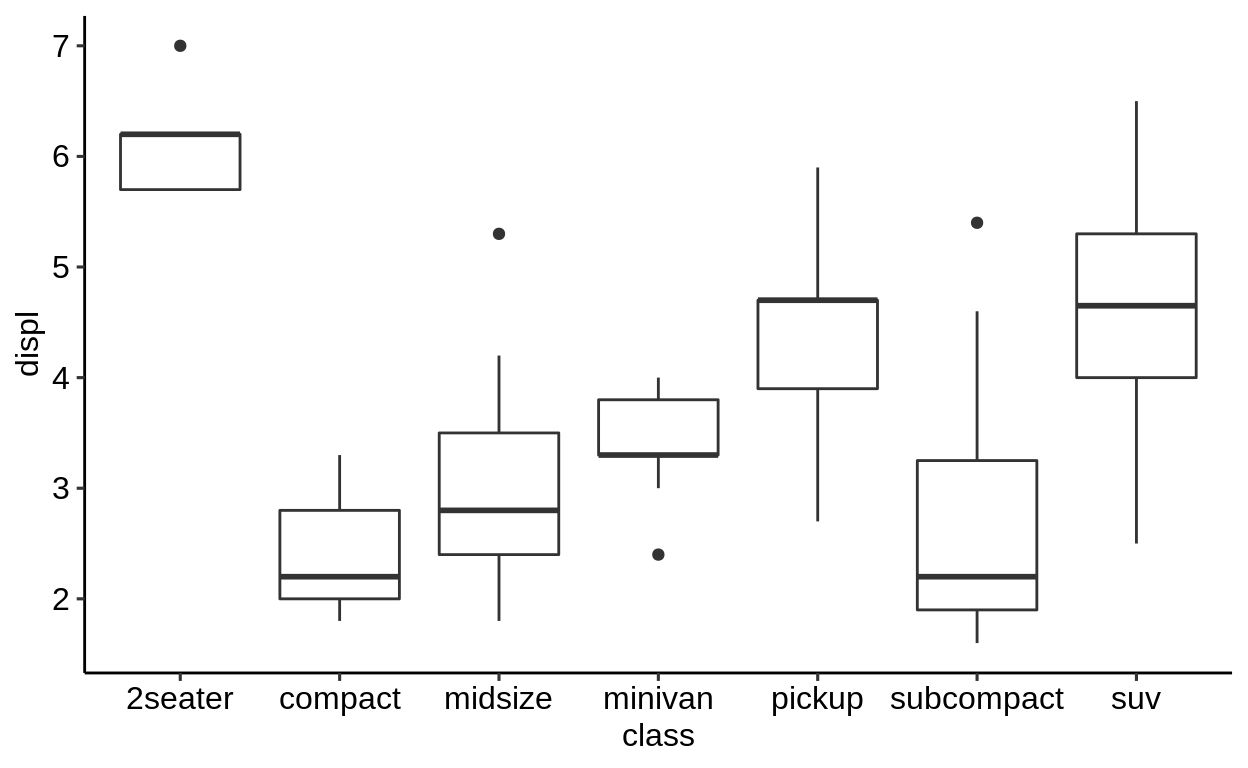
\includegraphics{vistransrep_files/figure-latex/12-show-geom-boxplot-1} \end{flushright}

\hypertarget{combining-geoms}{%
\subsection{Combining geoms}\label{combining-geoms}}

Multiple \texttt{geom\_*} functions can be used in one plot.
A combination that is often used together is \texttt{geom\_point()} and \texttt{geom\_smooth()}

\begin{Shaded}
\begin{Highlighting}[]
\KeywordTok{ggplot}\NormalTok{(mpg, }\KeywordTok{aes}\NormalTok{(}\DataTypeTok{x =}\NormalTok{ displ, }\DataTypeTok{y =}\NormalTok{ hwy)) }\OperatorTok{+}
\StringTok{  }\KeywordTok{geom_point}\NormalTok{() }\OperatorTok{+}
\StringTok{  }\KeywordTok{geom_smooth}\NormalTok{(}\DataTypeTok{method =} \StringTok{"lm"}\NormalTok{)}
\end{Highlighting}
\end{Shaded}

\begin{flushright}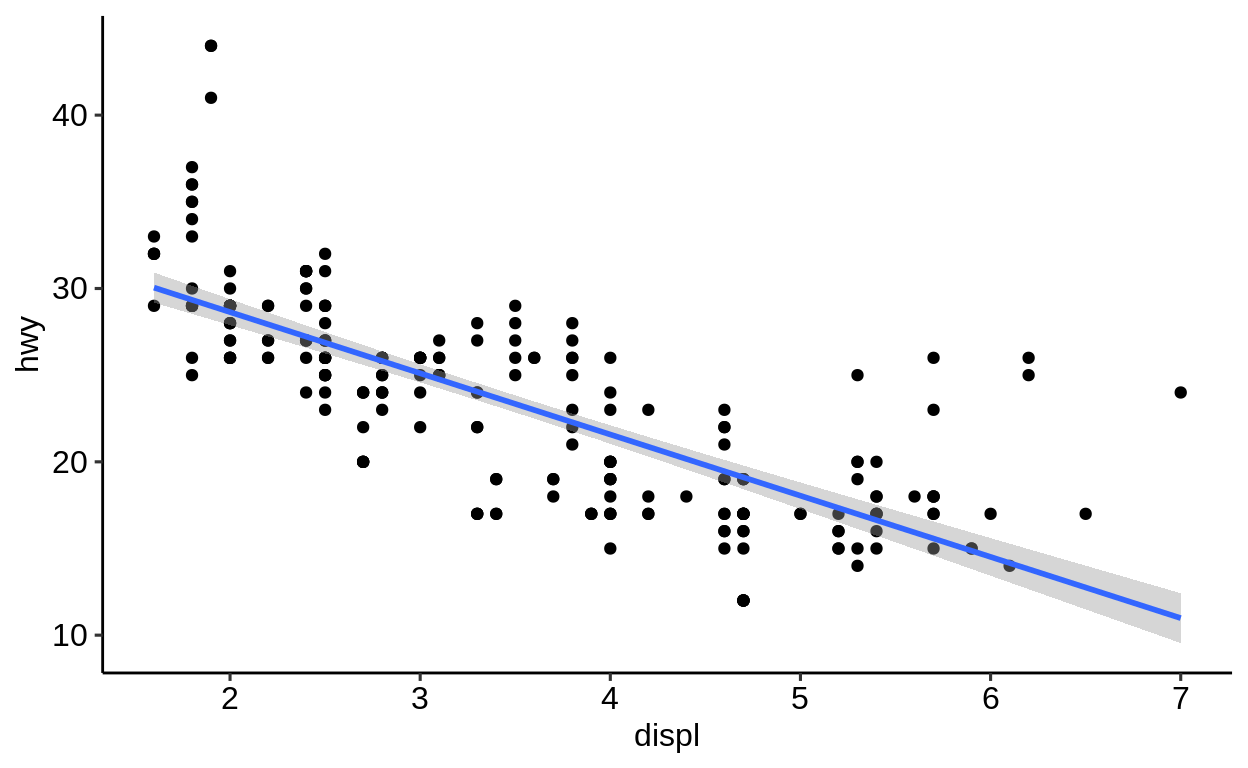
\includegraphics{vistransrep_files/figure-latex/12-combining-multiple-geoms-1} \end{flushright}

Unless specified differently in the \texttt{geom\_*()} call, all geoms will use the same variables.

\hypertarget{summary}{%
\subsection{Summary}\label{summary}}

The modular principle of \texttt{ggplot2} enables:

\begin{itemize}
\tightlist
\item
  the combination of any geometric objects (geoms).
\item
  a high flexibility and customizability
\end{itemize}

An extensive description of all geometric objects can be found on the \texttt{ggplot2} website \url{https://ggplot2.tidyverse.org/reference/}.

\textbf{Exercises}

\url{https://krlmlr.github.io/vistransrep/2019-11-zhr/geoms.html}

\hypertarget{two-variable-plots}{%
\section{Two variable plots}\label{two-variable-plots}}

\emph{Click here to show setup code.}

\begin{Shaded}
\begin{Highlighting}[]
\KeywordTok{library}\NormalTok{(tidyverse)}
\end{Highlighting}
\end{Shaded}

``Two variable plots'' can be split into sub-categories:

\begin{itemize}
\item
  Continuous X and Y
\item
  Continuous X and discrete Y (and vice-versa)
\item
  Discrete X and Y
\end{itemize}

\hypertarget{continuous-x-and-y}{%
\subsection{Continuous X and Y}\label{continuous-x-and-y}}

\begin{Shaded}
\begin{Highlighting}[]
\KeywordTok{ggplot}\NormalTok{(mpg, }\KeywordTok{aes}\NormalTok{(}\DataTypeTok{x =}\NormalTok{ cty, }\DataTypeTok{y =}\NormalTok{ hwy)) }\OperatorTok{+}
\StringTok{  }\KeywordTok{geom_point}\NormalTok{()}
\end{Highlighting}
\end{Shaded}

\begin{flushright}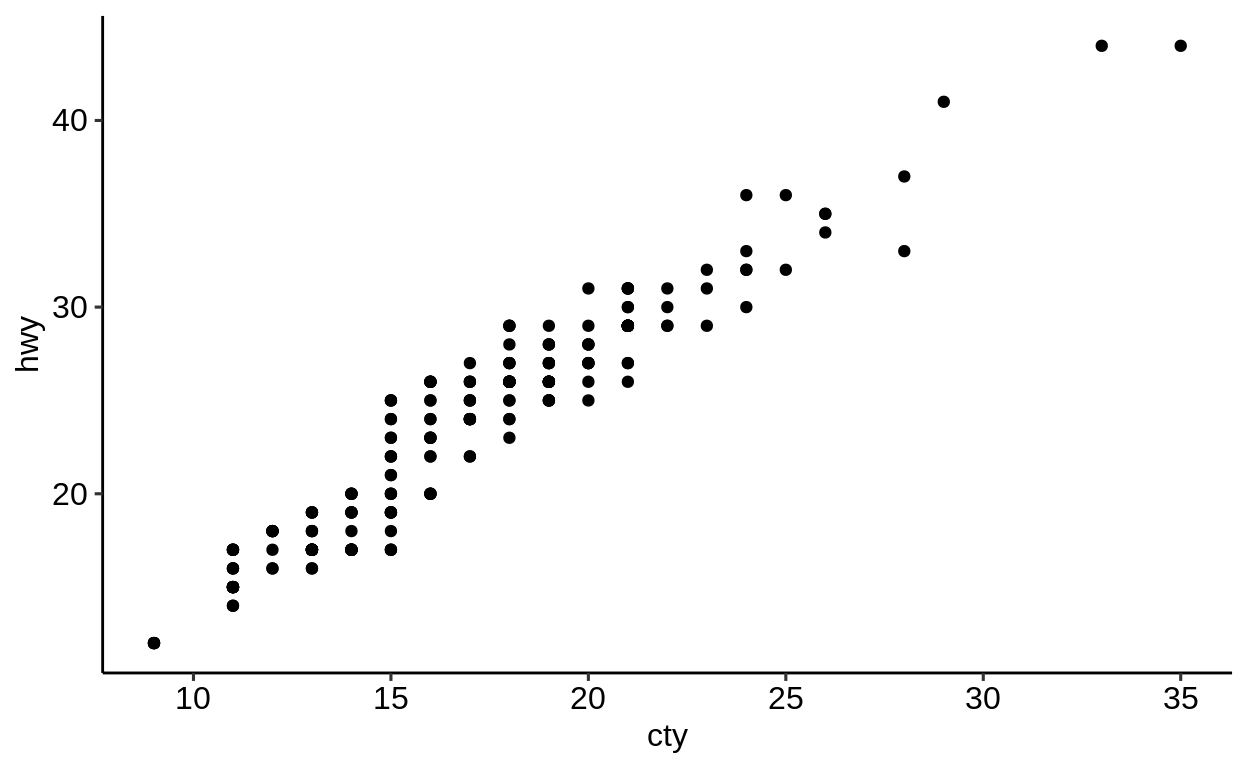
\includegraphics{vistransrep_files/figure-latex/13-continuous-x-and-y-1} \end{flushright}

\begin{center}\rule{0.5\linewidth}{\linethickness}\end{center}

\hypertarget{discrete-x-and-continuous-y}{%
\subsection{Discrete X and continuous Y}\label{discrete-x-and-continuous-y}}

\begin{Shaded}
\begin{Highlighting}[]
\KeywordTok{ggplot}\NormalTok{(mpg, }\KeywordTok{aes}\NormalTok{(}\DataTypeTok{x =}\NormalTok{ class, }\DataTypeTok{y =}\NormalTok{ hwy)) }\OperatorTok{+}
\StringTok{  }\KeywordTok{geom_boxplot}\NormalTok{()}
\end{Highlighting}
\end{Shaded}

\begin{flushright}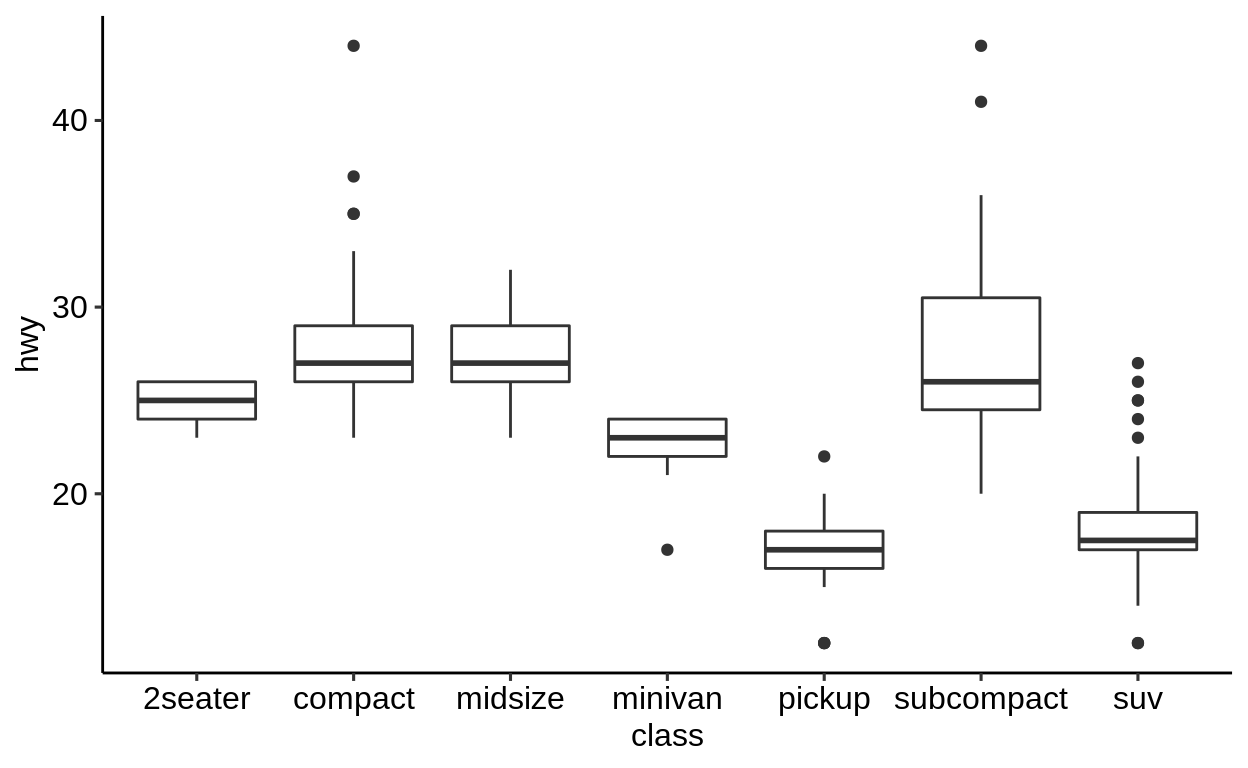
\includegraphics{vistransrep_files/figure-latex/13-discrete-x-and-continuous-y-1} \end{flushright}

\begin{center}\rule{0.5\linewidth}{\linethickness}\end{center}

\hypertarget{discrete-x-and-y}{%
\subsection{Discrete X and Y}\label{discrete-x-and-y}}

\begin{Shaded}
\begin{Highlighting}[]
\KeywordTok{ggplot}\NormalTok{(mpg, }\KeywordTok{aes}\NormalTok{(}\DataTypeTok{x =}\NormalTok{ class, }\DataTypeTok{y =}\NormalTok{ manufacturer)) }\OperatorTok{+}
\StringTok{  }\KeywordTok{geom_jitter}\NormalTok{()}
\end{Highlighting}
\end{Shaded}

\begin{flushright}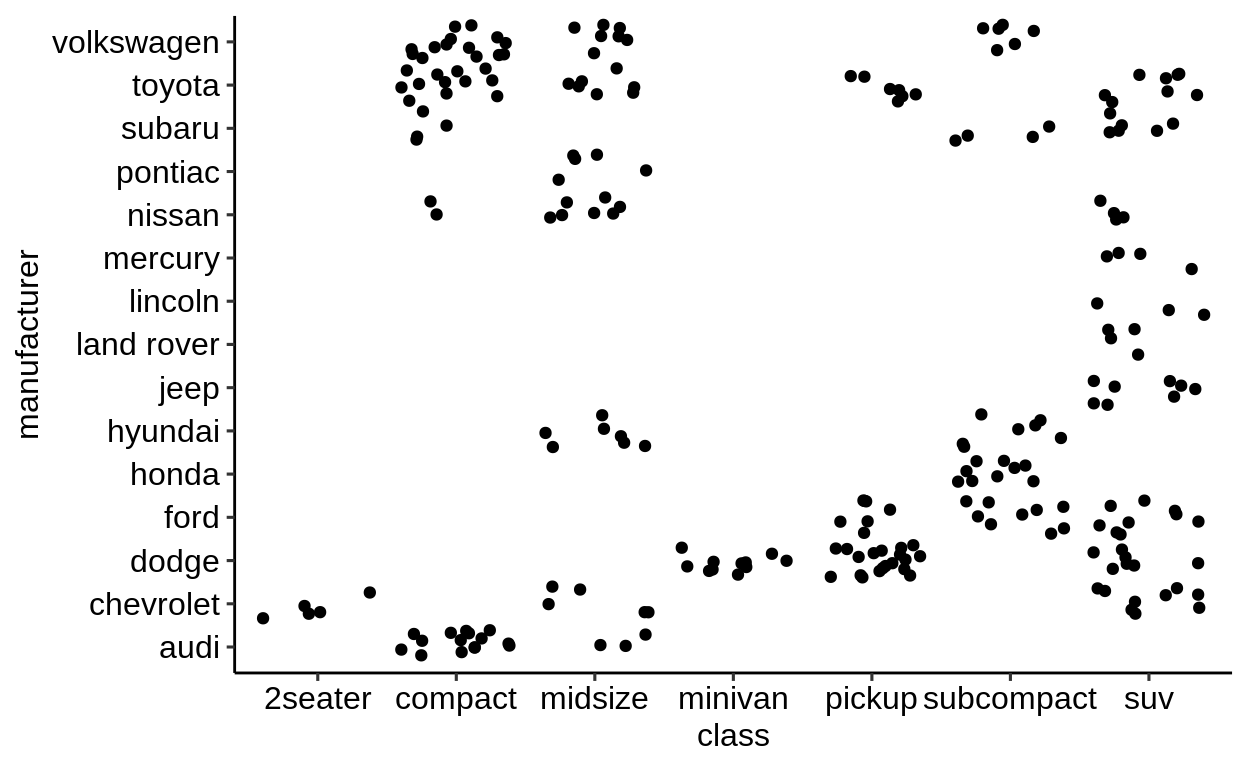
\includegraphics{vistransrep_files/figure-latex/13-discrete-x-and-y-1} \end{flushright}

\hypertarget{one-variable-plots}{%
\section{One variable plots}\label{one-variable-plots}}

\emph{Click here to show setup code.}

\begin{Shaded}
\begin{Highlighting}[]
\KeywordTok{library}\NormalTok{(tidyverse)}
\end{Highlighting}
\end{Shaded}

This type of plots visualizes ONE variable in a certain way.

To do this in a 2D space, a \textbf{statistical transformation} of the variable is required for the missing axis.

\hypertarget{continuous-variables}{%
\subsection{Continuous variables}\label{continuous-variables}}

\begin{itemize}
\item
  Histogram: Most common way - grouping the variable into equal bins
\item
  \texttt{geom\_density()}, \texttt{geom\_freq()}, \texttt{geom\_dotplot()} and \texttt{geom\_area()} are mainly doing the same as \texttt{geom\_hist()}
\end{itemize}

We supply only \emph{one} variable to the \texttt{mapping} argument with the help of \texttt{aes()}.
This one is automatically grouped into 30 bins.

\begin{Shaded}
\begin{Highlighting}[]
\KeywordTok{ggplot}\NormalTok{(mpg, }\KeywordTok{aes}\NormalTok{(}\DataTypeTok{x =}\NormalTok{ hwy)) }\OperatorTok{+}
\StringTok{  }\KeywordTok{geom_histogram}\NormalTok{()}
\end{Highlighting}
\end{Shaded}

\begin{verbatim}
## `stat_bin()` using `bins = 30`. Pick better value with
## `binwidth`.
\end{verbatim}

\begin{flushright}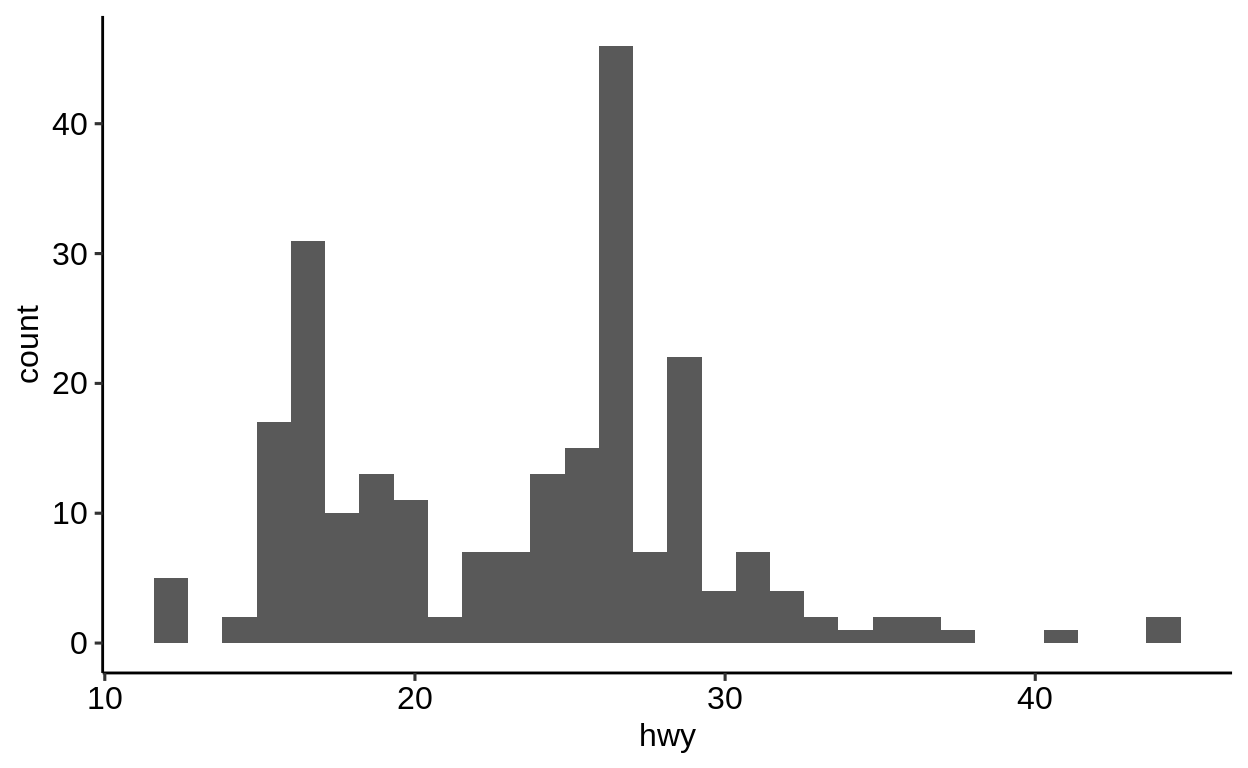
\includegraphics{vistransrep_files/figure-latex/14-continuous-variables-histogram-most-common-1} \end{flushright}

\begin{center}\rule{0.5\linewidth}{\linethickness}\end{center}

\begin{Shaded}
\begin{Highlighting}[]
\KeywordTok{ggplot}\NormalTok{(mpg, }\KeywordTok{aes}\NormalTok{(}\DataTypeTok{x =}\NormalTok{ hwy)) }\OperatorTok{+}
\StringTok{  }\KeywordTok{geom_density}\NormalTok{()}
\end{Highlighting}
\end{Shaded}

\begin{flushright}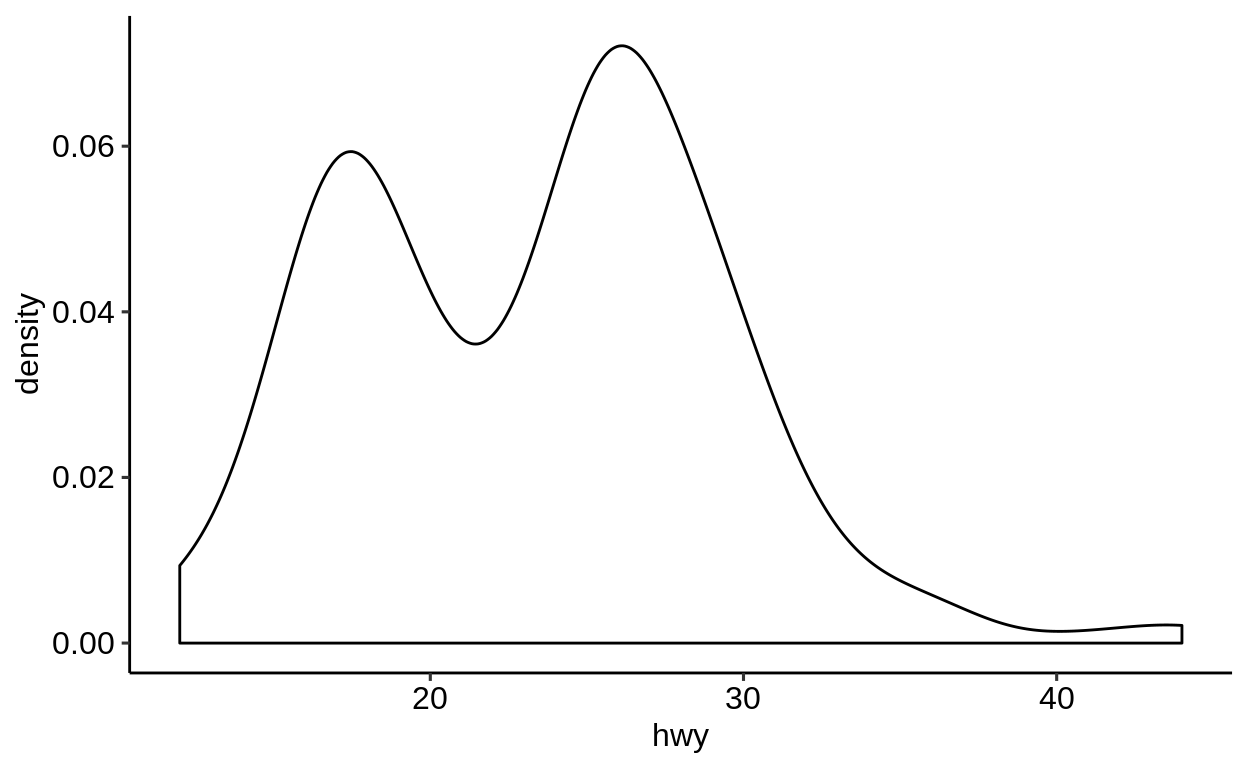
\includegraphics{vistransrep_files/figure-latex/14-showcase-density-1} \end{flushright}

\hypertarget{discrete-variables}{%
\subsection{Discrete variables}\label{discrete-variables}}

For discrete data, there is actually only one visualization method - the bar plot.

\smallskip

\emph{Note the difference of \texttt{geom\_bar()} compared to \texttt{geom\_hist()}.}

\begin{Shaded}
\begin{Highlighting}[]
\KeywordTok{ggplot}\NormalTok{(mpg, }\KeywordTok{aes}\NormalTok{(fl)) }\OperatorTok{+}
\StringTok{  }\KeywordTok{geom_bar}\NormalTok{()}
\end{Highlighting}
\end{Shaded}

\begin{flushright}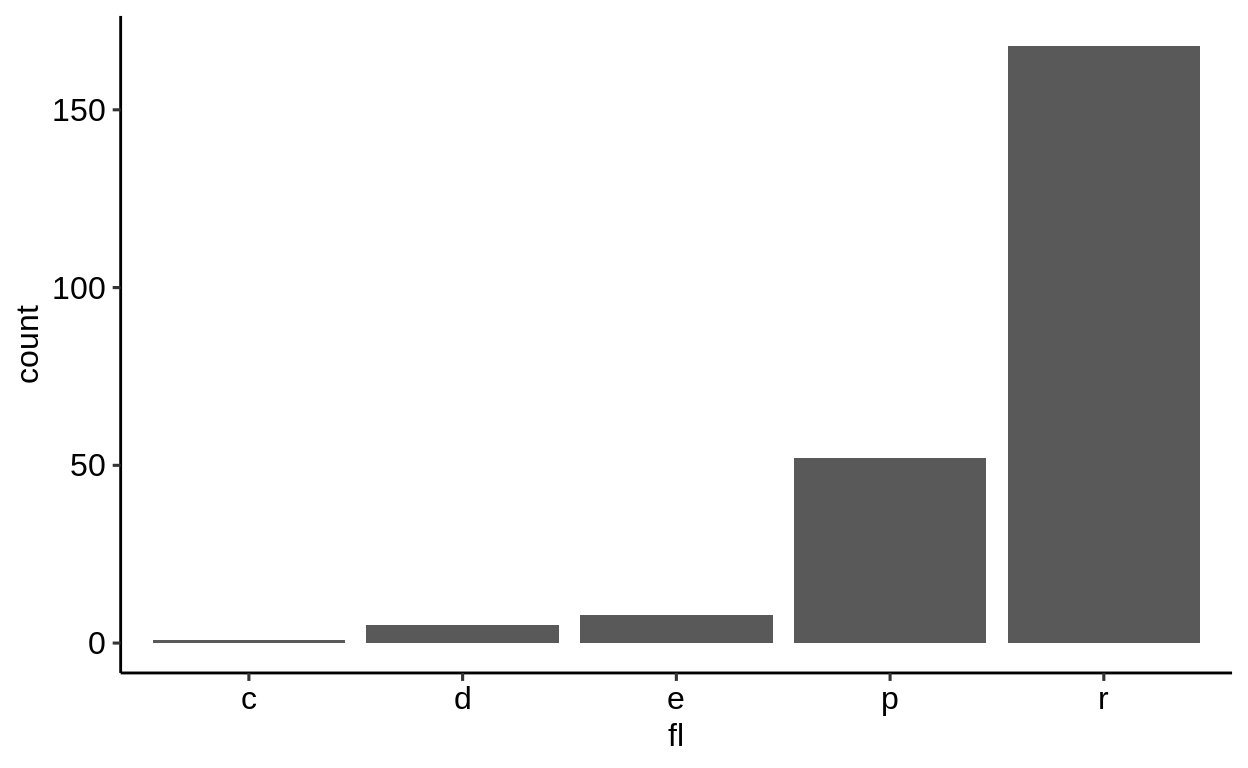
\includegraphics{vistransrep_files/figure-latex/14-example-for-discrete-var-barplot-1} \end{flushright}

\textbf{Exercises}

\begin{Shaded}
\begin{Highlighting}[]
\KeywordTok{browseURL}\NormalTok{(}\StringTok{"https://krlmlr.github.io/vistransrep/2019-11-zhr/scatter.html"}\NormalTok{)}
\end{Highlighting}
\end{Shaded}

\hypertarget{colors-and-shape}{%
\section{Colors and shape}\label{colors-and-shape}}

\emph{Click here to show setup code.}

\begin{Shaded}
\begin{Highlighting}[]
\KeywordTok{library}\NormalTok{(tidyverse)}
\end{Highlighting}
\end{Shaded}

\hypertarget{static-colors}{%
\subsection{Static colors}\label{static-colors}}

There are many ways to set a color for a specific geom.
The simplest is to set all observations of a geom to a dedicated color, supplied as a character value.

\begin{Shaded}
\begin{Highlighting}[]
\KeywordTok{ggplot}\NormalTok{(}
  \DataTypeTok{data =}\NormalTok{ mpg,}
  \DataTypeTok{mapping =} \KeywordTok{aes}\NormalTok{(}\DataTypeTok{x =}\NormalTok{ displ, }\DataTypeTok{y =}\NormalTok{ hwy)}
\NormalTok{) }\OperatorTok{+}
\StringTok{  }\KeywordTok{geom_point}\NormalTok{(}
    \DataTypeTok{color =} \StringTok{"blue"}
\NormalTok{  )}
\end{Highlighting}
\end{Shaded}

\begin{flushright}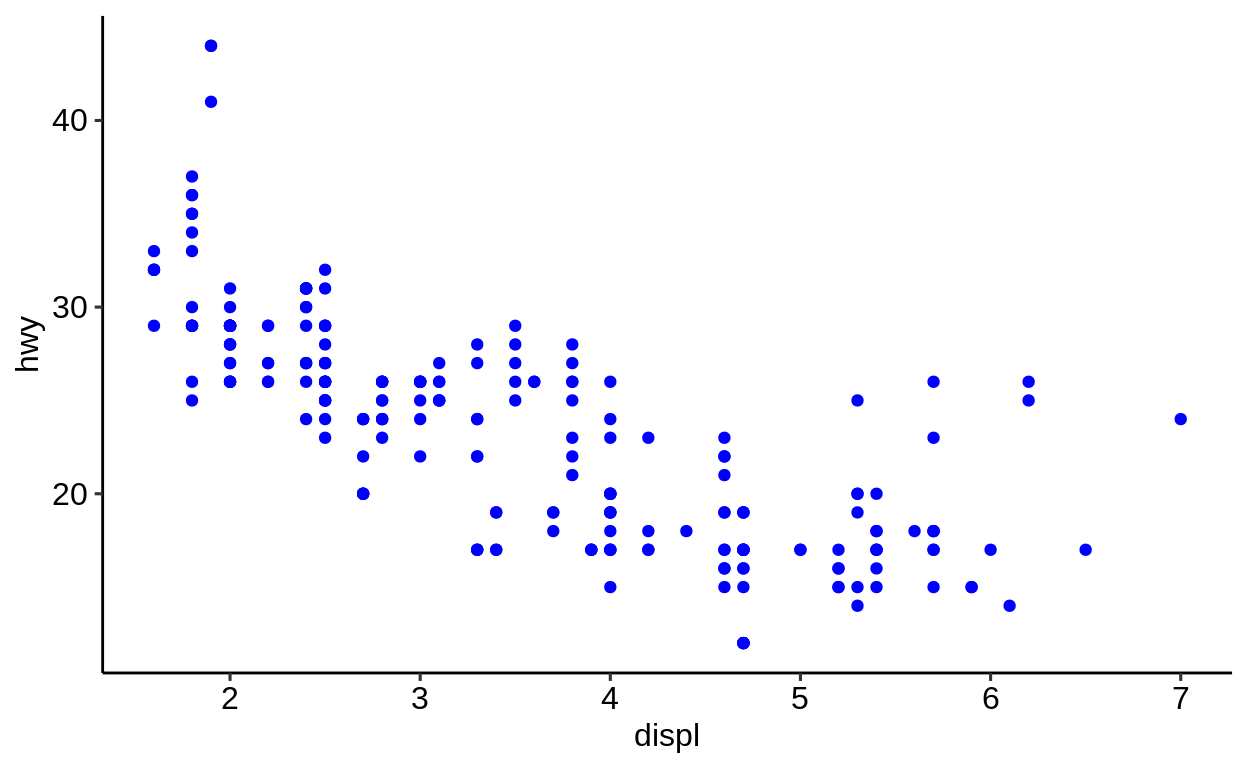
\includegraphics{vistransrep_files/figure-latex/105-static-color-blue-1} \end{flushright}

\hypertarget{dynamic-colors}{%
\subsection{Dynamic colors}\label{dynamic-colors}}

Dynamic colors, which depend on a variable of the dataset, need to be passed within an \texttt{aes()} call.
A direct specification like in the example above with \texttt{color\ =\ "blue"} only works for static colors.

\emph{Good to know}: While it is possible to include \texttt{color\ =\ class} directly in the \texttt{aes()} call of the \texttt{ggplot()} function, it is recommended to set it within the particular geom.
This is for two reasons:

\begin{itemize}
\tightlist
\item
  When working with multiple geoms, you can use different mappings for each geom without any possibility of conflicts
\item
  When reading the code, it becomes more clear which settings apply to which geoms
\end{itemize}

\textbf{Discrete}

Different colors can be mapped to the values of a variable by supplying a variable of the dataset.
The \texttt{class} variable is discrete and leads to a discrete color scale.

\begin{Shaded}
\begin{Highlighting}[]
\KeywordTok{ggplot}\NormalTok{(}
  \DataTypeTok{data =}\NormalTok{ mpg,}
  \DataTypeTok{mapping =} \KeywordTok{aes}\NormalTok{(}\DataTypeTok{x =}\NormalTok{ displ, }\DataTypeTok{y =}\NormalTok{ hwy)}
\NormalTok{) }\OperatorTok{+}
\StringTok{  }\KeywordTok{geom_point}\NormalTok{(}\KeywordTok{aes}\NormalTok{(}\DataTypeTok{color =}\NormalTok{ class))}
\end{Highlighting}
\end{Shaded}

\begin{flushright}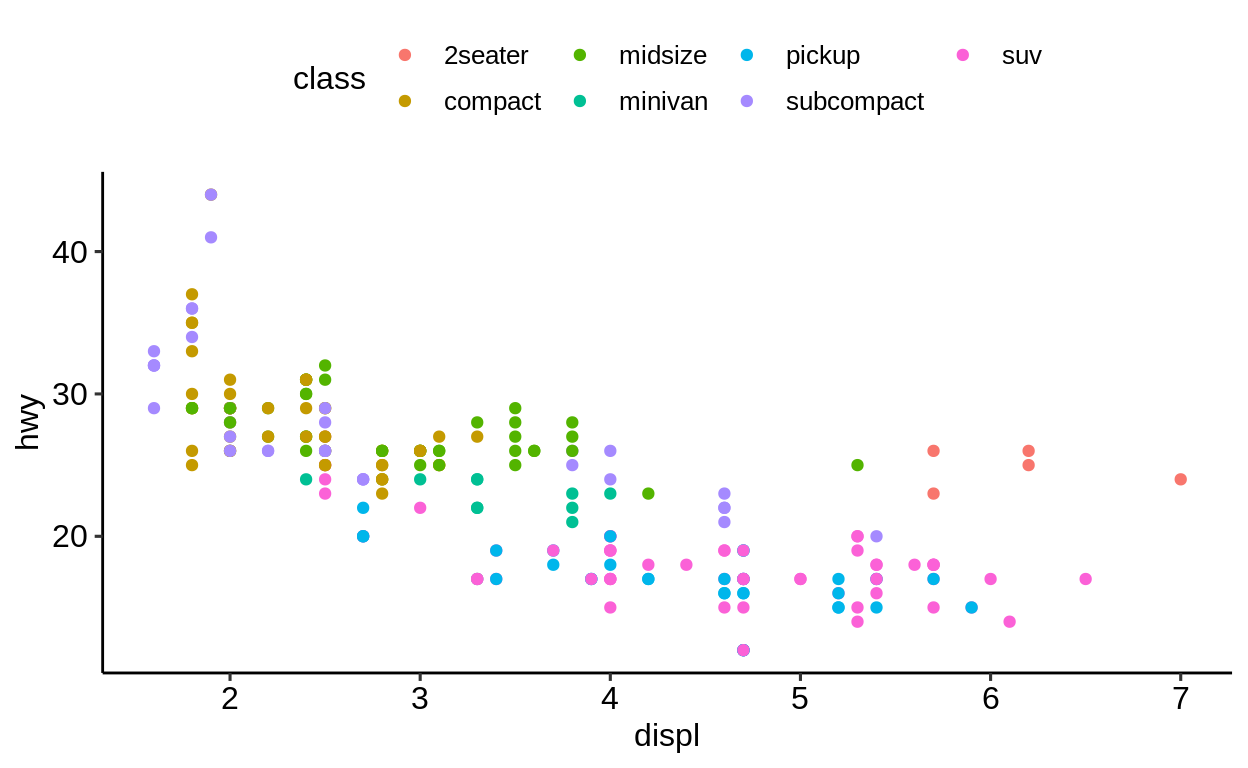
\includegraphics{vistransrep_files/figure-latex/105-dynamic-color-variable-mapping-discrete-1} \end{flushright}

\textbf{Continuous}

The \texttt{cty} attribute is continuous, the color scale is adapted accordingly.

\begin{Shaded}
\begin{Highlighting}[]
\KeywordTok{ggplot}\NormalTok{(}
  \DataTypeTok{data =}\NormalTok{ mpg,}
  \DataTypeTok{mapping =} \KeywordTok{aes}\NormalTok{(}\DataTypeTok{x =}\NormalTok{ displ, }\DataTypeTok{y =}\NormalTok{ hwy)}
\NormalTok{) }\OperatorTok{+}
\StringTok{  }\KeywordTok{geom_point}\NormalTok{(}\KeywordTok{aes}\NormalTok{(}\DataTypeTok{color =}\NormalTok{ cty))}
\end{Highlighting}
\end{Shaded}

\begin{flushright}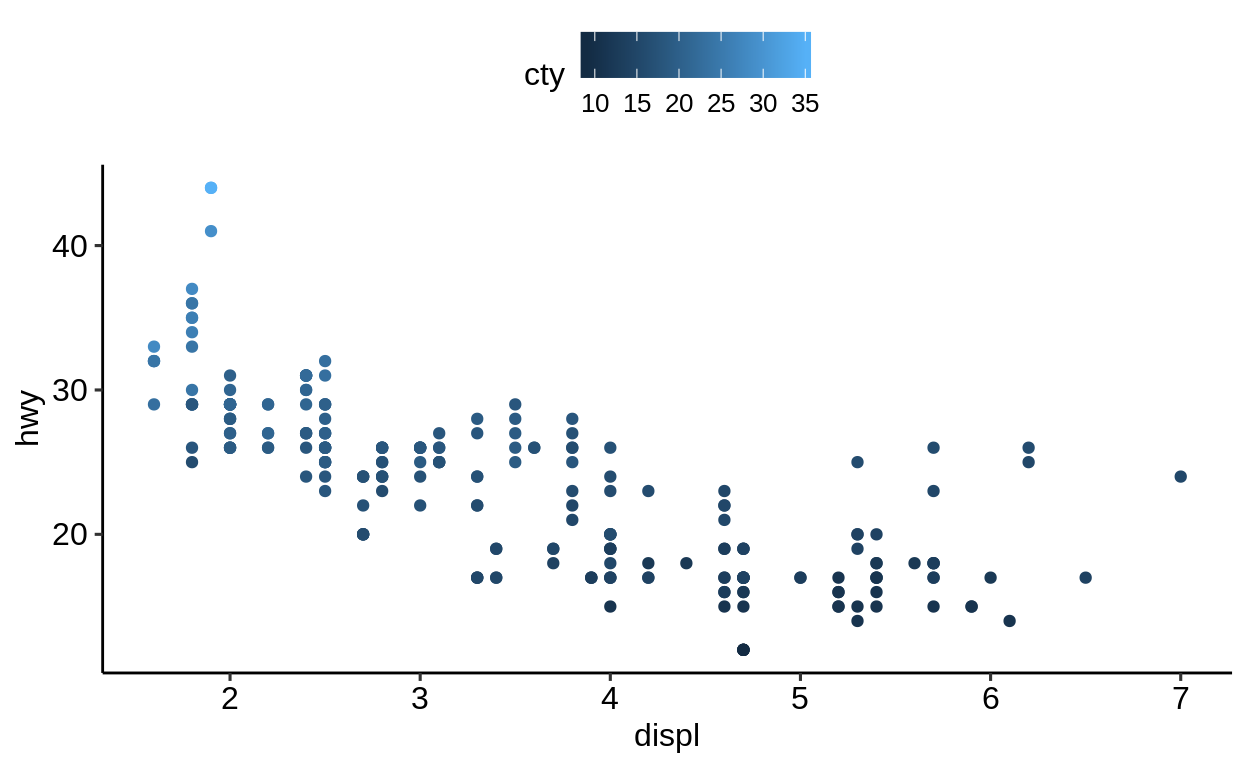
\includegraphics{vistransrep_files/figure-latex/105-dynamic-color-variable-mapping-cont-1} \end{flushright}

\hypertarget{shape}{%
\subsection{Shape}\label{shape}}

One more degree of freedom is the shape of the symbols to be plotted.

\begin{Shaded}
\begin{Highlighting}[]
\KeywordTok{ggplot}\NormalTok{(}
  \DataTypeTok{data =}\NormalTok{ mpg,}
  \DataTypeTok{mapping =} \KeywordTok{aes}\NormalTok{(}
    \DataTypeTok{x =}\NormalTok{ displ,}
    \DataTypeTok{y =}\NormalTok{ hwy}
\NormalTok{  )}
\NormalTok{) }\OperatorTok{+}
\StringTok{  }\KeywordTok{geom_point}\NormalTok{(}\KeywordTok{aes}\NormalTok{(}\DataTypeTok{shape =}\NormalTok{ fl))}
\end{Highlighting}
\end{Shaded}

\begin{flushright}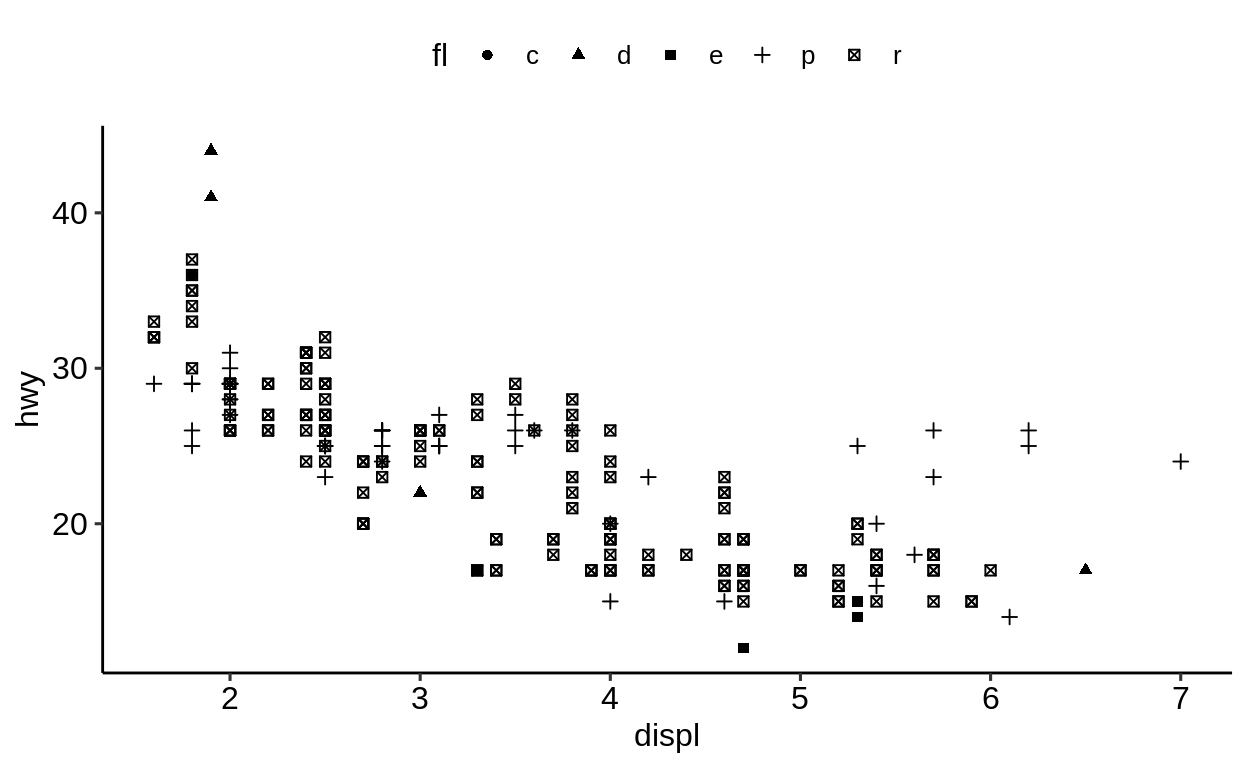
\includegraphics{vistransrep_files/figure-latex/105-shape-1} \end{flushright}

\hypertarget{combining-color-and-shape}{%
\subsection{Combining color and shape}\label{combining-color-and-shape}}

Color and shape can be combined.

\begin{Shaded}
\begin{Highlighting}[]
\KeywordTok{ggplot}\NormalTok{(}
  \DataTypeTok{data =}\NormalTok{ mpg,}
  \DataTypeTok{mapping =} \KeywordTok{aes}\NormalTok{(}
    \DataTypeTok{x =}\NormalTok{ displ,}
    \DataTypeTok{y =}\NormalTok{ hwy,}
\NormalTok{  )}
\NormalTok{) }\OperatorTok{+}
\StringTok{  }\KeywordTok{geom_point}\NormalTok{(}\KeywordTok{aes}\NormalTok{(}\DataTypeTok{color =}\NormalTok{ class, }\DataTypeTok{shape =}\NormalTok{ drv))}
\end{Highlighting}
\end{Shaded}

\begin{flushright}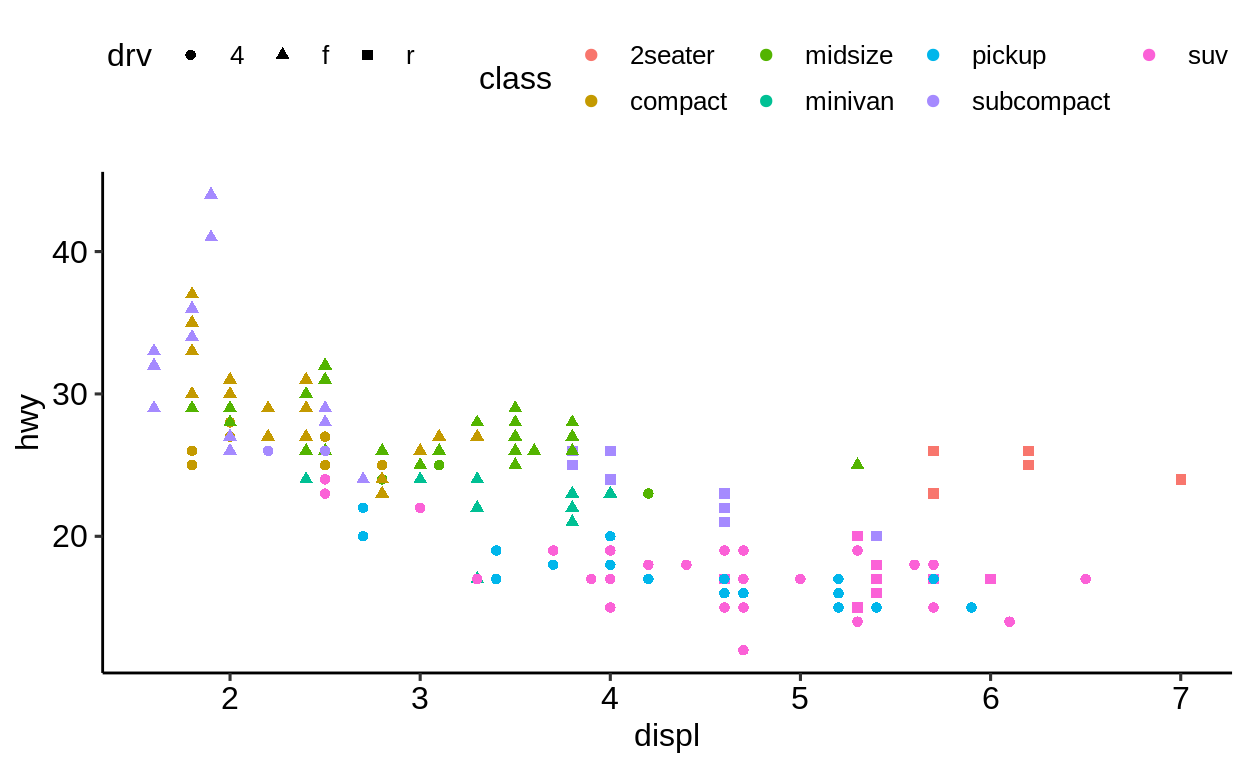
\includegraphics{vistransrep_files/figure-latex/105-dynamic-combining-color-and-shape-1} \end{flushright}

And last but not least, the size of the plotted symbols can be linked to numeric values of the mapped variable.

\begin{Shaded}
\begin{Highlighting}[]
\KeywordTok{ggplot}\NormalTok{(}
  \DataTypeTok{data =}\NormalTok{ mpg,}
  \DataTypeTok{mapping =} \KeywordTok{aes}\NormalTok{(}
    \DataTypeTok{x =}\NormalTok{ displ,}
    \DataTypeTok{y =}\NormalTok{ hwy}
\NormalTok{  )}
\NormalTok{) }\OperatorTok{+}
\StringTok{  }\KeywordTok{geom_point}\NormalTok{(}\KeywordTok{aes}\NormalTok{(}\DataTypeTok{size =}\NormalTok{ cty))}
\end{Highlighting}
\end{Shaded}

\begin{flushright}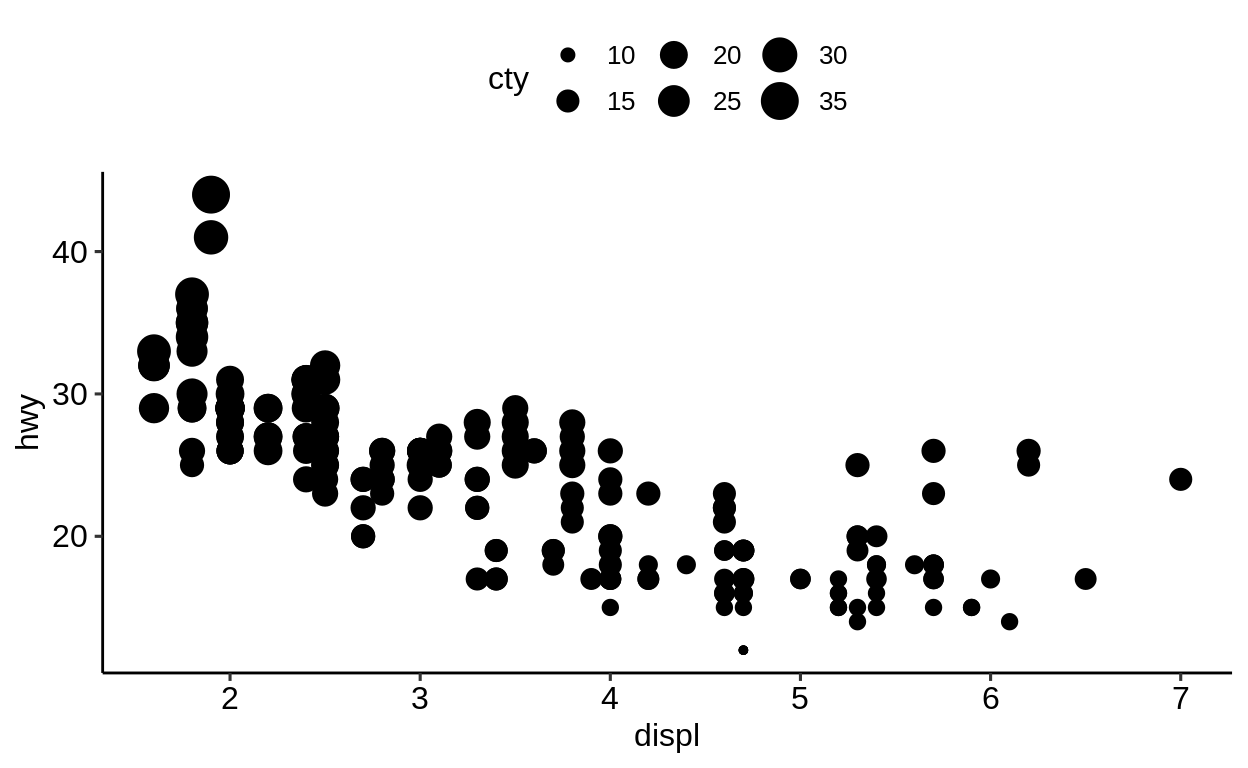
\includegraphics{vistransrep_files/figure-latex/105-dynamic-size-1} \end{flushright}

You can mix different aesthetic mappings in order to produce a plot with densely packed information.
However, be aware that adding too much information to a plot does not necessarily make it better.

\begin{Shaded}
\begin{Highlighting}[]
\KeywordTok{ggplot}\NormalTok{(}
  \DataTypeTok{data =}\NormalTok{ mpg,}
  \DataTypeTok{mapping =} \KeywordTok{aes}\NormalTok{(}
    \DataTypeTok{x =}\NormalTok{ displ,}
    \DataTypeTok{y =}\NormalTok{ hwy}
\NormalTok{  )}
\NormalTok{) }\OperatorTok{+}
\StringTok{  }\KeywordTok{geom_point}\NormalTok{(}\KeywordTok{aes}\NormalTok{(}
    \DataTypeTok{color =}\NormalTok{ class,}
    \DataTypeTok{size =}\NormalTok{ cty}
\NormalTok{  ))}
\end{Highlighting}
\end{Shaded}

\begin{flushright}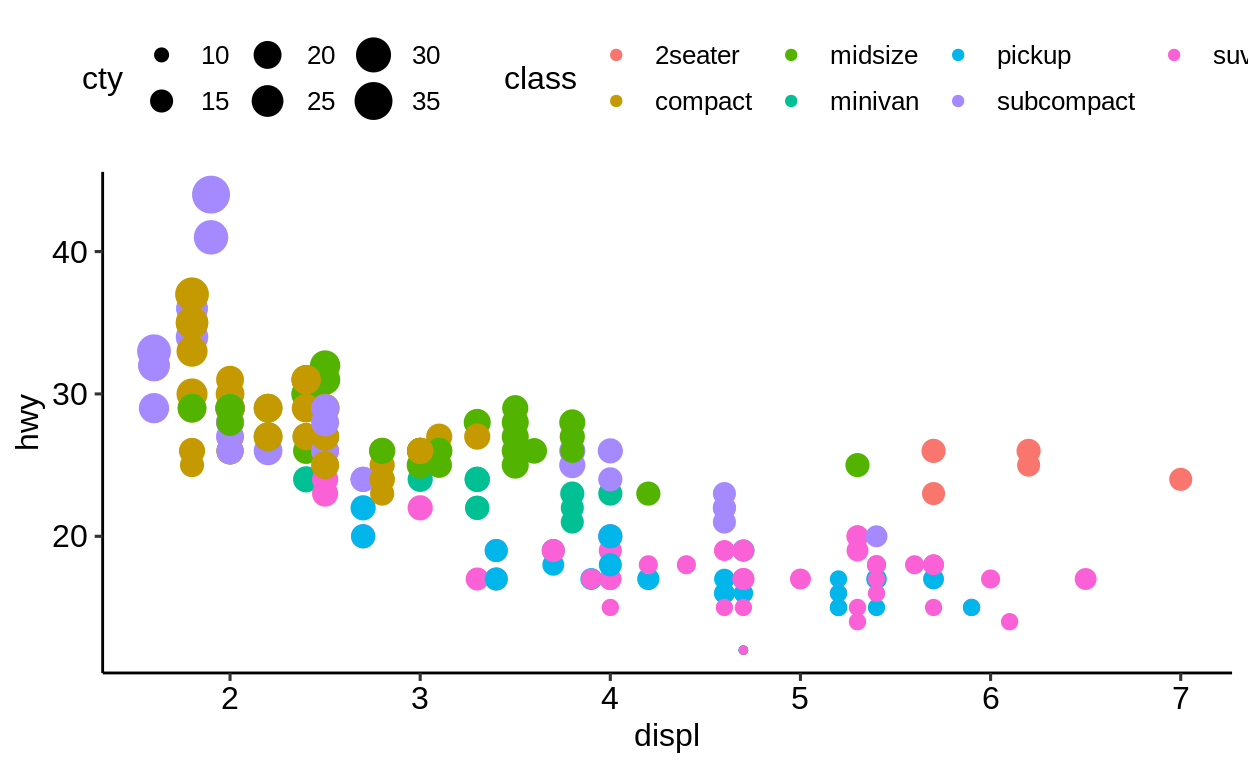
\includegraphics{vistransrep_files/figure-latex/105-sometimes-less-is-more-1} \end{flushright}

\hypertarget{transparency}{%
\subsection{Transparency}\label{transparency}}

Semi-transparency is another way to better display your data when observations are overlapping.
This is useful to get an impression of how many data points share the same coordinates.

\begin{Shaded}
\begin{Highlighting}[]
\KeywordTok{ggplot}\NormalTok{(}
  \DataTypeTok{data =}\NormalTok{ mpg,}
  \DataTypeTok{mapping =} \KeywordTok{aes}\NormalTok{(}
    \DataTypeTok{x =}\NormalTok{ displ,}
    \DataTypeTok{y =}\NormalTok{ hwy}
\NormalTok{  )}
\NormalTok{) }\OperatorTok{+}
\StringTok{  }\KeywordTok{geom_point}\NormalTok{(}\DataTypeTok{alpha =} \FloatTok{0.2}\NormalTok{)}
\end{Highlighting}
\end{Shaded}

\begin{flushright}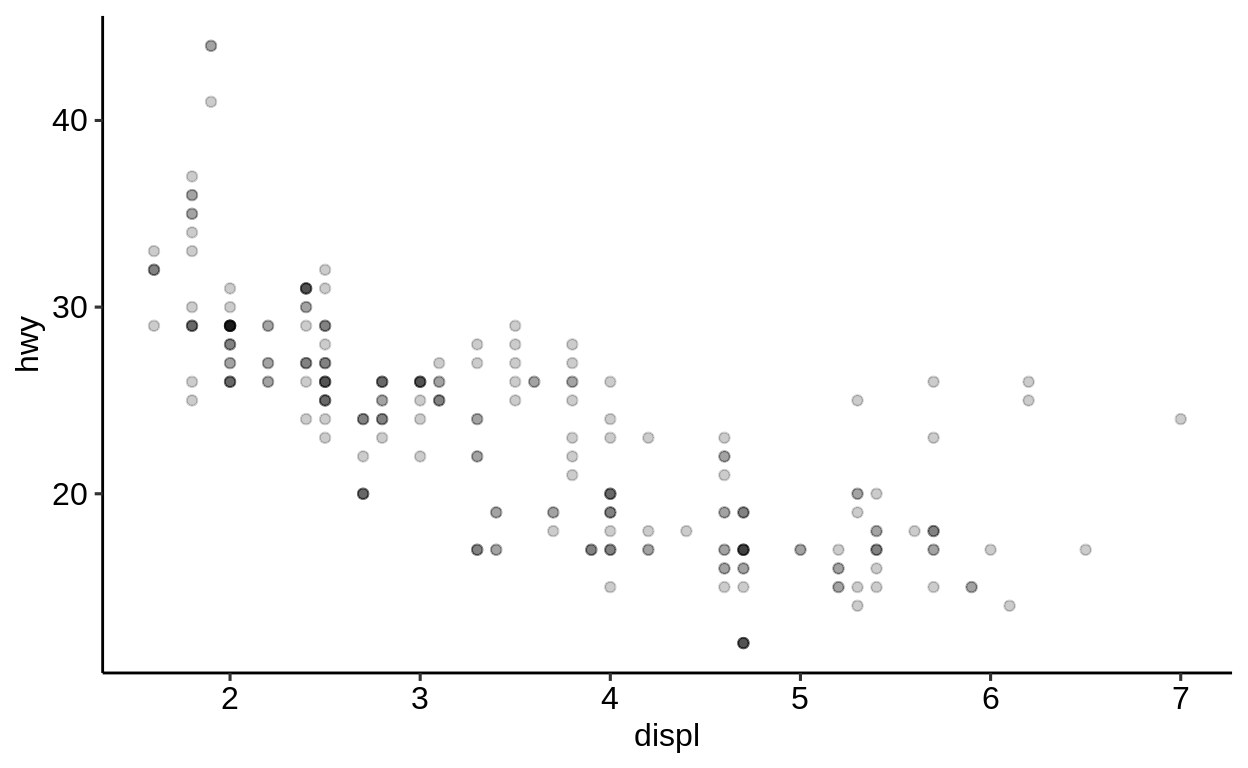
\includegraphics{vistransrep_files/figure-latex/105-transparency-alpha-1} \end{flushright}

\hypertarget{what-can-go-wrong}{%
\subsection{What can go wrong}\label{what-can-go-wrong}}

If you try to specify a color in the \texttt{mapping}-argument of the main \texttt{ggplot()} call, you will face an error since a mapping of a variable to an aesthetic is expected.

\begin{Shaded}
\begin{Highlighting}[]
\KeywordTok{try}\NormalTok{(}\KeywordTok{print}\NormalTok{(}
  \KeywordTok{ggplot}\NormalTok{(}
    \DataTypeTok{data =}\NormalTok{ mpg,}
    \DataTypeTok{mapping =} \KeywordTok{aes}\NormalTok{(}
      \DataTypeTok{x =}\NormalTok{ displ,}
      \DataTypeTok{y =}\NormalTok{ hwy,}
      \DataTypeTok{color =}\NormalTok{ blue}
\NormalTok{    )}
\NormalTok{  ) }\OperatorTok{+}
\StringTok{    }\KeywordTok{geom_point}\NormalTok{()}
\NormalTok{))}
\end{Highlighting}
\end{Shaded}

\begin{flushright}
\includegraphics{vistransrep_files/figure-latex/105-what-can-go-wrong-1} \end{flushright}

\begin{verbatim}
## Error in FUN(X[[i]], ...) : object 'blue' not found
\end{verbatim}

R treats objects without quotation marks in a special way, expecting them to be variables.
Since \texttt{blue} is not a variable of \texttt{mpg}, this did not work.
Use quotation marks if you mean a string, as opposed to a variable or object name.

\begin{Shaded}
\begin{Highlighting}[]
\NormalTok{mpg}
\end{Highlighting}
\end{Shaded}

\begin{verbatim}
## # A tibble: 234 x 11
##   manufacturer model displ  year   cyl trans drv     cty   hwy
##   <chr>        <chr> <dbl> <int> <int> <chr> <chr> <int> <int>
## 1 audi         a4      1.8  1999     4 auto~ f        18    29
## 2 audi         a4      1.8  1999     4 manu~ f        21    29
## 3 audi         a4      2    2008     4 manu~ f        20    31
## # ... with 231 more rows, and 2 more variables: fl <chr>,
## #   class <chr>
\end{verbatim}

\begin{Shaded}
\begin{Highlighting}[]
\StringTok{"mpg"}
\end{Highlighting}
\end{Shaded}

\begin{verbatim}
## [1] "mpg"
\end{verbatim}

So what if we pass the color as a character variable?

\begin{Shaded}
\begin{Highlighting}[]
\KeywordTok{ggplot}\NormalTok{(}
  \DataTypeTok{data =}\NormalTok{ mpg,}
  \DataTypeTok{mapping =} \KeywordTok{aes}\NormalTok{(}
    \DataTypeTok{x =}\NormalTok{ displ,}
    \DataTypeTok{y =}\NormalTok{ hwy}
\NormalTok{  )}
\NormalTok{) }\OperatorTok{+}
\StringTok{  }\KeywordTok{geom_point}\NormalTok{(}\KeywordTok{aes}\NormalTok{(}\DataTypeTok{color =} \StringTok{"blue"}\NormalTok{))}
\end{Highlighting}
\end{Shaded}

\begin{flushright}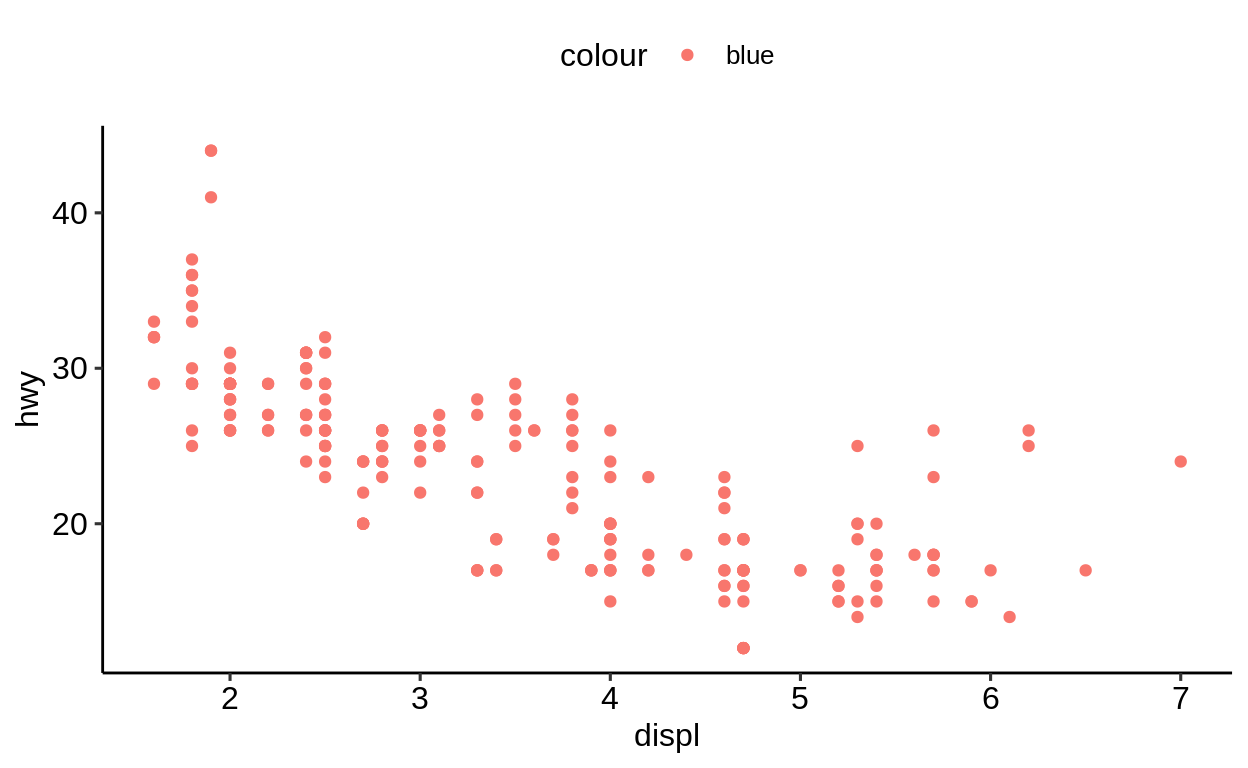
\includegraphics{vistransrep_files/figure-latex/105-what-happens-with-strings-in-aes-1} \end{flushright}

At least there was no error, but now the constant value \texttt{blue} is mapped to the first default color of the color mapping, which happens to be red.
We could have been fooled, if it had been blue.
Recall, it is best to specify geom related mappings with the respective geom function.

\begin{Shaded}
\begin{Highlighting}[]
\KeywordTok{ggplot}\NormalTok{(}
  \DataTypeTok{data =}\NormalTok{ mpg,}
  \DataTypeTok{mapping =} \KeywordTok{aes}\NormalTok{(}
    \DataTypeTok{x =}\NormalTok{ displ,}
    \DataTypeTok{y =}\NormalTok{ hwy}
\NormalTok{  )}
\NormalTok{) }\OperatorTok{+}
\StringTok{  }\KeywordTok{geom_point}\NormalTok{(}
    \DataTypeTok{color =} \StringTok{"blue"}
\NormalTok{  )}
\end{Highlighting}
\end{Shaded}

\begin{flushright}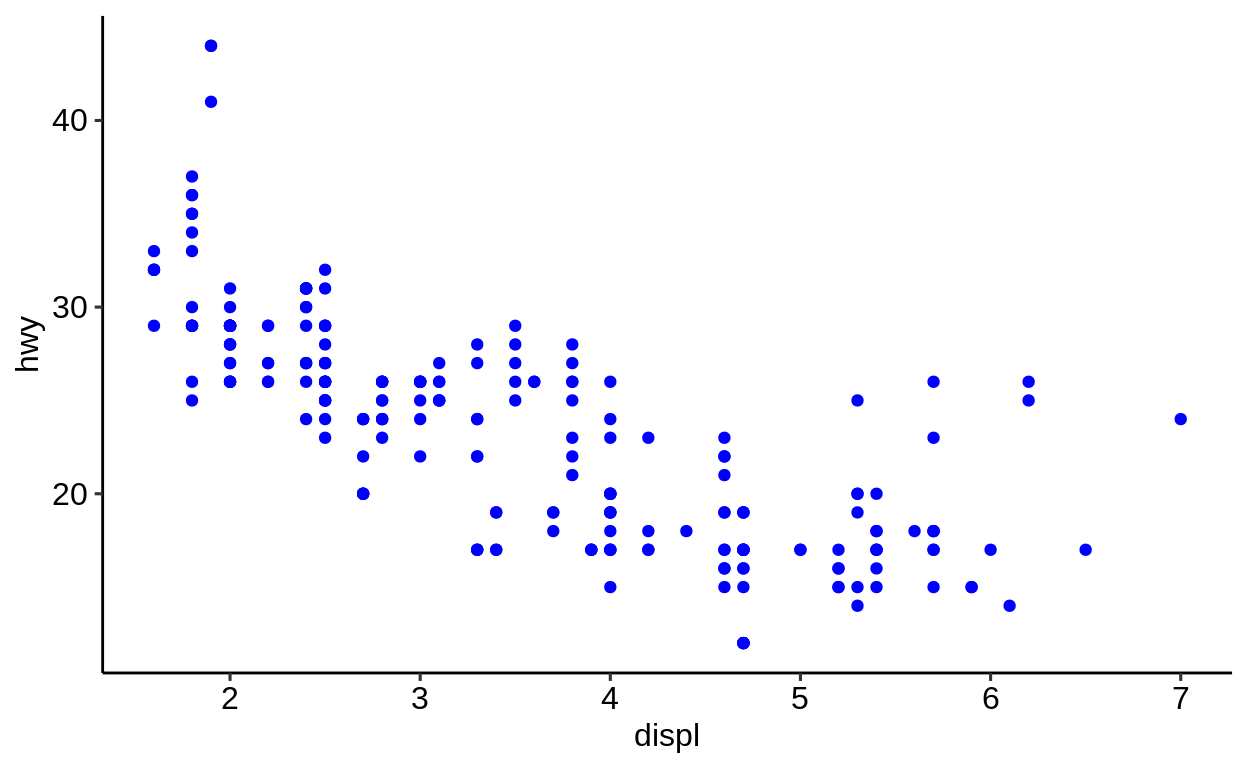
\includegraphics{vistransrep_files/figure-latex/105-map-static-colors-outside-of-aes-1} \end{flushright}

\textbf{Exercises}

\url{https://krlmlr.github.io/vistransrep/2019-11-zhr/scatter3.html}

\hypertarget{labels}{%
\section{Labels}\label{labels}}

\emph{Click here to show setup code.}

\begin{Shaded}
\begin{Highlighting}[]
\KeywordTok{library}\NormalTok{(tidyverse)}
\end{Highlighting}
\end{Shaded}

For character variables there is further way of integrating its value to a plot.
\texttt{geom\_text()} takes a \texttt{label} argument, which influences the plot in the following way.

\begin{Shaded}
\begin{Highlighting}[]
\KeywordTok{ggplot}\NormalTok{(}
  \DataTypeTok{data =}\NormalTok{ mpg,}
  \DataTypeTok{mapping =} \KeywordTok{aes}\NormalTok{(}\DataTypeTok{x =}\NormalTok{ displ, }\DataTypeTok{y =}\NormalTok{ hwy)}
\NormalTok{) }\OperatorTok{+}
\StringTok{  }\KeywordTok{geom_text}\NormalTok{(}\DataTypeTok{label =} \StringTok{"A"}\NormalTok{)}
\end{Highlighting}
\end{Shaded}

\begin{flushright}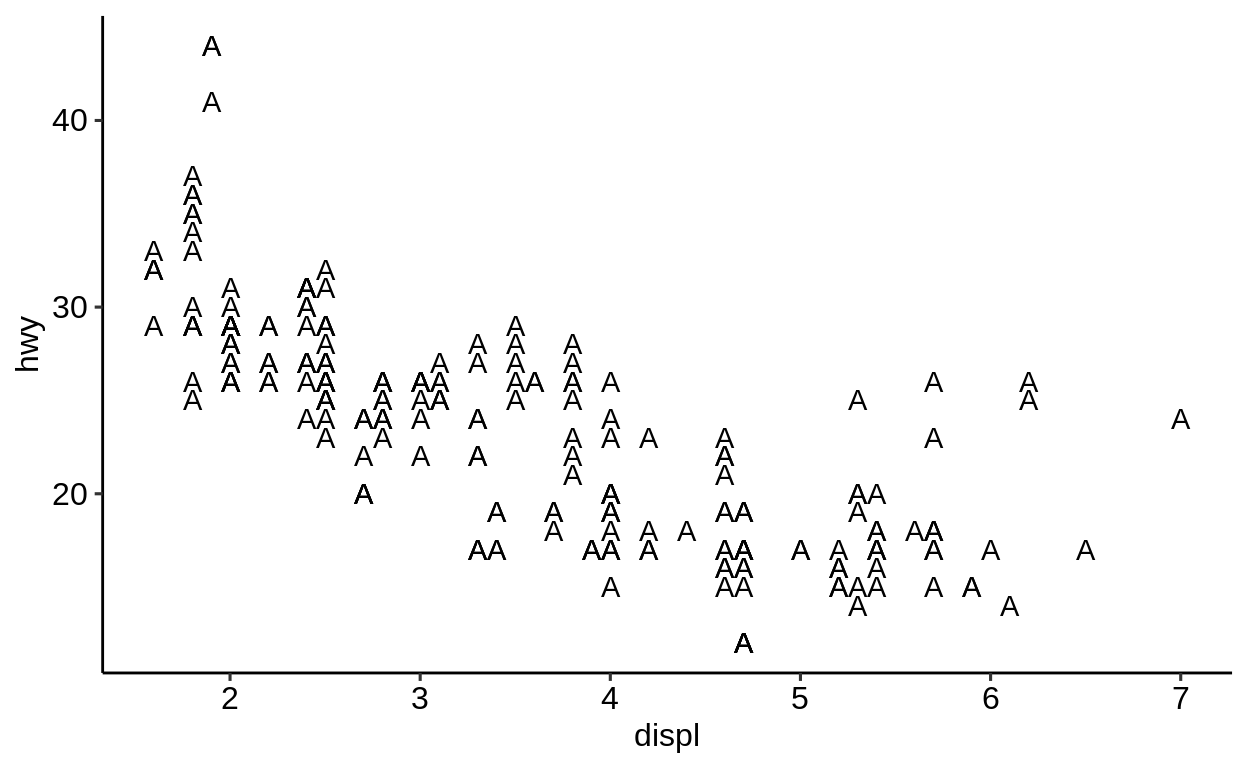
\includegraphics{vistransrep_files/figure-latex/16-showcase-geom-text-1} \end{flushright}

Let's try to map this argument to a variable (here: \texttt{drv}) of our dataset in the \texttt{mapping} argument of \texttt{ggplot()}.

\begin{Shaded}
\begin{Highlighting}[]
\KeywordTok{ggplot}\NormalTok{(}
  \DataTypeTok{data =}\NormalTok{ mpg,}
  \DataTypeTok{mapping =} \KeywordTok{aes}\NormalTok{(}\DataTypeTok{x =}\NormalTok{ displ, }\DataTypeTok{y =}\NormalTok{ hwy)}
\NormalTok{) }\OperatorTok{+}
\StringTok{  }\KeywordTok{geom_text}\NormalTok{(}\DataTypeTok{label =} \StringTok{"drv"}\NormalTok{)}
\end{Highlighting}
\end{Shaded}

\begin{flushright}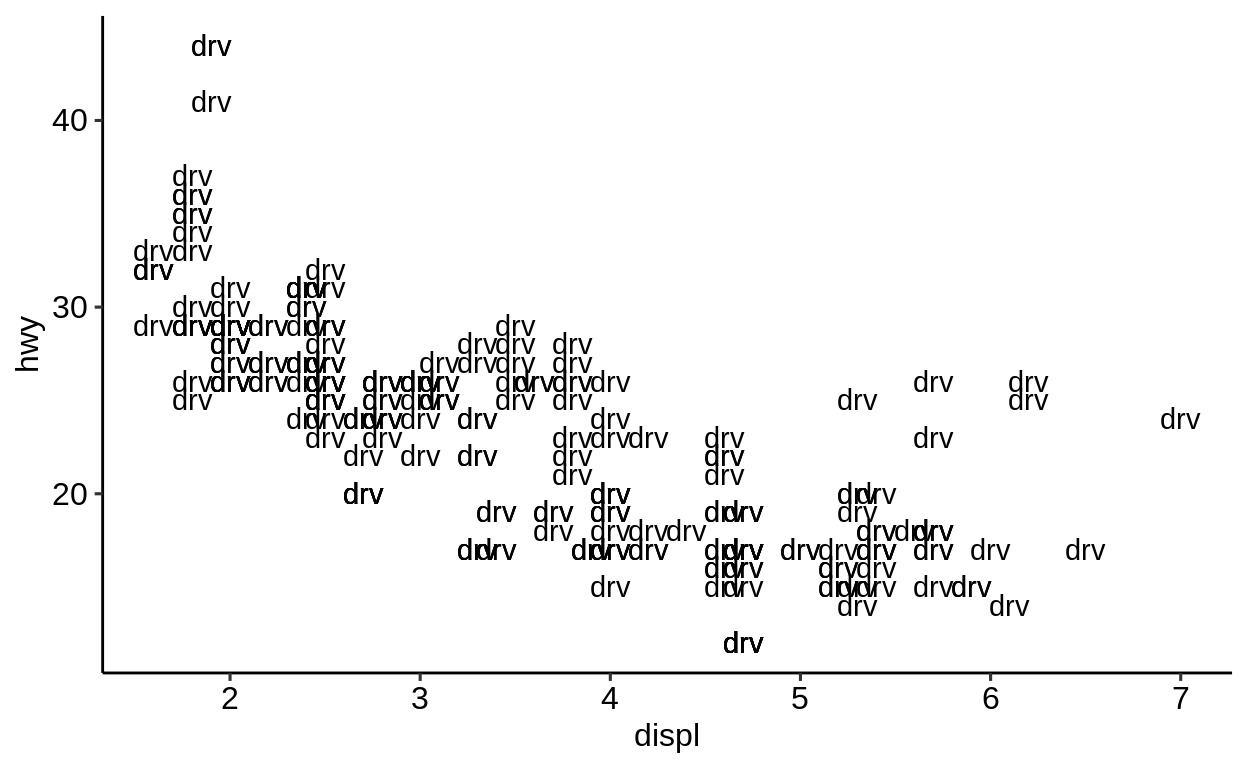
\includegraphics{vistransrep_files/figure-latex/16-object-vs-string-again-1} \end{flushright}

Right, of course we need to pass the variable without quotation marks, otherwise it is interpreted as a (constant) character variable.
When changing this, a vector with the values of the variable is passed on to \texttt{geom\_text()}.
This is one way of including the values of character variables in a plot.

\begin{Shaded}
\begin{Highlighting}[]
\KeywordTok{ggplot}\NormalTok{(}
  \DataTypeTok{data =}\NormalTok{ mpg,}
  \DataTypeTok{mapping =} \KeywordTok{aes}\NormalTok{(}\DataTypeTok{x =}\NormalTok{ displ, }\DataTypeTok{y =}\NormalTok{ hwy)}
\NormalTok{) }\OperatorTok{+}
\StringTok{  }\KeywordTok{geom_text}\NormalTok{(}\KeywordTok{aes}\NormalTok{(}\DataTypeTok{label =}\NormalTok{ drv))}
\end{Highlighting}
\end{Shaded}

\begin{flushright}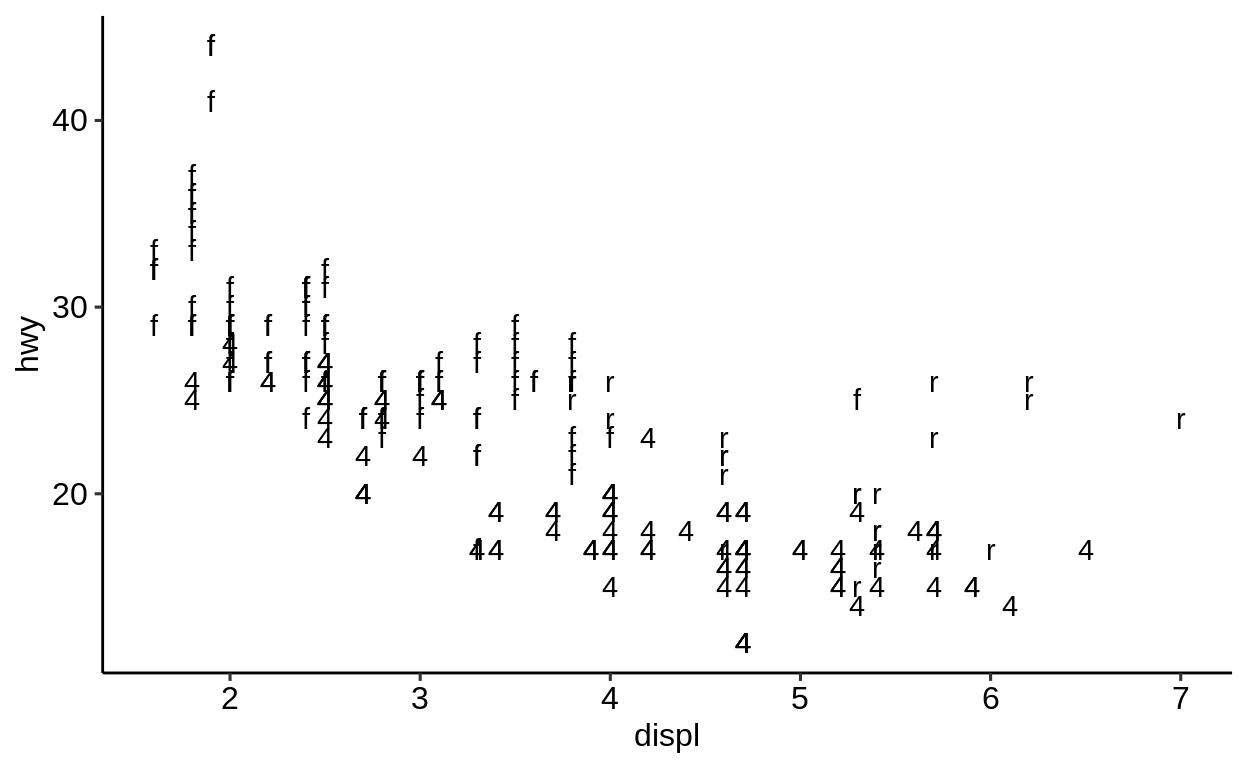
\includegraphics{vistransrep_files/figure-latex/16-dynamic-labeling-to-variable-1} \end{flushright}

When adding more than one \texttt{geom()}-function, multiple geometries are added to the plot.
However, because \texttt{geom\_point()} has no support for passing a label, we can only use this mapping in \texttt{geom\_text()}.

\begin{Shaded}
\begin{Highlighting}[]
\KeywordTok{ggplot}\NormalTok{(}
  \DataTypeTok{data =}\NormalTok{ mpg,}
  \DataTypeTok{mapping =} \KeywordTok{aes}\NormalTok{(}\DataTypeTok{x =}\NormalTok{ displ, }\DataTypeTok{y =}\NormalTok{ hwy)}
\NormalTok{) }\OperatorTok{+}
\StringTok{  }\KeywordTok{geom_point}\NormalTok{() }\OperatorTok{+}
\StringTok{  }\KeywordTok{geom_text}\NormalTok{(}\KeywordTok{aes}\NormalTok{(}\DataTypeTok{label =}\NormalTok{ drv))}
\end{Highlighting}
\end{Shaded}

\begin{flushright}\includegraphics{vistransrep_files/figure-latex/16-points-and-labels-overplotting-1} \end{flushright}

Since this looks just slightly odd, let's try to make it more apparent, what is happening.

\begin{Shaded}
\begin{Highlighting}[]
\KeywordTok{ggplot}\NormalTok{(}
  \DataTypeTok{data =}\NormalTok{ mpg,}
  \DataTypeTok{mapping =} \KeywordTok{aes}\NormalTok{(}\DataTypeTok{x =}\NormalTok{ displ, }\DataTypeTok{y =}\NormalTok{ hwy)}
\NormalTok{) }\OperatorTok{+}
\StringTok{  }\KeywordTok{geom_point}\NormalTok{(}\DataTypeTok{color =} \StringTok{"blue"}\NormalTok{) }\OperatorTok{+}
\StringTok{  }\KeywordTok{geom_text}\NormalTok{(}\KeywordTok{aes}\NormalTok{(}\DataTypeTok{label =}\NormalTok{ drv), }\DataTypeTok{size =} \DecValTok{10}\NormalTok{)}
\end{Highlighting}
\end{Shaded}

\begin{flushright}\includegraphics{vistransrep_files/figure-latex/16-aesthetic-changes-to-distinguish-better-1} \end{flushright}

\hypertarget{themes}{%
\section{Themes}\label{themes}}

\emph{Click here to show setup code.}

\begin{Shaded}
\begin{Highlighting}[]
\KeywordTok{library}\NormalTok{(tidyverse)}
\end{Highlighting}
\end{Shaded}

In this section we are looking at the use of visual themes to easily change the look and feel of a plot.
We start with the introduction of the default theme -- \texttt{theme\_grey()} function.

\begin{Shaded}
\begin{Highlighting}[]
\KeywordTok{ggplot}\NormalTok{(}
  \DataTypeTok{data =}\NormalTok{ mpg,}
  \DataTypeTok{mapping =} \KeywordTok{aes}\NormalTok{(}\DataTypeTok{x =}\NormalTok{ displ, }\DataTypeTok{y =}\NormalTok{ hwy)}
\NormalTok{) }\OperatorTok{+}
\StringTok{  }\KeywordTok{geom_point}\NormalTok{() }\OperatorTok{+}
\StringTok{  }\KeywordTok{theme_grey}\NormalTok{()}
\end{Highlighting}
\end{Shaded}

\begin{flushright}\includegraphics{vistransrep_files/figure-latex/17-base-plot-with-default-theme-1} \end{flushright}

Change the default \texttt{theme\_grey()} to a more traditional black-and-white theme:

\begin{Shaded}
\begin{Highlighting}[]
\KeywordTok{ggplot}\NormalTok{(}
  \DataTypeTok{data =}\NormalTok{ mpg,}
  \DataTypeTok{mapping =} \KeywordTok{aes}\NormalTok{(}\DataTypeTok{x =}\NormalTok{ displ, }\DataTypeTok{y =}\NormalTok{ hwy)}
\NormalTok{) }\OperatorTok{+}
\StringTok{  }\KeywordTok{geom_point}\NormalTok{() }\OperatorTok{+}
\StringTok{  }\KeywordTok{theme_bw}\NormalTok{()}
\end{Highlighting}
\end{Shaded}

\begin{flushright}\includegraphics{vistransrep_files/figure-latex/17-bw-theme-1} \end{flushright}

Also in this scheme the color aesthetic works as it normally does.
The black-and-whiteness only relates to the background.

\begin{Shaded}
\begin{Highlighting}[]
\KeywordTok{ggplot}\NormalTok{(}
  \DataTypeTok{data =}\NormalTok{ mpg,}
  \DataTypeTok{mapping =} \KeywordTok{aes}\NormalTok{(}\DataTypeTok{x =}\NormalTok{ displ, }\DataTypeTok{y =}\NormalTok{ hwy)}
\NormalTok{) }\OperatorTok{+}
\StringTok{  }\KeywordTok{geom_point}\NormalTok{(}\KeywordTok{aes}\NormalTok{(}\DataTypeTok{color =}\NormalTok{ class)) }\OperatorTok{+}
\StringTok{  }\KeywordTok{theme_bw}\NormalTok{()}
\end{Highlighting}
\end{Shaded}

\begin{flushright}\includegraphics{vistransrep_files/figure-latex/17-theme-does-not-affect-color-palette-of-geoms-1} \end{flushright}

Calling the function \texttt{theme()} after a \texttt{theme\_...()} call let's you tweak certain aspects of the theme.

Some plots work better with the legend at the bottom.

\begin{Shaded}
\begin{Highlighting}[]
\KeywordTok{ggplot}\NormalTok{(}
  \DataTypeTok{data =}\NormalTok{ mpg,}
  \DataTypeTok{mapping =} \KeywordTok{aes}\NormalTok{(}\DataTypeTok{x =}\NormalTok{ displ, }\DataTypeTok{y =}\NormalTok{ hwy)}
\NormalTok{) }\OperatorTok{+}
\StringTok{  }\KeywordTok{geom_point}\NormalTok{(}\KeywordTok{aes}\NormalTok{(}\DataTypeTok{color =}\NormalTok{ class)) }\OperatorTok{+}
\StringTok{  }\KeywordTok{theme_bw}\NormalTok{() }\OperatorTok{+}
\StringTok{  }\KeywordTok{theme}\NormalTok{(}\DataTypeTok{legend.position =} \StringTok{"bottom"}\NormalTok{)}
\end{Highlighting}
\end{Shaded}

\begin{flushright}\includegraphics{vistransrep_files/figure-latex/17-occasionally-useful-legend-at-the-bottom-1} \end{flushright}

Mind that \texttt{theme\_...()} functions overwrite all previous settings of \texttt{theme()}:

\begin{Shaded}
\begin{Highlighting}[]
\KeywordTok{ggplot}\NormalTok{(}
  \DataTypeTok{data =}\NormalTok{ mpg,}
  \DataTypeTok{mapping =} \KeywordTok{aes}\NormalTok{(}\DataTypeTok{x =}\NormalTok{ displ, }\DataTypeTok{y =}\NormalTok{ hwy)}
\NormalTok{) }\OperatorTok{+}
\StringTok{  }\KeywordTok{geom_point}\NormalTok{(}\KeywordTok{aes}\NormalTok{(}\DataTypeTok{color =}\NormalTok{ class)) }\OperatorTok{+}
\StringTok{  }\KeywordTok{theme}\NormalTok{(}\DataTypeTok{legend.position =} \StringTok{"bottom"}\NormalTok{) }\OperatorTok{+}
\StringTok{  }\KeywordTok{theme_bw}\NormalTok{()}
\end{Highlighting}
\end{Shaded}

\begin{flushright}\includegraphics{vistransrep_files/figure-latex/17-theme-overwrites-theme-calls-mind-the-order-1} \end{flushright}

The first argument of each \texttt{theme\_...()} function is \texttt{base\_size}, which refers to the font size of all elements in the plot.

\begin{Shaded}
\begin{Highlighting}[]
\KeywordTok{ggplot}\NormalTok{(}
  \DataTypeTok{data =}\NormalTok{ mpg,}
  \DataTypeTok{mapping =} \KeywordTok{aes}\NormalTok{(}\DataTypeTok{x =}\NormalTok{ displ, }\DataTypeTok{y =}\NormalTok{ hwy, }\DataTypeTok{color =}\NormalTok{ class)}
\NormalTok{) }\OperatorTok{+}
\StringTok{  }\KeywordTok{geom_point}\NormalTok{() }\OperatorTok{+}
\StringTok{  }\KeywordTok{theme_bw}\NormalTok{(}\DecValTok{16}\NormalTok{)}
\end{Highlighting}
\end{Shaded}

\begin{flushright}\includegraphics{vistransrep_files/figure-latex/17-first-param-of-theme-functions-is-base-size-1} \end{flushright}

If we were asked to suggest themes, we'd go for

\begin{itemize}
\tightlist
\item
  \texttt{ggplot2::theme\_minimal()}
\item
  \texttt{hrbrthemes::theme\_ipsum()}
\item
  \texttt{ggpubr::theme\_pubr()}
\end{itemize}

Here is how \texttt{ggpubr::theme\_pubr()} looks like.

\begin{Shaded}
\begin{Highlighting}[]
\KeywordTok{ggplot}\NormalTok{(}
  \DataTypeTok{data =}\NormalTok{ mpg,}
  \DataTypeTok{mapping =} \KeywordTok{aes}\NormalTok{(}\DataTypeTok{x =}\NormalTok{ displ, }\DataTypeTok{y =}\NormalTok{ hwy, }\DataTypeTok{color =}\NormalTok{ class)}
\NormalTok{) }\OperatorTok{+}
\StringTok{  }\KeywordTok{geom_point}\NormalTok{() }\OperatorTok{+}
\StringTok{  }\NormalTok{ggpubr}\OperatorTok{::}\KeywordTok{theme_pubr}\NormalTok{()}
\end{Highlighting}
\end{Shaded}

\begin{flushright}\includegraphics{vistransrep_files/figure-latex/17-predefined-custom-themes-available-e-g-in-ggpubr-package-1} \end{flushright}

Also from here onward we will use \texttt{theme\_pubr()} as the default theme for plots.
This can be done by setting

\hypertarget{scales}{%
\section{Scales}\label{scales}}

\emph{Click here to show setup code.}

\begin{Shaded}
\begin{Highlighting}[]
\KeywordTok{library}\NormalTok{(tidyverse)}
\KeywordTok{library}\NormalTok{(ggpubr)}
\end{Highlighting}
\end{Shaded}

\begin{verbatim}
## Loading required package: magrittr
\end{verbatim}

\begin{verbatim}
## 
## Attaching package: 'magrittr'
\end{verbatim}

\begin{verbatim}
## The following object is masked from 'package:purrr':
## 
##     set_names
\end{verbatim}

\begin{verbatim}
## The following object is masked from 'package:tidyr':
## 
##     extract
\end{verbatim}

\begin{Shaded}
\begin{Highlighting}[]
\KeywordTok{theme_set}\NormalTok{(}\KeywordTok{theme_pubr}\NormalTok{())}
\end{Highlighting}
\end{Shaded}

In this section we want to spend some time getting to know how to customize the labels and scales of plots using \{ggplot2\}.
We start with a pretty basic plot using the \texttt{mpg}-tibble which comes with the \{tidyverse\}.

\begin{Shaded}
\begin{Highlighting}[]
\KeywordTok{ggplot}\NormalTok{(}
  \DataTypeTok{data =}\NormalTok{ mpg,}
  \DataTypeTok{mapping =} \KeywordTok{aes}\NormalTok{(}\DataTypeTok{x =}\NormalTok{ displ, }\DataTypeTok{y =}\NormalTok{ hwy, }\DataTypeTok{color =}\NormalTok{ class)}
\NormalTok{) }\OperatorTok{+}
\StringTok{  }\KeywordTok{geom_point}\NormalTok{()}
\end{Highlighting}
\end{Shaded}

\begin{flushright}\includegraphics{vistransrep_files/figure-latex/108-base-plot-to-start-with-1} \end{flushright}

\hypertarget{labs}{%
\subsection{\texorpdfstring{\texttt{labs()}}{labs()}}\label{labs}}

With \texttt{labs()} you can label all sorts of aesthetics (axes, color mapping, \ldots{}).
Additionally you can set the title/subtitle and also add a caption and a tag.

\begin{Shaded}
\begin{Highlighting}[]
\KeywordTok{ggplot}\NormalTok{(}
  \DataTypeTok{data =}\NormalTok{ mpg,}
  \DataTypeTok{mapping =} \KeywordTok{aes}\NormalTok{(}\DataTypeTok{x =}\NormalTok{ displ, }\DataTypeTok{y =}\NormalTok{ hwy, }\DataTypeTok{color =}\NormalTok{ class)}
\NormalTok{) }\OperatorTok{+}
\StringTok{  }\KeywordTok{geom_point}\NormalTok{() }\OperatorTok{+}
\StringTok{  }\KeywordTok{labs}\NormalTok{(}
    \DataTypeTok{x =} \StringTok{"Displacement"}\NormalTok{,}
    \DataTypeTok{y =} \StringTok{"Highway mileage}\CharTok{\textbackslash{}n}\StringTok{[miles per gallon]"}\NormalTok{,}
    \DataTypeTok{color =} \StringTok{"Car class"}\NormalTok{,}
    \DataTypeTok{title =} \StringTok{"Highway mileages depending on displacement"}\NormalTok{,}
    \DataTypeTok{subtitle =} \StringTok{"By car class"}
\NormalTok{  )}
\end{Highlighting}
\end{Shaded}

\begin{flushright}\includegraphics{vistransrep_files/figure-latex/108-add-descriptive-labels-the-labs-function-1} \end{flushright}

\hypertarget{axes}{%
\subsection{Axes}\label{axes}}

There is a plethora of \texttt{scale\_...()} functions available in \{ggplot2\}, which influence the axes.
For example there is a function to change the scale of an axis to a logarithmic scale.

\begin{Shaded}
\begin{Highlighting}[]
\KeywordTok{ggplot}\NormalTok{(}
  \DataTypeTok{data =}\NormalTok{ mpg,}
  \DataTypeTok{mapping =} \KeywordTok{aes}\NormalTok{(}\DataTypeTok{x =}\NormalTok{ displ, }\DataTypeTok{y =}\NormalTok{ hwy, }\DataTypeTok{color =}\NormalTok{ class)}
\NormalTok{) }\OperatorTok{+}
\StringTok{  }\KeywordTok{geom_point}\NormalTok{() }\OperatorTok{+}
\StringTok{  }\KeywordTok{scale_x_log10}\NormalTok{()}
\end{Highlighting}
\end{Shaded}

\begin{flushright}\includegraphics{vistransrep_files/figure-latex/108-change-scale-to-log-scale-1} \end{flushright}

Be careful: you can set the name of an axis in both the \texttt{labs()} function and the \texttt{scale\_...()} functions.
If you do both, only the name set in the latter will prevail.

\begin{Shaded}
\begin{Highlighting}[]
\KeywordTok{ggplot}\NormalTok{(}
  \DataTypeTok{data =}\NormalTok{ mpg,}
  \DataTypeTok{mapping =} \KeywordTok{aes}\NormalTok{(}\DataTypeTok{x =}\NormalTok{ displ, }\DataTypeTok{y =}\NormalTok{ hwy, }\DataTypeTok{color =}\NormalTok{ class)}
\NormalTok{) }\OperatorTok{+}
\StringTok{  }\KeywordTok{geom_point}\NormalTok{() }\OperatorTok{+}
\StringTok{  }\KeywordTok{labs}\NormalTok{(}
    \DataTypeTok{x =} \StringTok{"Displacement"}
\NormalTok{  ) }\OperatorTok{+}
\StringTok{  }\KeywordTok{scale_x_log10}\NormalTok{(}\DataTypeTok{name =} \StringTok{"xxx"}\NormalTok{)}
\end{Highlighting}
\end{Shaded}

\begin{flushright}\includegraphics{vistransrep_files/figure-latex/108-name-in-scale-overwrites-labs-without-warning-1} \end{flushright}

\begin{center}\rule{0.5\linewidth}{\linethickness}\end{center}

For more control over discrete and continuous axis labels, limits and breaks, the \texttt{scale\_\textless{}axis\ name\textgreater{}\_\textless{}variable\ type\textgreater{}} functions exist, e.g. \texttt{scale\_x\_continuous()}.

These enable custom axis breaks and labels if the ones autogenerated from the data are not sufficient.

\begin{Shaded}
\begin{Highlighting}[]
\KeywordTok{ggplot}\NormalTok{(mpg, }\KeywordTok{aes}\NormalTok{(displ, hwy)) }\OperatorTok{+}
\StringTok{  }\KeywordTok{geom_point}\NormalTok{() }\OperatorTok{+}
\StringTok{  }\KeywordTok{scale_x_continuous}\NormalTok{(}\DataTypeTok{limits =} \KeywordTok{c}\NormalTok{(}\DecValTok{2}\NormalTok{, }\DecValTok{6}\NormalTok{), }\DataTypeTok{breaks =} \KeywordTok{c}\NormalTok{(}\DecValTok{2}\NormalTok{, }\DecValTok{4}\NormalTok{, }\DecValTok{6}\NormalTok{))}
\end{Highlighting}
\end{Shaded}

\begin{verbatim}
## Warning: Removed 27 rows containing missing values
## (geom_point).
\end{verbatim}

\begin{flushright}\includegraphics{vistransrep_files/figure-latex/108-showcase-manual-axis-scaling-limits-breaks-labels-1} \end{flushright}

Values not falling into the custom limits will be silently droppend including a warning message.

\hypertarget{color-scale}{%
\subsection{Color scale}\label{color-scale}}

Another type \texttt{scale\_...()}-type function relates to the color-aesthetic.
These functions affect the palette that is used for the color mapping.
By default, \texttt{scale\_color\_hue()} will be used for categorical variables.

\begin{Shaded}
\begin{Highlighting}[]
\KeywordTok{ggplot}\NormalTok{(}
  \DataTypeTok{data =}\NormalTok{ mpg,}
  \DataTypeTok{mapping =} \KeywordTok{aes}\NormalTok{(}\DataTypeTok{x =}\NormalTok{ displ, }\DataTypeTok{y =}\NormalTok{ hwy)}
\NormalTok{) }\OperatorTok{+}
\StringTok{  }\KeywordTok{geom_point}\NormalTok{(}\KeywordTok{aes}\NormalTok{(}\DataTypeTok{color =}\NormalTok{ class)) }\OperatorTok{+}
\StringTok{  }\KeywordTok{scale_color_hue}\NormalTok{()}
\end{Highlighting}
\end{Shaded}

\begin{flushright}\includegraphics{vistransrep_files/figure-latex/108-default-color-palette-1} \end{flushright}

To change the color palette, pass a palette-function of your liking in the form of

\begin{itemize}
\tightlist
\item
  \texttt{scale\_color\_\textless{}name\textgreater{}}
\item
  \texttt{scale\_fill\_\textless{}name\textgreater{}}
\end{itemize}

Whether to use \texttt{fill} or \texttt{color} depends on what keyword has been used for applying the color.
Points are colored by using the ``color'' keyword.
So to change the palette for point coloring, one needs to use \texttt{scale\_color\_\textless{}name\textgreater{}}.

A popular color palette is the \href{https://cran.r-project.org/web/packages/viridis/vignettes/intro-to-viridis.html\#gallery}{viridis} color palette.
To specify that we are dealing with categorical values, we add a \texttt{\_d} at the end which stands for ``discrete''.

\begin{Shaded}
\begin{Highlighting}[]
\KeywordTok{ggplot}\NormalTok{(}
  \DataTypeTok{data =}\NormalTok{ mpg,}
  \DataTypeTok{mapping =} \KeywordTok{aes}\NormalTok{(}\DataTypeTok{x =}\NormalTok{ displ, }\DataTypeTok{y =}\NormalTok{ hwy)}
\NormalTok{) }\OperatorTok{+}
\StringTok{  }\KeywordTok{geom_point}\NormalTok{(}\KeywordTok{aes}\NormalTok{(}\DataTypeTok{color =}\NormalTok{ class)) }\OperatorTok{+}
\StringTok{  }\KeywordTok{scale_color_viridis_d}\NormalTok{()}
\end{Highlighting}
\end{Shaded}

\begin{flushright}\includegraphics{vistransrep_files/figure-latex/108-show-viridis-color-palette-discrete-1} \end{flushright}

\begin{center}\rule{0.5\linewidth}{\linethickness}\end{center}

To take full control of the colors \texttt{scale\_color\_manual()} should be used.
Here, color values (either as a string or in hex format) can be bound to a specific factor level.

This is useful if certain levels come with implicit meanings of their color choice.
Another helpful scenario is when there are more levels in the data than colors supported by the palette (most palettes support between 9-12 levels).

\begin{Shaded}
\begin{Highlighting}[]
\KeywordTok{ggplot}\NormalTok{(}
  \DataTypeTok{data =}\NormalTok{ mpg,}
  \DataTypeTok{mapping =} \KeywordTok{aes}\NormalTok{(}\DataTypeTok{x =}\NormalTok{ displ, }\DataTypeTok{y =}\NormalTok{ hwy)}
\NormalTok{) }\OperatorTok{+}
\StringTok{  }\KeywordTok{geom_point}\NormalTok{(}\KeywordTok{aes}\NormalTok{(}\DataTypeTok{color =}\NormalTok{ class)) }\OperatorTok{+}
\StringTok{  }\KeywordTok{scale_color_manual}\NormalTok{(}\DataTypeTok{values =} \KeywordTok{c}\NormalTok{(}
    \StringTok{"2seater"}\NormalTok{ =}\StringTok{ "#000000"}\NormalTok{,}
    \StringTok{"compact"}\NormalTok{ =}\StringTok{ "#3355FF"}\NormalTok{,}
    \StringTok{"midsize"}\NormalTok{ =}\StringTok{ "#006400"}\NormalTok{,}
    \StringTok{"minivan"}\NormalTok{ =}\StringTok{ "#FF5522"}\NormalTok{,}
    \StringTok{"pickup"}\NormalTok{ =}\StringTok{ "#66FFFF"}\NormalTok{,}
    \StringTok{"subcompact"}\NormalTok{ =}\StringTok{ "#FF0000"}\NormalTok{,}
    \StringTok{"suv"}\NormalTok{ =}\StringTok{ "#FF55FF"}
\NormalTok{  ))}
\end{Highlighting}
\end{Shaded}

\begin{flushright}\includegraphics{vistransrep_files/figure-latex/108-show-how-to-set-manual-colors-1} \end{flushright}

\begin{center}\rule{0.5\linewidth}{\linethickness}\end{center}

Review the \href{https://github.com/cttobin/ggthemr}{\{ggthemr\} package} for tools that help with establishing a ``corporate design'' for documents.

\begin{Shaded}
\begin{Highlighting}[]
\KeywordTok{install.packages}\NormalTok{(}\StringTok{"remotes"}\NormalTok{)}
\NormalTok{remotes}\OperatorTok{::}\KeywordTok{install_packages}\NormalTok{(}\StringTok{"cttobin/ggthemr"}\NormalTok{)}
\end{Highlighting}
\end{Shaded}

\textbf{Exercises}

\url{https://krlmlr.github.io/vistransrep/2019-11-zhr/scales.html}

\hypertarget{export-saving}{%
\section{Export \& saving}\label{export-saving}}

\emph{Click here to show setup code.}

\begin{Shaded}
\begin{Highlighting}[]
\KeywordTok{library}\NormalTok{(tidyverse)}
\end{Highlighting}
\end{Shaded}

The default way to export plots in \{\{ggplot2\}\} is by using \texttt{ggsave()}.

It differs slightly from other ``exporting'' functions in R because it comes with some smart defaults:

\begin{quote}
ggsave() is a convenient function for saving a plot. It defaults to \textbf{saving the last plot} that you displayed, using the size of the current graphics device. It also \textbf{guesses the type} of graphics device from the extension.
\end{quote}

\begin{Shaded}
\begin{Highlighting}[]
\KeywordTok{ggplot}\NormalTok{(mtcars, }\KeywordTok{aes}\NormalTok{(mpg, wt)) }\OperatorTok{+}
\StringTok{  }\KeywordTok{geom_point}\NormalTok{()}
\end{Highlighting}
\end{Shaded}

\begin{flushright}\includegraphics{vistransrep_files/figure-latex/19-create-plot-for-export-1} \end{flushright}

\begin{Shaded}
\begin{Highlighting}[]
\KeywordTok{ggsave}\NormalTok{(}\StringTok{"mtcars.pdf"}\NormalTok{)}
\end{Highlighting}
\end{Shaded}

\begin{verbatim}
## Saving 3 x 2 in image
\end{verbatim}

\begin{Shaded}
\begin{Highlighting}[]
\KeywordTok{ggsave}\NormalTok{(}\StringTok{"mtcars.png"}\NormalTok{)}
\end{Highlighting}
\end{Shaded}

\begin{verbatim}
## Saving 3 x 2 in image
\end{verbatim}

This might seem natural to you but is is not.
Let's compare base R and \{\{ggplot2\}\}.

\hypertarget{base-r-vs.-ggplot2}{%
\subsection{Base R vs. \{\{ggplot2\}\}}\label{base-r-vs.-ggplot2}}

In base R

\begin{itemize}
\item
  one needs to open a specific graphic device first
\item
  then create the plot
\item
  and close the graphic device again.
\end{itemize}

\begin{Shaded}
\begin{Highlighting}[]
\KeywordTok{png}\NormalTok{(}\StringTok{"Plot.png"}\NormalTok{)}
\KeywordTok{plot}\NormalTok{(mpg}\OperatorTok{$}\NormalTok{displ, mpg}\OperatorTok{$}\NormalTok{hwy)}
\KeywordTok{dev.off}\NormalTok{()}
\end{Highlighting}
\end{Shaded}

\begin{Shaded}
\begin{Highlighting}[]
\KeywordTok{ggplot}\NormalTok{(mpg, }\KeywordTok{aes}\NormalTok{(disply, hwy)) }\OperatorTok{+}
\StringTok{  }\KeywordTok{geom_point}\NormalTok{()}
\KeywordTok{ggsave}\NormalTok{(}\StringTok{"Plot.png"}\NormalTok{)}
\end{Highlighting}
\end{Shaded}

Base R plotting functions come with suboptimal defaults

\begin{itemize}
\item
  saving in pixels (differs on every monitors)
\item
  saving as a square image
\item
  no option to specify the DPI (dots per inch)
\end{itemize}

\hypertarget{storing-the-plot-as-an-r-object}{%
\subsection{Storing the plot as an R object}\label{storing-the-plot-as-an-r-object}}

One of the major advantages of \texttt{ggplot()} is that you can save a plot as an R object and modify it later.

This is not possible with base R plots.

\begin{Shaded}
\begin{Highlighting}[]
\NormalTok{p <-}\StringTok{ }\KeywordTok{ggplot}\NormalTok{(mpg, }\KeywordTok{aes}\NormalTok{(displ, hwy)) }\OperatorTok{+}
\StringTok{  }\KeywordTok{geom_point}\NormalTok{()}
\end{Highlighting}
\end{Shaded}

\begin{Shaded}
\begin{Highlighting}[]
\NormalTok{p }\OperatorTok{+}\StringTok{ }\KeywordTok{geom_point}\NormalTok{(}\KeywordTok{aes}\NormalTok{(}\DataTypeTok{color =}\NormalTok{ class))}
\end{Highlighting}
\end{Shaded}

\begin{flushright}\includegraphics{vistransrep_files/figure-latex/19-saved-ggplot-objects-can-be-used-later-on-1} \end{flushright}

\begin{Shaded}
\begin{Highlighting}[]
\KeywordTok{print}\NormalTok{(p)}
\end{Highlighting}
\end{Shaded}

\begin{flushright}\includegraphics{vistransrep_files/figure-latex/19-print-the-ggplot-obj-1} \end{flushright}

\begin{Shaded}
\begin{Highlighting}[]
\KeywordTok{str}\NormalTok{(p)}
\end{Highlighting}
\end{Shaded}

\begin{verbatim}
## List of 9
##  $ data       :Classes 'tbl_df', 'tbl' and 'data.frame': 234 obs. of  11 variables:
##   ..$ manufacturer: chr [1:234] "audi" "audi" "audi" "audi" ...
##   ..$ model       : chr [1:234] "a4" "a4" "a4" "a4" ...
##   ..$ displ       : num [1:234] 1.8 1.8 2 2 2.8 2.8 3.1 1.8 1.8 2 ...
##   ..$ year        : int [1:234] 1999 1999 2008 2008 1999 1999 2008 1999 1999 2008 ...
##   ..$ cyl         : int [1:234] 4 4 4 4 6 6 6 4 4 4 ...
##   ..$ trans       : chr [1:234] "auto(l5)" "manual(m5)" "manual(m6)" "auto(av)" ...
##   ..$ drv         : chr [1:234] "f" "f" "f" "f" ...
##   ..$ cty         : int [1:234] 18 21 20 21 16 18 18 18 16 20 ...
##   ..$ hwy         : int [1:234] 29 29 31 30 26 26 27 26 25 28 ...
##   ..$ fl          : chr [1:234] "p" "p" "p" "p" ...
##   ..$ class       : chr [1:234] "compact" "compact" "compact" "compact" ...
##  $ layers     :List of 1
##   ..$ :Classes 'LayerInstance', 'Layer', 'ggproto', 'gg' <ggproto object: Class LayerInstance, Layer, gg>
##     aes_params: list
##     compute_aesthetics: function
##     compute_geom_1: function
##     compute_geom_2: function
##     compute_position: function
##     compute_statistic: function
##     data: waiver
##     draw_geom: function
##     finish_statistics: function
##     geom: <ggproto object: Class GeomPoint, Geom, gg>
##         aesthetics: function
##         default_aes: uneval
##         draw_group: function
##         draw_key: function
##         draw_layer: function
##         draw_panel: function
##         extra_params: na.rm
##         handle_na: function
##         non_missing_aes: size shape colour
##         optional_aes: 
##         parameters: function
##         required_aes: x y
##         setup_data: function
##         use_defaults: function
##         super:  <ggproto object: Class Geom, gg>
##     geom_params: list
##     inherit.aes: TRUE
##     layer_data: function
##     map_statistic: function
##     mapping: NULL
##     position: <ggproto object: Class PositionIdentity, Position, gg>
##         compute_layer: function
##         compute_panel: function
##         required_aes: 
##         setup_data: function
##         setup_params: function
##         super:  <ggproto object: Class Position, gg>
##     print: function
##     setup_layer: function
##     show.legend: NA
##     stat: <ggproto object: Class StatIdentity, Stat, gg>
##         aesthetics: function
##         compute_group: function
##         compute_layer: function
##         compute_panel: function
##         default_aes: uneval
##         extra_params: na.rm
##         finish_layer: function
##         non_missing_aes: 
##         parameters: function
##         required_aes: 
##         retransform: TRUE
##         setup_data: function
##         setup_params: function
##         super:  <ggproto object: Class Stat, gg>
##     stat_params: list
##     super:  <ggproto object: Class Layer, gg> 
##  $ scales     :Classes 'ScalesList', 'ggproto', 'gg' <ggproto object: Class ScalesList, gg>
##     add: function
##     clone: function
##     find: function
##     get_scales: function
##     has_scale: function
##     input: function
##     n: function
##     non_position_scales: function
##     scales: list
##     super:  <ggproto object: Class ScalesList, gg> 
##  $ mapping    :List of 2
##   ..$ x: language ~displ
##   .. ..- attr(*, ".Environment")=<environment: R_GlobalEnv> 
##   ..$ y: language ~hwy
##   .. ..- attr(*, ".Environment")=<environment: R_GlobalEnv> 
##   ..- attr(*, "class")= chr "uneval"
##  $ theme      : list()
##  $ coordinates:Classes 'CoordCartesian', 'Coord', 'ggproto', 'gg' <ggproto object: Class CoordCartesian, Coord, gg>
##     aspect: function
##     backtransform_range: function
##     clip: on
##     default: TRUE
##     distance: function
##     expand: TRUE
##     is_free: function
##     is_linear: function
##     labels: function
##     limits: list
##     modify_scales: function
##     range: function
##     render_axis_h: function
##     render_axis_v: function
##     render_bg: function
##     render_fg: function
##     setup_data: function
##     setup_layout: function
##     setup_panel_params: function
##     setup_params: function
##     transform: function
##     super:  <ggproto object: Class CoordCartesian, Coord, gg> 
##  $ facet      :Classes 'FacetNull', 'Facet', 'ggproto', 'gg' <ggproto object: Class FacetNull, Facet, gg>
##     compute_layout: function
##     draw_back: function
##     draw_front: function
##     draw_labels: function
##     draw_panels: function
##     finish_data: function
##     init_scales: function
##     map_data: function
##     params: list
##     setup_data: function
##     setup_params: function
##     shrink: TRUE
##     train_scales: function
##     vars: function
##     super:  <ggproto object: Class FacetNull, Facet, gg> 
##  $ plot_env   :<environment: R_GlobalEnv> 
##  $ labels     :List of 2
##   ..$ x: chr "displ"
##   ..$ y: chr "hwy"
##  - attr(*, "class")= chr [1:2] "gg" "ggplot"
\end{verbatim}

\hypertarget{best-practices-for-exporting}{%
\subsection{Best practices for exporting}\label{best-practices-for-exporting}}

Some best practices:

\begin{itemize}
\item
  Use a reasonable high DPI. A value of ``300'' is ok in most cases.
\item
  Save in ``inches'' and not in ``pixels''. The latter always differs on screens with different resolutions (\texttt{png()} uses pixels by default.)
\item
  Always specify a file name to ensure the right plot is chosen. Do not rely on the default behavior of \texttt{ggsave()} (even though it might seem convenient) which takes the last visualized plot.
\item
  An alternative to \texttt{ggsave()} is \texttt{cowplot::save\_plot()} which comes with sensible defaults for multi-plot arrangements.
\end{itemize}

\hypertarget{facetting}{%
\section{Facetting}\label{facetting}}

\emph{Click here to show setup code.}

\begin{Shaded}
\begin{Highlighting}[]
\KeywordTok{library}\NormalTok{(tidyverse)}
\KeywordTok{library}\NormalTok{(ggsci)}
\KeywordTok{library}\NormalTok{(ggpubr)}
\KeywordTok{theme_set}\NormalTok{(}\KeywordTok{theme_pubr}\NormalTok{())}
\end{Highlighting}
\end{Shaded}

``Facetting'' (or trellis plots, lattice plots) denotes an idea of dividing a graphic into sub-graphics based on the (categorical) values of one or more variables of a dataset.

The variables used for faceting should be passed encapsulated in \texttt{vars()}.
(Before \{ggplot2\} v3.0.0 the default was to use a formula notation (\texttt{\textless{}variable\textgreater{}\ \textasciitilde{}\ \textless{}variable\textgreater{}}) to specify the faceting variables.)

\begin{Shaded}
\begin{Highlighting}[]
\KeywordTok{facet_grid}\NormalTok{(}\DataTypeTok{facets =} \KeywordTok{vars}\NormalTok{(}\OperatorTok{<}\NormalTok{variable}\OperatorTok{>}\NormalTok{), }
           \DataTypeTok{scales =} \StringTok{"fixed"}\NormalTok{, }
\NormalTok{           ...)}

\KeywordTok{facet_wrap}\NormalTok{(}\DataTypeTok{rows =} \KeywordTok{vars}\NormalTok{(}\OperatorTok{<}\NormalTok{variable}\OperatorTok{>}\NormalTok{), }
           \DataTypeTok{cols =} \KeywordTok{vars}\NormalTok{(}\OperatorTok{<}\NormalTok{variable}\OperatorTok{>}\NormalTok{), }
           \DataTypeTok{scales =} \StringTok{"fixed"}\NormalTok{, }
\NormalTok{           ...)}
\end{Highlighting}
\end{Shaded}

\textbf{facet}: Variables given via \texttt{vars()} or formula with splitting variable.

\textbf{scales}: Scale of the axes over the sub-graphics.

The position of \texttt{\textless{}variable\textgreater{}} in \texttt{facet\_wrap()} denotes on which axis the facets will appear:

\begin{itemize}
\item
  \texttt{vars(\textless{}variable\textgreater{})} \(\rightarrow\) y-axis
\item
  \texttt{vars(),\ vars(\textless{}variable\textgreater{})} \(\rightarrow\) x-axis
\end{itemize}

\includegraphics{img/facets.png}

\hypertarget{facet_wrap}{%
\subsection{\texorpdfstring{\texttt{facet\_wrap()}}{facet\_wrap()}}\label{facet_wrap}}

\begin{Shaded}
\begin{Highlighting}[]
\KeywordTok{ggplot}\NormalTok{(mpg, }\KeywordTok{aes}\NormalTok{(displ, hwy)) }\OperatorTok{+}
\StringTok{  }\KeywordTok{geom_point}\NormalTok{(}\KeywordTok{aes}\NormalTok{(}\DataTypeTok{colour =}\NormalTok{ fl)) }\OperatorTok{+}
\StringTok{  }\KeywordTok{scale_color_nejm}\NormalTok{() }\OperatorTok{+}
\StringTok{  }\KeywordTok{facet_grid}\NormalTok{(}\KeywordTok{vars}\NormalTok{(), }\KeywordTok{vars}\NormalTok{(year))}

\KeywordTok{ggplot}\NormalTok{(mpg, }\KeywordTok{aes}\NormalTok{(displ, hwy)) }\OperatorTok{+}
\StringTok{  }\KeywordTok{geom_point}\NormalTok{(}\KeywordTok{aes}\NormalTok{(}\DataTypeTok{colour =}\NormalTok{ fl)) }\OperatorTok{+}
\StringTok{  }\KeywordTok{scale_color_nejm}\NormalTok{() }\OperatorTok{+}
\StringTok{  }\KeywordTok{facet_grid}\NormalTok{(}\KeywordTok{vars}\NormalTok{(year), }\KeywordTok{vars}\NormalTok{()) }
\end{Highlighting}
\end{Shaded}

\begin{flushright}\includegraphics[width=0.48\linewidth]{vistransrep_files/figure-latex/facet-wrap1-1} \includegraphics[width=0.48\linewidth]{vistransrep_files/figure-latex/facet-wrap1-2} \end{flushright}

Rather than visualizing a 2D-facet plot on x and y, there is also the option to combine both in one axis.
(For this to work, the variables need to be of class \texttt{factor}).

\begin{Shaded}
\begin{Highlighting}[]
\NormalTok{mpg }\OperatorTok\StringTok{ }
\StringTok{  }\KeywordTok{mutate}\NormalTok{(}\DataTypeTok{manufacturer =} \KeywordTok{as.factor}\NormalTok{(manufacturer)) }\OperatorTok\StringTok{ }
\StringTok{  }\KeywordTok{mutate}\NormalTok{(}\DataTypeTok{year =} \KeywordTok{as.factor}\NormalTok{(year)) }\OperatorTok\StringTok{ }
\StringTok{  }\KeywordTok{ggplot}\NormalTok{(}\KeywordTok{aes}\NormalTok{(displ, hwy)) }\OperatorTok{+}
\StringTok{  }\KeywordTok{geom_point}\NormalTok{() }\OperatorTok{+}
\StringTok{  }\KeywordTok{facet_wrap}\NormalTok{(}\KeywordTok{vars}\NormalTok{(manufacturer}\OperatorTok{:}\NormalTok{year))}
\end{Highlighting}
\end{Shaded}

\begin{flushright}\includegraphics{vistransrep_files/figure-latex/facet-wrap-2-1} \end{flushright}

This is usually a better setting than doubling the facet labels - but might also be up to personal preference.

\begin{Shaded}
\begin{Highlighting}[]
\KeywordTok{ggplot}\NormalTok{(mpg, }\KeywordTok{aes}\NormalTok{(displ, hwy)) }\OperatorTok{+}
\StringTok{  }\KeywordTok{geom_point}\NormalTok{() }\OperatorTok{+}
\StringTok{  }\KeywordTok{facet_wrap}\NormalTok{(}\KeywordTok{vars}\NormalTok{(manufacturer, year))}
\end{Highlighting}
\end{Shaded}

\begin{flushright}\includegraphics{vistransrep_files/figure-latex/facet-wrap3-1} \end{flushright}

\hypertarget{facet_grid}{%
\subsection{\texorpdfstring{\texttt{facet\_grid()}}{facet\_grid()}}\label{facet_grid}}

While \texttt{facet\_wrap()} tries to act smart and hide non-existing combinations of sub-plots, \texttt{facet\_grid()} will create a full matrix of sub-plots for all possible combinations.
Most of the time when using only one categorical variable, \texttt{facet\_wrap()} does a good job and is preferred over \texttt{facet\_grid()}.

However, \texttt{facet\_grid} might be preferred in the following cases:

\begin{itemize}
\item
  when faceting over \textgreater{}= 2 variables
\item
  when plots of empty combinations should be shown
\end{itemize}

Let's compare how \texttt{facet\_grid} and \texttt{facet\_wrap} differ for 2 grouping variables where not all combinations of those contain observations:

\begin{Shaded}
\begin{Highlighting}[]
\KeywordTok{ggplot}\NormalTok{(mpg, }\KeywordTok{aes}\NormalTok{(displ, hwy)) }\OperatorTok{+}
\StringTok{  }\KeywordTok{geom_point}\NormalTok{(}\KeywordTok{aes}\NormalTok{(}\DataTypeTok{colour =}\NormalTok{ class)) }\OperatorTok{+}
\StringTok{  }\KeywordTok{facet_grid}\NormalTok{(}\KeywordTok{vars}\NormalTok{(year), }\KeywordTok{vars}\NormalTok{(cyl))}
\end{Highlighting}
\end{Shaded}

\begin{flushright}\includegraphics{vistransrep_files/figure-latex/unnamed-chunk-99-1} \end{flushright}

\begin{Shaded}
\begin{Highlighting}[]
\KeywordTok{ggplot}\NormalTok{(mpg, }\KeywordTok{aes}\NormalTok{(displ, hwy)) }\OperatorTok{+}
\StringTok{  }\KeywordTok{geom_point}\NormalTok{(}\KeywordTok{aes}\NormalTok{(}\DataTypeTok{colour =}\NormalTok{ class)) }\OperatorTok{+}
\StringTok{  }\KeywordTok{facet_wrap}\NormalTok{(}\KeywordTok{vars}\NormalTok{(year, cyl))}
\end{Highlighting}
\end{Shaded}

\begin{flushright}\includegraphics{vistransrep_files/figure-latex/unnamed-chunk-99-2} \end{flushright}

\hypertarget{scales-1}{%
\subsection{Scales}\label{scales-1}}

By default, scales are fixed across each facet (\texttt{scales\ =\ "fixed"}).
This means that all sub-plots should share the same axes.
By setting this argument to either \texttt{"free\_x"} or \texttt{"free\_y"} one can specify that each each sub-plot should have its own scale.

\begin{Shaded}
\begin{Highlighting}[]
\KeywordTok{ggplot}\NormalTok{(mpg, }\KeywordTok{aes}\NormalTok{(displ, hwy)) }\OperatorTok{+}
\StringTok{  }\KeywordTok{geom_point}\NormalTok{() }\OperatorTok{+}
\StringTok{  }\KeywordTok{facet_grid}\NormalTok{(}\KeywordTok{vars}\NormalTok{(year), }\KeywordTok{vars}\NormalTok{(cyl), }\DataTypeTok{scales =} \StringTok{"free_x"}\NormalTok{) }\OperatorTok{+}
\StringTok{  }\KeywordTok{theme_pubr}\NormalTok{(}\DataTypeTok{base_size =} \DecValTok{7}\NormalTok{)}
\end{Highlighting}
\end{Shaded}

\begin{flushright}\includegraphics{vistransrep_files/figure-latex/unnamed-chunk-100-1} \end{flushright}

This only makes sense if the ranges for each facet differ substantially (so not in this example!).
This example is good to show the confusion that this setting might introduce.
People usually expect to look at \textbf{equal ranges} across facets (unless there is a good reason for it not to) and differing scales make the plot more complicated.

Keep in mind: Visualization should \emph{simplify} data!

\hypertarget{renaming-of-facet-labels}{%
\subsection{Renaming of facet labels}\label{renaming-of-facet-labels}}

A non-trivial change that is often applied to facet plots is the (re-)naming of the facet labels.
Facet labels are automatically created based on the factor levels of the respective variable.
However, sometimes the raw factor levels are not descriptive enough.
In these cases, it makes sense to prefix the factor level values with the column name.
This can be achieved by setting the \texttt{labeller} argument of \texttt{facet\_*} to \texttt{label\_both}.

(An alternative would be to modify the underlying factor levels of the data so that these are descriptive right from the start.)

\begin{Shaded}
\begin{Highlighting}[]
\KeywordTok{ggplot}\NormalTok{(mpg, }\KeywordTok{aes}\NormalTok{(displ, hwy)) }\OperatorTok{+}
\StringTok{  }\KeywordTok{geom_point}\NormalTok{() }\OperatorTok{+}
\StringTok{  }\KeywordTok{facet_grid}\NormalTok{(}\KeywordTok{vars}\NormalTok{(), }\KeywordTok{vars}\NormalTok{(cyl), }\DataTypeTok{labeller =}\NormalTok{ label_both)}
\end{Highlighting}
\end{Shaded}

\begin{flushright}\includegraphics{vistransrep_files/figure-latex/unnamed-chunk-101-1} \end{flushright}

\textbf{Exercises}

\url{https://krlmlr.github.io/vistransrep/2019-11-zhr/facet.html}

\hypertarget{extensions}{%
\section{Extensions}\label{extensions}}

A mass of R packages extending \{ggplot2\} exists.
Many are listed at \url{http://www.ggplot2-exts.org/gallery/}.

Here is a selected list of our favorite \{ggplot2\} extensions including some use examples.

\{ggsci\}: \url{https://nanx.me/ggsci/}

\{ggforce\}: \url{https://ggforce.data-imaginist.com/}

\{patchwork\}: \url{https://patchwork.data-imaginist.com/}

\{gganimate\}: \url{https://gganimate.com/}

\{ggtext\}: \url{https://github.com/clauswilke/ggtext}

\{ggiraph\}: \url{http://davidgohel.github.io/ggiraph}

\{ggbeeswarm\}: \url{https://github.com/eclarke/ggbeeswarm}

\{esquisse\}: \url{https://dreamrs.github.io/esquisse}

( \{ggstatsplot\}: \url{https://indrajeetpatil.github.io/ggstatsplot} )

( \{ggedit\}: \url{https://github.com/metrumresearchgroup/ggedit} )

( \{lindia\}: \url{https://github.com/yeukyul/lindia} )

\emph{Click here to show setup code.}

\begin{Shaded}
\begin{Highlighting}[]
\KeywordTok{library}\NormalTok{(tidyverse)}
\KeywordTok{library}\NormalTok{(ggsci)}
\KeywordTok{library}\NormalTok{(ggpubr)}
\KeywordTok{library}\NormalTok{(patchwork)}
\KeywordTok{library}\NormalTok{(ggpmisc)}
\end{Highlighting}
\end{Shaded}

\begin{verbatim}
## News about 'ggpmisc' at https://www.r4photobiology.info/
\end{verbatim}

\begin{Shaded}
\begin{Highlighting}[]
\KeywordTok{library}\NormalTok{(ggiraph)}
\KeywordTok{library}\NormalTok{(ggbeeswarm)}
\KeywordTok{library}\NormalTok{(gganimate)}
\KeywordTok{library}\NormalTok{(ggrepel)}
\KeywordTok{library}\NormalTok{(ggforce)}
\KeywordTok{library}\NormalTok{(gapminder)}
\end{Highlighting}
\end{Shaded}

\hypertarget{ggsci}{%
\subsection{\{ggsci\}}\label{ggsci}}

\begin{Shaded}
\begin{Highlighting}[]
\NormalTok{p1 <-}\StringTok{ }\KeywordTok{ggplot}\NormalTok{(mpg, }\KeywordTok{aes}\NormalTok{(manufacturer)) }\OperatorTok{+}
\StringTok{  }\KeywordTok{geom_bar}\NormalTok{(}\KeywordTok{aes}\NormalTok{(}\DataTypeTok{fill =}\NormalTok{ fl))}

\NormalTok{p2 <-}\StringTok{ }\KeywordTok{ggplot}\NormalTok{(mpg, }\KeywordTok{aes}\NormalTok{(displ, hwy)) }\OperatorTok{+}
\StringTok{  }\KeywordTok{geom_point}\NormalTok{(}\KeywordTok{aes}\NormalTok{(}\DataTypeTok{colour =}\NormalTok{ fl))}
\end{Highlighting}
\end{Shaded}

\begin{Shaded}
\begin{Highlighting}[]
\KeywordTok{library}\NormalTok{(}\StringTok{"patchwork"}\NormalTok{)}

\NormalTok{p1_npg <-}\StringTok{ }\NormalTok{p1 }\OperatorTok{+}\StringTok{ }\NormalTok{ggsci}\OperatorTok{::}\KeywordTok{scale_fill_npg}\NormalTok{()}
\NormalTok{p2_nejm <-}\StringTok{ }\NormalTok{p2 }\OperatorTok{+}\StringTok{ }\NormalTok{ggsci}\OperatorTok{::}\KeywordTok{scale_color_nejm}\NormalTok{()}

\NormalTok{p1_npg }\OperatorTok{+}\StringTok{ }\NormalTok{p2_nejm}
\end{Highlighting}
\end{Shaded}

\begin{flushright}\includegraphics{vistransrep_files/figure-latex/patchwork-1} \end{flushright}

\hypertarget{ggforce}{%
\subsection{\{ggforce\}}\label{ggforce}}

\begin{Shaded}
\begin{Highlighting}[]
\KeywordTok{ggplot}\NormalTok{(iris, }\KeywordTok{aes}\NormalTok{(Petal.Length, Petal.Width, }\DataTypeTok{colour =}\NormalTok{ Species)) }\OperatorTok{+}
\StringTok{  }\KeywordTok{geom_point}\NormalTok{() }\OperatorTok{+}
\StringTok{  }\NormalTok{ggforce}\OperatorTok{::}\KeywordTok{facet_zoom}\NormalTok{(}\DataTypeTok{x =}\NormalTok{ Species }\OperatorTok{==}\StringTok{ "versicolor"}\NormalTok{)}
\end{Highlighting}
\end{Shaded}

\begin{flushright}\includegraphics{vistransrep_files/figure-latex/ggforce-1} \end{flushright}

\hypertarget{gganimate-1}{%
\subsection{\{gganimate\}}\label{gganimate-1}}

\begin{Shaded}
\begin{Highlighting}[]
\KeywordTok{ggplot}\NormalTok{(gapminder, }\KeywordTok{aes}\NormalTok{(gdpPercap, lifeExp, }\DataTypeTok{size =}\NormalTok{ pop, }\DataTypeTok{colour =}\NormalTok{ country)) }\OperatorTok{+}
\StringTok{  }\KeywordTok{geom_point}\NormalTok{(}\DataTypeTok{alpha =} \FloatTok{0.7}\NormalTok{, }\DataTypeTok{show.legend =} \OtherTok{FALSE}\NormalTok{) }\OperatorTok{+}
\StringTok{  }\KeywordTok{scale_colour_manual}\NormalTok{(}\DataTypeTok{values =}\NormalTok{ country_colors) }\OperatorTok{+}
\StringTok{  }\KeywordTok{scale_size}\NormalTok{(}\DataTypeTok{range =} \KeywordTok{c}\NormalTok{(}\DecValTok{2}\NormalTok{, }\DecValTok{12}\NormalTok{)) }\OperatorTok{+}
\StringTok{  }\KeywordTok{scale_x_log10}\NormalTok{() }\OperatorTok{+}
\StringTok{  }\KeywordTok{facet_wrap}\NormalTok{(}\OperatorTok{~}\NormalTok{continent) }\OperatorTok{+}
\StringTok{  }\KeywordTok{labs}\NormalTok{(}\DataTypeTok{title =} \StringTok{'Year: \{frame_time\}'}\NormalTok{, }\DataTypeTok{x =} \StringTok{'GDP per capita'}\NormalTok{, }\DataTypeTok{y =} \StringTok{'life expectancy'}\NormalTok{) }\OperatorTok{+}
\StringTok{  }\NormalTok{gganimate}\OperatorTok{::}\KeywordTok{transition_time}\NormalTok{(year) }\OperatorTok{+}
\StringTok{  }\KeywordTok{ease_aes}\NormalTok{(}\StringTok{'linear'}\NormalTok{)}
\end{Highlighting}
\end{Shaded}

\begin{verbatim}
## Warning: No renderer available. Please install the gifski, av,
## or magick package to create animated output
\end{verbatim}

\hypertarget{ggtext}{%
\subsection{\{ggtext\}}\label{ggtext}}

\begin{Shaded}
\begin{Highlighting}[]
\NormalTok{df <-}\StringTok{ }\KeywordTok{data.frame}\NormalTok{(}
  \DataTypeTok{label =} \KeywordTok{c}\NormalTok{(}
    \StringTok{"Some text **in bold.**"}\NormalTok{,}
    \StringTok{"Linebreaks<br>Linebreaks<br>Linebreaks"}\NormalTok{,}
    \StringTok{"*x*<sup>2</sup> + 5*x* + *C*<sub>*i*</sub>"}\NormalTok{,}
    \StringTok{"Some <span style='color:blue'>blue text **in bold.**</span><br>And *italics text.*<br>}
\StringTok{    And some <span style='font-size:18pt; color:black'>large</span> text."}
\NormalTok{  ),}
  \DataTypeTok{x =} \KeywordTok{c}\NormalTok{(.}\DecValTok{2}\NormalTok{, }\FloatTok{.1}\NormalTok{, }\FloatTok{.5}\NormalTok{, }\FloatTok{.9}\NormalTok{),}
  \DataTypeTok{y =} \KeywordTok{c}\NormalTok{(.}\DecValTok{8}\NormalTok{, }\FloatTok{.4}\NormalTok{, }\FloatTok{.1}\NormalTok{, }\FloatTok{.5}\NormalTok{),}
  \DataTypeTok{hjust =} \KeywordTok{c}\NormalTok{(}\FloatTok{0.5}\NormalTok{, }\DecValTok{0}\NormalTok{, }\DecValTok{0}\NormalTok{, }\DecValTok{1}\NormalTok{),}
  \DataTypeTok{vjust =} \KeywordTok{c}\NormalTok{(}\FloatTok{0.5}\NormalTok{, }\DecValTok{1}\NormalTok{, }\DecValTok{0}\NormalTok{, }\FloatTok{0.5}\NormalTok{),}
  \DataTypeTok{angle =} \KeywordTok{c}\NormalTok{(}\DecValTok{0}\NormalTok{, }\DecValTok{0}\NormalTok{, }\DecValTok{45}\NormalTok{, }\DecValTok{-45}\NormalTok{),}
  \DataTypeTok{color =} \KeywordTok{c}\NormalTok{(}\StringTok{"black"}\NormalTok{, }\StringTok{"blue"}\NormalTok{, }\StringTok{"black"}\NormalTok{, }\StringTok{"red"}\NormalTok{),}
  \DataTypeTok{fill =} \KeywordTok{c}\NormalTok{(}\StringTok{"cornsilk"}\NormalTok{, }\StringTok{"white"}\NormalTok{, }\StringTok{"lightblue1"}\NormalTok{, }\StringTok{"white"}\NormalTok{)}
\NormalTok{)}
\end{Highlighting}
\end{Shaded}

\begin{Shaded}
\begin{Highlighting}[]
\KeywordTok{ggplot}\NormalTok{(df) }\OperatorTok{+}
\StringTok{  }\KeywordTok{aes}\NormalTok{(}
\NormalTok{    x, y,}
    \DataTypeTok{label =}\NormalTok{ label, }\DataTypeTok{angle =}\NormalTok{ angle, }\DataTypeTok{color =}\NormalTok{ color,}
    \DataTypeTok{hjust =}\NormalTok{ hjust, }\DataTypeTok{vjust =}\NormalTok{ vjust}
\NormalTok{  ) }\OperatorTok{+}
\StringTok{  }\NormalTok{ggtext}\OperatorTok{::}\KeywordTok{geom_richtext}\NormalTok{(}
    \DataTypeTok{fill =} \OtherTok{NA}\NormalTok{, }\DataTypeTok{label.color =} \OtherTok{NA}\NormalTok{, }\CommentTok{# remove background and outline}
    \DataTypeTok{label.padding =}\NormalTok{ grid}\OperatorTok{::}\KeywordTok{unit}\NormalTok{(}\KeywordTok{rep}\NormalTok{(}\DecValTok{0}\NormalTok{, }\DecValTok{4}\NormalTok{), }\StringTok{"pt"}\NormalTok{) }\CommentTok{# remove padding}
\NormalTok{  ) }\OperatorTok{+}
\StringTok{  }\KeywordTok{geom_point}\NormalTok{(}\DataTypeTok{color =} \StringTok{"black"}\NormalTok{, }\DataTypeTok{size =} \DecValTok{2}\NormalTok{) }\OperatorTok{+}
\StringTok{  }\KeywordTok{scale_color_nejm}\NormalTok{() }\OperatorTok{+}
\StringTok{  }\KeywordTok{xlim}\NormalTok{(}\DecValTok{0}\NormalTok{, }\DecValTok{1}\NormalTok{) }\OperatorTok{+}\StringTok{ }\KeywordTok{ylim}\NormalTok{(}\DecValTok{0}\NormalTok{, }\DecValTok{1}\NormalTok{) }\OperatorTok{+}
\StringTok{  }\KeywordTok{theme_pubr}\NormalTok{()}
\end{Highlighting}
\end{Shaded}

\begin{flushright}\includegraphics{vistransrep_files/figure-latex/ggtext-2-1} \end{flushright}

\hypertarget{ggrepel}{%
\subsection{\{ggrepel\}}\label{ggrepel}}

\begin{Shaded}
\begin{Highlighting}[]
\NormalTok{no_repel <-}\StringTok{ }\KeywordTok{ggplot}\NormalTok{(mtcars, }\KeywordTok{aes}\NormalTok{(wt, mpg)) }\OperatorTok{+}
\StringTok{  }\KeywordTok{geom_text}\NormalTok{(}\DataTypeTok{label =} \KeywordTok{rownames}\NormalTok{(mtcars), }\DataTypeTok{size =} \DecValTok{3}\NormalTok{) }\OperatorTok{+}
\StringTok{  }\KeywordTok{geom_point}\NormalTok{(}\DataTypeTok{color =} \StringTok{"red"}\NormalTok{) }\OperatorTok{+}
\StringTok{  }\KeywordTok{theme_pubr}\NormalTok{()}
\end{Highlighting}
\end{Shaded}

\begin{Shaded}
\begin{Highlighting}[]
\NormalTok{with_repel <-}\StringTok{ }\KeywordTok{ggplot}\NormalTok{(mtcars, }\KeywordTok{aes}\NormalTok{(wt, mpg)) }\OperatorTok{+}
\StringTok{  }\NormalTok{ggrepel}\OperatorTok{::}\KeywordTok{geom_text_repel}\NormalTok{(}\DataTypeTok{label =} \KeywordTok{rownames}\NormalTok{(mtcars), }\DataTypeTok{size =} \DecValTok{3}\NormalTok{) }\OperatorTok{+}
\StringTok{  }\KeywordTok{geom_point}\NormalTok{(}\DataTypeTok{color =} \StringTok{"red"}\NormalTok{) }\OperatorTok{+}
\StringTok{  }\KeywordTok{theme_pubr}\NormalTok{()}
\end{Highlighting}
\end{Shaded}

\begin{Shaded}
\begin{Highlighting}[]
\NormalTok{no_repel }\OperatorTok{+}\StringTok{ }\NormalTok{with_repel}
\end{Highlighting}
\end{Shaded}

\begin{flushright}\includegraphics{vistransrep_files/figure-latex/unnamed-chunk-103-1} \end{flushright}

\hypertarget{ggiraph}{%
\subsection{\{ggiraph\}}\label{ggiraph}}

\begin{Shaded}
\begin{Highlighting}[]
\NormalTok{gg_point <-}\StringTok{ }\KeywordTok{ggplot}\NormalTok{(mtcars, }\KeywordTok{aes}\NormalTok{(wt, mpg)) }\OperatorTok{+}
\StringTok{  }\NormalTok{ggiraph}\OperatorTok{::}\KeywordTok{geom_point_interactive}\NormalTok{(}\DataTypeTok{tooltip =} \KeywordTok{rownames}\NormalTok{(mtcars))}

\KeywordTok{girafe}\NormalTok{(}\DataTypeTok{ggobj =}\NormalTok{ gg_point)}
\end{Highlighting}
\end{Shaded}

\hypertarget{htmlwidget-63e63ac58891cc86e873}{}

\hypertarget{ggbeeswarm}{%
\subsection{\{ggbeeswarm\}}\label{ggbeeswarm}}

\begin{Shaded}
\begin{Highlighting}[]
\NormalTok{normal_overplotting <-}\StringTok{ }\KeywordTok{ggplot}\NormalTok{(mpg, }\KeywordTok{aes}\NormalTok{(class, hwy)) }\OperatorTok{+}
\StringTok{  }\KeywordTok{geom_point}\NormalTok{(}\DataTypeTok{alpha =} \FloatTok{0.4}\NormalTok{) }\OperatorTok{+}
\StringTok{  }\KeywordTok{theme_pubr}\NormalTok{()}
\end{Highlighting}
\end{Shaded}

\begin{Shaded}
\begin{Highlighting}[]
\NormalTok{ggbeeswarm <-}\StringTok{ }\KeywordTok{ggplot}\NormalTok{(mpg, }\KeywordTok{aes}\NormalTok{(class, hwy)) }\OperatorTok{+}
\StringTok{  }\NormalTok{ggbeeswarm}\OperatorTok{::}\KeywordTok{geom_beeswarm}\NormalTok{(}\DataTypeTok{size =} \FloatTok{1.1}\NormalTok{) }\OperatorTok{+}
\StringTok{  }\KeywordTok{theme_pubr}\NormalTok{()}
\end{Highlighting}
\end{Shaded}

\begin{Shaded}
\begin{Highlighting}[]
\KeywordTok{library}\NormalTok{(patchwork)}
\NormalTok{normal_overplotting }\OperatorTok{+}\StringTok{ }\NormalTok{ggbeeswarm}
\end{Highlighting}
\end{Shaded}

\begin{flushright}\includegraphics{vistransrep_files/figure-latex/ggbeeswarm-3-1} \end{flushright}

\hypertarget{ggpmisc}{%
\subsection{\{ggpmisc\}}\label{ggpmisc}}

\begin{Shaded}
\begin{Highlighting}[]
\NormalTok{p <-}\StringTok{ }\KeywordTok{ggplot}\NormalTok{(mpg, }\KeywordTok{aes}\NormalTok{(}\KeywordTok{factor}\NormalTok{(cyl), hwy)) }\OperatorTok{+}
\StringTok{  }\KeywordTok{stat_summary}\NormalTok{(}\DataTypeTok{geom =} \StringTok{"col"}\NormalTok{, }\DataTypeTok{fun.y =}\NormalTok{ mean, }\DataTypeTok{width =} \DecValTok{2} \OperatorTok{/}\StringTok{ }\DecValTok{3}\NormalTok{, }\KeywordTok{aes}\NormalTok{(}\DataTypeTok{fill =} \KeywordTok{factor}\NormalTok{(cyl))) }\OperatorTok{+}
\StringTok{  }\KeywordTok{labs}\NormalTok{(}\DataTypeTok{x =} \StringTok{"Number of cylinders"}\NormalTok{, }\DataTypeTok{y =} \OtherTok{NULL}\NormalTok{, }\DataTypeTok{title =} \StringTok{"Means"}\NormalTok{) }\OperatorTok{+}
\StringTok{  }\KeywordTok{scale_fill_nejm}\NormalTok{(}\DataTypeTok{guide =} \OtherTok{FALSE}\NormalTok{)}

\NormalTok{data.tb <-}\StringTok{ }\KeywordTok{tibble}\NormalTok{(}
  \DataTypeTok{x =} \DecValTok{7}\NormalTok{, }\DataTypeTok{y =} \DecValTok{44}\NormalTok{,}
  \DataTypeTok{plot =} \KeywordTok{list}\NormalTok{(p }\OperatorTok{+}
\StringTok{    }\KeywordTok{theme_pubr}\NormalTok{(}\DecValTok{8}\NormalTok{))}
\NormalTok{)}
\end{Highlighting}
\end{Shaded}

\begin{Shaded}
\begin{Highlighting}[]
\KeywordTok{ggplot}\NormalTok{(mpg, }\KeywordTok{aes}\NormalTok{(displ, hwy)) }\OperatorTok{+}
\StringTok{  }\NormalTok{ggpmisc}\OperatorTok{::}\KeywordTok{geom_plot}\NormalTok{(}\DataTypeTok{data =}\NormalTok{ data.tb, }\KeywordTok{aes}\NormalTok{(x, y, }\DataTypeTok{label =}\NormalTok{ plot)) }\OperatorTok{+}
\StringTok{  }\KeywordTok{geom_point}\NormalTok{(}\KeywordTok{aes}\NormalTok{(}\DataTypeTok{colour =} \KeywordTok{factor}\NormalTok{(cyl))) }\OperatorTok{+}
\StringTok{  }\KeywordTok{scale_colour_nejm}\NormalTok{() }\OperatorTok{+}
\StringTok{  }\KeywordTok{labs}\NormalTok{(}
    \DataTypeTok{colour =} \StringTok{"Engine cylinders}\CharTok{\textbackslash{}n}\StringTok{(number)"}
\NormalTok{  ) }\OperatorTok{+}
\StringTok{  }\KeywordTok{theme_pubr}\NormalTok{()}
\end{Highlighting}
\end{Shaded}

\begin{flushright}\includegraphics{vistransrep_files/figure-latex/ggpmisc-2-1} \end{flushright}

\hypertarget{esquisse}{%
\subsection{\{esquisse\}}\label{esquisse}}

\begin{Shaded}
\begin{Highlighting}[]
\NormalTok{esquisse}\OperatorTok{::}\KeywordTok{esquisser}\NormalTok{(mpg)}
\end{Highlighting}
\end{Shaded}

\hypertarget{transformation}{%
\chapter{Transformation}\label{transformation}}

\begin{quote}
Using a consistent grammar of data manipulation.
\end{quote}

This chapter discusses data transformation with the \href{https://dplyr.tidyverse.org/}{dplyr package}.

\begin{itemize}
\tightlist
\item
  One table:

  \begin{itemize}
  \tightlist
  \item
    \texttt{filter()}
  \item
    \texttt{select()}
  \item
    \texttt{arrange()}
  \item
    \texttt{mutate()}
  \item
    \texttt{summarise()}
  \end{itemize}
\item
  Grouped operations

  \begin{itemize}
  \tightlist
  \item
    \texttt{group\_by()}
  \item
    \texttt{ungroup()}
  \end{itemize}
\item
  Joins

  \begin{itemize}
  \tightlist
  \item
    \texttt{xxx\_join()}
  \end{itemize}
\end{itemize}

\hypertarget{package-conflicted}{%
\section{Package: \{conflicted\}}\label{package-conflicted}}

\emph{Click here to show setup code.}

\begin{Shaded}
\begin{Highlighting}[]
\KeywordTok{library}\NormalTok{(tidyverse)}
\KeywordTok{library}\NormalTok{(conflicted)}
\KeywordTok{conflict_prefer}\NormalTok{(}\StringTok{"filter"}\NormalTok{, }\StringTok{"dplyr"}\NormalTok{)}
\end{Highlighting}
\end{Shaded}

\begin{verbatim}
## [conflicted] Will prefer dplyr::filter over any other package
\end{verbatim}

This section is dedicated to show you the basic building blocks (i.e.~functions) of data analysis in R within the \{tidyverse\}.
The package providing these is \{dplyr\}.

Before starting, we would like to mention the package \{conflicted\}, which when loaded, will help detecting functions of the same name from different packages (an error is thrown in case of such situations).
It furthermore helps to resolve these situations, by allowing you to choose, the function of which package you prefer (\texttt{conflicted::conflict\_prefer()}).
You can see an example in the setup code.

\hypertarget{filtering}{%
\section{Filtering}\label{filtering}}

\emph{Click here to show setup code.}

\begin{Shaded}
\begin{Highlighting}[]
\KeywordTok{library}\NormalTok{(tidyverse)}
\KeywordTok{library}\NormalTok{(nycflights13)}

\KeywordTok{library}\NormalTok{(conflicted)}
\KeywordTok{conflict_prefer}\NormalTok{(}\StringTok{"filter"}\NormalTok{, }\StringTok{"dplyr"}\NormalTok{)}
\end{Highlighting}
\end{Shaded}

\begin{verbatim}
## [conflicted] Removing existing preference
\end{verbatim}

\begin{verbatim}
## [conflicted] Will prefer dplyr::filter over any other package
\end{verbatim}

During this lecture we will be working with data from the package \{nycflights13\}, which contains flights in the year 2013 with their departure in New York City (airports: JFK, LGA or EWR) to destinations in the United States, Puerto Rico, and the American Virgin Islands.

\begin{Shaded}
\begin{Highlighting}[]
\NormalTok{flights}
\end{Highlighting}
\end{Shaded}

\begin{verbatim}
## # A tibble: 336,776 x 19
##    year month   day dep_time sched_dep_time dep_delay arr_time
##   <int> <int> <int>    <int>          <int>     <dbl>    <int>
## 1  2013     1     1      517            515         2      830
## 2  2013     1     1      533            529         4      850
## 3  2013     1     1      542            540         2      923
## # ... with 3.368e+05 more rows, and 12 more variables:
## #   sched_arr_time <int>, arr_delay <dbl>, carrier <chr>,
## #   flight <int>, tailnum <chr>, origin <chr>, dest <chr>,
## #   air_time <dbl>, distance <dbl>, hour <dbl>, minute <dbl>,
## #   time_hour <dttm>
\end{verbatim}

\begin{Shaded}
\begin{Highlighting}[]
\NormalTok{?flights}
\end{Highlighting}
\end{Shaded}

The function \texttt{dplyr::filter()} helps you to reduce your dataset to the observations (rows) of interest.
The filter condition can use any of the dataset's variables and needs to be a logical expression.

\begin{Shaded}
\begin{Highlighting}[]
\NormalTok{flights }\OperatorTok
\StringTok{  }\KeywordTok{filter}\NormalTok{(dep_time }\OperatorTok{<}\StringTok{ }\DecValTok{600}\NormalTok{)}
\end{Highlighting}
\end{Shaded}

\begin{verbatim}
## # A tibble: 8,730 x 19
##    year month   day dep_time sched_dep_time dep_delay arr_time
##   <int> <int> <int>    <int>          <int>     <dbl>    <int>
## 1  2013     1     1      517            515         2      830
## 2  2013     1     1      533            529         4      850
## 3  2013     1     1      542            540         2      923
## # ... with 8,727 more rows, and 12 more variables:
## #   sched_arr_time <int>, arr_delay <dbl>, carrier <chr>,
## #   flight <int>, tailnum <chr>, origin <chr>, dest <chr>,
## #   air_time <dbl>, distance <dbl>, hour <dbl>, minute <dbl>,
## #   time_hour <dttm>
\end{verbatim}

The following building blocks are frequently used in a filter:

\begin{itemize}
\item
  Operators: \texttt{==}, \texttt{!=}, \texttt{\textless{}}, \texttt{\textgreater{}}, \texttt{\textless{}=}, \texttt{\textgreater{}=}

\begin{Shaded}
\begin{Highlighting}[]
\NormalTok{month }\OperatorTok{==}\StringTok{ }\DecValTok{3}              \CommentTok{# careful: two =}
\NormalTok{month }\OperatorTok{>=}\StringTok{ }\DecValTok{10}
\NormalTok{carrier }\OperatorTok{!=}\StringTok{ "UA"}         \CommentTok{# careful: <> doesn't work}
\NormalTok{arr_time }\OperatorTok{<}\StringTok{ }\NormalTok{dep_time}
\end{Highlighting}
\end{Shaded}
\item
  \texttt{near()}

\begin{Shaded}
\begin{Highlighting}[]
\KeywordTok{near}\NormalTok{(}\KeywordTok{sin}\NormalTok{(pi), }\DecValTok{0}\NormalTok{)}
\end{Highlighting}
\end{Shaded}
\item
  \texttt{between()}, \texttt{\%in\%}

\begin{Shaded}
\begin{Highlighting}[]
\KeywordTok{between}\NormalTok{(hour, }\DecValTok{8}\NormalTok{, }\DecValTok{12}\NormalTok{)}
\NormalTok{month }\OperatorTok\StringTok{ }\KeywordTok{c}\NormalTok{(}\DecValTok{12}\NormalTok{, }\DecValTok{1}\NormalTok{, }\DecValTok{2}\NormalTok{)}
\end{Highlighting}
\end{Shaded}
\item
  \texttt{str\_detect()} for strings
\end{itemize}

Missing values can be detected with \texttt{is.na()}:

\begin{Shaded}
\begin{Highlighting}[]
\NormalTok{flights }\OperatorTok
\StringTok{  }\KeywordTok{filter}\NormalTok{(}\KeywordTok{is.na}\NormalTok{(dep_time))}
\end{Highlighting}
\end{Shaded}

\begin{verbatim}
## # A tibble: 8,255 x 19
##    year month   day dep_time sched_dep_time dep_delay arr_time
##   <int> <int> <int>    <int>          <int>     <dbl>    <int>
## 1  2013     1     1       NA           1630        NA       NA
## 2  2013     1     1       NA           1935        NA       NA
## 3  2013     1     1       NA           1500        NA       NA
## # ... with 8,252 more rows, and 12 more variables:
## #   sched_arr_time <int>, arr_delay <dbl>, carrier <chr>,
## #   flight <int>, tailnum <chr>, origin <chr>, dest <chr>,
## #   air_time <dbl>, distance <dbl>, hour <dbl>, minute <dbl>,
## #   time_hour <dttm>
\end{verbatim}

\begin{Shaded}
\begin{Highlighting}[]
\NormalTok{flights }\OperatorTok
\StringTok{  }\KeywordTok{filter}\NormalTok{(}\KeywordTok{is.na}\NormalTok{(dep_time }\OperatorTok{-}\StringTok{ }\NormalTok{arr_time))}
\end{Highlighting}
\end{Shaded}

\begin{verbatim}
## # A tibble: 8,713 x 19
##    year month   day dep_time sched_dep_time dep_delay arr_time
##   <int> <int> <int>    <int>          <int>     <dbl>    <int>
## 1  2013     1     1     2016           1930        46       NA
## 2  2013     1     1       NA           1630        NA       NA
## 3  2013     1     1       NA           1935        NA       NA
## # ... with 8,710 more rows, and 12 more variables:
## #   sched_arr_time <int>, arr_delay <dbl>, carrier <chr>,
## #   flight <int>, tailnum <chr>, origin <chr>, dest <chr>,
## #   air_time <dbl>, distance <dbl>, hour <dbl>, minute <dbl>,
## #   time_hour <dttm>
\end{verbatim}

Use \texttt{\&} or multiple filters to return only rows that match both criteria:

\begin{Shaded}
\begin{Highlighting}[]
\NormalTok{flights }\OperatorTok
\StringTok{  }\KeywordTok{filter}\NormalTok{(dep_time }\OperatorTok{<}\StringTok{ }\DecValTok{600} \OperatorTok{&}\StringTok{ }\NormalTok{arr_time }\OperatorTok{>}\StringTok{ }\DecValTok{2200}\NormalTok{)}
\end{Highlighting}
\end{Shaded}

\begin{verbatim}
## # A tibble: 0 x 19
## # ... with 19 variables: year <int>, month <int>, day <int>,
## #   dep_time <int>, sched_dep_time <int>, dep_delay <dbl>,
## #   arr_time <int>, sched_arr_time <int>, arr_delay <dbl>,
## #   carrier <chr>, flight <int>, tailnum <chr>, origin <chr>,
## #   dest <chr>, air_time <dbl>, distance <dbl>, hour <dbl>,
## #   minute <dbl>, time_hour <dttm>
\end{verbatim}

\begin{Shaded}
\begin{Highlighting}[]
\NormalTok{flights }\OperatorTok
\StringTok{  }\KeywordTok{filter}\NormalTok{(dep_time }\OperatorTok{>=}\StringTok{ }\DecValTok{700} \OperatorTok{&}\StringTok{ }\NormalTok{arr_time }\OperatorTok{<}\StringTok{ }\DecValTok{800}\NormalTok{)}
\end{Highlighting}
\end{Shaded}

\begin{verbatim}
## # A tibble: 10,654 x 19
##    year month   day dep_time sched_dep_time dep_delay arr_time
##   <int> <int> <int>    <int>          <int>     <dbl>    <int>
## 1  2013     1     1     1929           1920         9        3
## 2  2013     1     1     1939           1840        59       29
## 3  2013     1     1     2058           2100        -2        8
## # ... with 1.065e+04 more rows, and 12 more variables:
## #   sched_arr_time <int>, arr_delay <dbl>, carrier <chr>,
## #   flight <int>, tailnum <chr>, origin <chr>, dest <chr>,
## #   air_time <dbl>, distance <dbl>, hour <dbl>, minute <dbl>,
## #   time_hour <dttm>
\end{verbatim}

\begin{Shaded}
\begin{Highlighting}[]
\NormalTok{flights }\OperatorTok
\StringTok{  }\KeywordTok{filter}\NormalTok{(dep_time }\OperatorTok{>=}\StringTok{ }\DecValTok{700}\NormalTok{) }\OperatorTok
\StringTok{  }\KeywordTok{filter}\NormalTok{(arr_time }\OperatorTok{<}\StringTok{ }\DecValTok{800}\NormalTok{)}
\end{Highlighting}
\end{Shaded}

\begin{verbatim}
## # A tibble: 10,654 x 19
##    year month   day dep_time sched_dep_time dep_delay arr_time
##   <int> <int> <int>    <int>          <int>     <dbl>    <int>
## 1  2013     1     1     1929           1920         9        3
## 2  2013     1     1     1939           1840        59       29
## 3  2013     1     1     2058           2100        -2        8
## # ... with 1.065e+04 more rows, and 12 more variables:
## #   sched_arr_time <int>, arr_delay <dbl>, carrier <chr>,
## #   flight <int>, tailnum <chr>, origin <chr>, dest <chr>,
## #   air_time <dbl>, distance <dbl>, hour <dbl>, minute <dbl>,
## #   time_hour <dttm>
\end{verbatim}

Use \texttt{\textbar{}} to return all rows that match either criterion or both:

\begin{Shaded}
\begin{Highlighting}[]
\NormalTok{flights }\OperatorTok
\StringTok{  }\KeywordTok{filter}\NormalTok{(dep_time }\OperatorTok{<}\StringTok{ }\DecValTok{600} \OperatorTok{|}\StringTok{ }\NormalTok{arr_time }\OperatorTok{>}\StringTok{ }\DecValTok{2200}\NormalTok{)}
\end{Highlighting}
\end{Shaded}

\begin{verbatim}
## # A tibble: 40,879 x 19
##    year month   day dep_time sched_dep_time dep_delay arr_time
##   <int> <int> <int>    <int>          <int>     <dbl>    <int>
## 1  2013     1     1      517            515         2      830
## 2  2013     1     1      533            529         4      850
## 3  2013     1     1      542            540         2      923
## # ... with 4.088e+04 more rows, and 12 more variables:
## #   sched_arr_time <int>, arr_delay <dbl>, carrier <chr>,
## #   flight <int>, tailnum <chr>, origin <chr>, dest <chr>,
## #   air_time <dbl>, distance <dbl>, hour <dbl>, minute <dbl>,
## #   time_hour <dttm>
\end{verbatim}

\hypertarget{exercises}{%
\subsection*{Exercises}\label{exercises}}
\addcontentsline{toc}{subsection}{Exercises}

\url{https://krlmlr.github.io/vistransrep/2019-11-zhr/filtering.html}

\url{https://krlmlr.github.io/vistransrep/2019-11-zhr/filter-combine.html}

\hypertarget{sorting}{%
\section{Sorting}\label{sorting}}

\emph{Click here to show setup code.}

\begin{Shaded}
\begin{Highlighting}[]
\KeywordTok{library}\NormalTok{(tidyverse)}
\KeywordTok{library}\NormalTok{(nycflights13)}

\KeywordTok{library}\NormalTok{(conflicted)}
\KeywordTok{conflict_prefer}\NormalTok{(}\StringTok{"filter"}\NormalTok{, }\StringTok{"dplyr"}\NormalTok{)}
\end{Highlighting}
\end{Shaded}

\begin{verbatim}
## [conflicted] Removing existing preference
\end{verbatim}

\begin{verbatim}
## [conflicted] Will prefer dplyr::filter over any other package
\end{verbatim}

The function \texttt{dplyr::arrange()} sorts the rows of the dataset according to the values of the variable(s) you are providing.

\begin{Shaded}
\begin{Highlighting}[]
\NormalTok{flights }\OperatorTok
\StringTok{  }\KeywordTok{arrange}\NormalTok{(dep_time)}
\end{Highlighting}
\end{Shaded}

\begin{verbatim}
## # A tibble: 336,776 x 19
##    year month   day dep_time sched_dep_time dep_delay arr_time
##   <int> <int> <int>    <int>          <int>     <dbl>    <int>
## 1  2013     1    13        1           2249        72      108
## 2  2013     1    31        1           2100       181      124
## 3  2013    11    13        1           2359         2      442
## # ... with 3.368e+05 more rows, and 12 more variables:
## #   sched_arr_time <int>, arr_delay <dbl>, carrier <chr>,
## #   flight <int>, tailnum <chr>, origin <chr>, dest <chr>,
## #   air_time <dbl>, distance <dbl>, hour <dbl>, minute <dbl>,
## #   time_hour <dttm>
\end{verbatim}

When providing multiple variables as arguments for \texttt{...} (the ellipsis), the dataset is first sorted accorcing to the values of the first variable.
Wherever these values occur more than once, another sorting takes place within those groups, according to the second variable you provided.
The same rule applies for every further variable you add to \texttt{arrange()}.

\begin{Shaded}
\begin{Highlighting}[]
\NormalTok{flights }\OperatorTok
\StringTok{  }\KeywordTok{arrange}\NormalTok{(dep_time, dep_delay)}
\end{Highlighting}
\end{Shaded}

\begin{verbatim}
## # A tibble: 336,776 x 19
##    year month   day dep_time sched_dep_time dep_delay arr_time
##   <int> <int> <int>    <int>          <int>     <dbl>    <int>
## 1  2013    11    13        1           2359         2      442
## 2  2013    12    16        1           2359         2      447
## 3  2013    12    20        1           2359         2      430
## # ... with 3.368e+05 more rows, and 12 more variables:
## #   sched_arr_time <int>, arr_delay <dbl>, carrier <chr>,
## #   flight <int>, tailnum <chr>, origin <chr>, dest <chr>,
## #   air_time <dbl>, distance <dbl>, hour <dbl>, minute <dbl>,
## #   time_hour <dttm>
\end{verbatim}

You can combine \texttt{filter()} and \texttt{arrange()}.

\begin{Shaded}
\begin{Highlighting}[]
\NormalTok{flights }\OperatorTok
\StringTok{  }\KeywordTok{filter}\NormalTok{(dep_time }\OperatorTok{<}\StringTok{ }\DecValTok{600}\NormalTok{) }\OperatorTok
\StringTok{  }\KeywordTok{filter}\NormalTok{(month }\OperatorTok{>=}\StringTok{ }\DecValTok{10}\NormalTok{) }\OperatorTok
\StringTok{  }\KeywordTok{arrange}\NormalTok{(dep_time, dep_delay) }\OperatorTok
\StringTok{  }\KeywordTok{view}\NormalTok{()}
\end{Highlighting}
\end{Shaded}

\begin{verbatim}
## # A tibble: 1,894 x 19
##    year month   day dep_time sched_dep_time dep_delay arr_time
##   <int> <int> <int>    <int>          <int>     <dbl>    <int>
## 1  2013    11    13        1           2359         2      442
## 2  2013    12    16        1           2359         2      447
## 3  2013    12    20        1           2359         2      430
## # ... with 1,891 more rows, and 12 more variables:
## #   sched_arr_time <int>, arr_delay <dbl>, carrier <chr>,
## #   flight <int>, tailnum <chr>, origin <chr>, dest <chr>,
## #   air_time <dbl>, distance <dbl>, hour <dbl>, minute <dbl>,
## #   time_hour <dttm>
\end{verbatim}

You can use \texttt{arrange()} with arbitrary expressions.

\begin{Shaded}
\begin{Highlighting}[]
\NormalTok{flights }\OperatorTok
\StringTok{  }\KeywordTok{filter}\NormalTok{(month }\OperatorTok{==}\StringTok{ }\DecValTok{4}\NormalTok{) }\OperatorTok
\StringTok{  }\KeywordTok{filter}\NormalTok{(day }\OperatorTok{==}\StringTok{ }\DecValTok{1}\NormalTok{) }\OperatorTok
\StringTok{  }\KeywordTok{arrange}\NormalTok{(}\KeywordTok{is.na}\NormalTok{(dep_time)) }\OperatorTok
\StringTok{  }\KeywordTok{view}\NormalTok{()}
\end{Highlighting}
\end{Shaded}

\begin{verbatim}
## # A tibble: 970 x 19
##    year month   day dep_time sched_dep_time dep_delay arr_time
##   <int> <int> <int>    <int>          <int>     <dbl>    <int>
## 1  2013     4     1      454            500        -6      636
## 2  2013     4     1      509            515        -6      743
## 3  2013     4     1      526            530        -4      812
## # ... with 967 more rows, and 12 more variables:
## #   sched_arr_time <int>, arr_delay <dbl>, carrier <chr>,
## #   flight <int>, tailnum <chr>, origin <chr>, dest <chr>,
## #   air_time <dbl>, distance <dbl>, hour <dbl>, minute <dbl>,
## #   time_hour <dttm>
\end{verbatim}

The reason for the result you just saw in the view of the filtered dataset is, that the binary result of the expression (\texttt{TRUE}, \texttt{FALSE}) is sorted \texttt{FALSE} first (lexicographically).

Let's give it a twist:

\begin{Shaded}
\begin{Highlighting}[]
\NormalTok{flights }\OperatorTok
\StringTok{  }\KeywordTok{filter}\NormalTok{(month }\OperatorTok{==}\StringTok{ }\DecValTok{4}\NormalTok{) }\OperatorTok
\StringTok{  }\KeywordTok{filter}\NormalTok{(day }\OperatorTok{==}\StringTok{ }\DecValTok{1}\NormalTok{) }\OperatorTok
\StringTok{  }\KeywordTok{arrange}\NormalTok{(}\OperatorTok{!}\KeywordTok{is.na}\NormalTok{(dep_time)) }\OperatorTok
\StringTok{  }\KeywordTok{view}\NormalTok{()}
\end{Highlighting}
\end{Shaded}

\begin{verbatim}
## # A tibble: 970 x 19
##    year month   day dep_time sched_dep_time dep_delay arr_time
##   <int> <int> <int>    <int>          <int>     <dbl>    <int>
## 1  2013     4     1       NA           1125        NA       NA
## 2  2013     4     1       NA           1545        NA       NA
## 3  2013     4     1       NA            850        NA       NA
## # ... with 967 more rows, and 12 more variables:
## #   sched_arr_time <int>, arr_delay <dbl>, carrier <chr>,
## #   flight <int>, tailnum <chr>, origin <chr>, dest <chr>,
## #   air_time <dbl>, distance <dbl>, hour <dbl>, minute <dbl>,
## #   time_hour <dttm>
\end{verbatim}

Sorting the dataset according to which flights arrived earliest on April 1, 2013:

\begin{Shaded}
\begin{Highlighting}[]
\NormalTok{flights }\OperatorTok
\StringTok{  }\KeywordTok{filter}\NormalTok{(month }\OperatorTok{==}\StringTok{ }\DecValTok{4}\NormalTok{) }\OperatorTok
\StringTok{  }\KeywordTok{filter}\NormalTok{(day }\OperatorTok{==}\StringTok{ }\DecValTok{1}\NormalTok{) }\OperatorTok
\StringTok{  }\KeywordTok{arrange}\NormalTok{(arr_time) }\OperatorTok
\StringTok{  }\KeywordTok{view}\NormalTok{()}
\end{Highlighting}
\end{Shaded}

\begin{verbatim}
## # A tibble: 970 x 19
##    year month   day dep_time sched_dep_time dep_delay arr_time
##   <int> <int> <int>    <int>          <int>     <dbl>    <int>
## 1  2013     4     1     2243           2245        -2        6
## 2  2013     4     1     2056           1925        91        8
## 3  2013     4     1     2216           2100        76        9
## # ... with 967 more rows, and 12 more variables:
## #   sched_arr_time <int>, arr_delay <dbl>, carrier <chr>,
## #   flight <int>, tailnum <chr>, origin <chr>, dest <chr>,
## #   air_time <dbl>, distance <dbl>, hour <dbl>, minute <dbl>,
## #   time_hour <dttm>
\end{verbatim}

Invert the sorting by either\ldots{}

\begin{Shaded}
\begin{Highlighting}[]
\NormalTok{flights }\OperatorTok
\StringTok{  }\KeywordTok{filter}\NormalTok{(month }\OperatorTok{==}\StringTok{ }\DecValTok{4}\NormalTok{) }\OperatorTok
\StringTok{  }\KeywordTok{filter}\NormalTok{(day }\OperatorTok{==}\StringTok{ }\DecValTok{1}\NormalTok{) }\OperatorTok
\StringTok{  }\KeywordTok{arrange}\NormalTok{(}\OperatorTok{-}\NormalTok{arr_time) }\OperatorTok
\StringTok{  }\KeywordTok{view}\NormalTok{()}
\end{Highlighting}
\end{Shaded}

\begin{verbatim}
## # A tibble: 970 x 19
##    year month   day dep_time sched_dep_time dep_delay arr_time
##   <int> <int> <int>    <int>          <int>     <dbl>    <int>
## 1  2013     4     1     2027           2032        -5     2358
## 2  2013     4     1     2151           1930       141     2358
## 3  2013     4     1     2252           2245         7     2358
## # ... with 967 more rows, and 12 more variables:
## #   sched_arr_time <int>, arr_delay <dbl>, carrier <chr>,
## #   flight <int>, tailnum <chr>, origin <chr>, dest <chr>,
## #   air_time <dbl>, distance <dbl>, hour <dbl>, minute <dbl>,
## #   time_hour <dttm>
\end{verbatim}

\ldots{} or:

\begin{Shaded}
\begin{Highlighting}[]
\NormalTok{flights }\OperatorTok
\StringTok{  }\KeywordTok{filter}\NormalTok{(month }\OperatorTok{==}\StringTok{ }\DecValTok{4}\NormalTok{) }\OperatorTok
\StringTok{  }\KeywordTok{filter}\NormalTok{(day }\OperatorTok{==}\StringTok{ }\DecValTok{1}\NormalTok{) }\OperatorTok
\StringTok{  }\KeywordTok{arrange}\NormalTok{(}\KeywordTok{desc}\NormalTok{(arr_time)) }\OperatorTok
\StringTok{  }\KeywordTok{view}\NormalTok{()}
\end{Highlighting}
\end{Shaded}

\begin{verbatim}
## # A tibble: 970 x 19
##    year month   day dep_time sched_dep_time dep_delay arr_time
##   <int> <int> <int>    <int>          <int>     <dbl>    <int>
## 1  2013     4     1     2027           2032        -5     2358
## 2  2013     4     1     2151           1930       141     2358
## 3  2013     4     1     2252           2245         7     2358
## # ... with 967 more rows, and 12 more variables:
## #   sched_arr_time <int>, arr_delay <dbl>, carrier <chr>,
## #   flight <int>, tailnum <chr>, origin <chr>, dest <chr>,
## #   air_time <dbl>, distance <dbl>, hour <dbl>, minute <dbl>,
## #   time_hour <dttm>
\end{verbatim}

You can mix sorting in an ascending and a descending manner:

\begin{Shaded}
\begin{Highlighting}[]
\NormalTok{flights }\OperatorTok
\StringTok{  }\KeywordTok{filter}\NormalTok{(month }\OperatorTok{==}\StringTok{ }\DecValTok{4}\NormalTok{) }\OperatorTok
\StringTok{  }\KeywordTok{filter}\NormalTok{(day }\OperatorTok{==}\StringTok{ }\DecValTok{1}\NormalTok{) }\OperatorTok
\StringTok{  }\KeywordTok{arrange}\NormalTok{(dep_time, }\KeywordTok{desc}\NormalTok{(arr_time)) }\OperatorTok
\StringTok{  }\KeywordTok{view}\NormalTok{()}
\end{Highlighting}
\end{Shaded}

\begin{verbatim}
## # A tibble: 970 x 19
##    year month   day dep_time sched_dep_time dep_delay arr_time
##   <int> <int> <int>    <int>          <int>     <dbl>    <int>
## 1  2013     4     1      454            500        -6      636
## 2  2013     4     1      509            515        -6      743
## 3  2013     4     1      526            530        -4      812
## # ... with 967 more rows, and 12 more variables:
## #   sched_arr_time <int>, arr_delay <dbl>, carrier <chr>,
## #   flight <int>, tailnum <chr>, origin <chr>, dest <chr>,
## #   air_time <dbl>, distance <dbl>, hour <dbl>, minute <dbl>,
## #   time_hour <dttm>
\end{verbatim}

\hypertarget{exercises-1}{%
\subsection*{Exercises}\label{exercises-1}}
\addcontentsline{toc}{subsection}{Exercises}

\url{https://krlmlr.github.io/vistransrep/2019-11-zhr/arrange.html}

\hypertarget{the-pipe}{%
\section{The pipe}\label{the-pipe}}

\emph{Click here to show setup code.}

\begin{Shaded}
\begin{Highlighting}[]
\KeywordTok{library}\NormalTok{(tidyverse)}
\KeywordTok{library}\NormalTok{(nycflights13)}

\KeywordTok{library}\NormalTok{(conflicted)}
\KeywordTok{conflict_prefer}\NormalTok{(}\StringTok{"filter"}\NormalTok{, }\StringTok{"dplyr"}\NormalTok{)}
\end{Highlighting}
\end{Shaded}

\begin{verbatim}
## [conflicted] Removing existing preference
\end{verbatim}

\begin{verbatim}
## [conflicted] Will prefer dplyr::filter over any other package
\end{verbatim}

We already heavily used it today, but what exactly are the characteristics of \texttt{\%\textgreater{}\%}, better known as ``the pipe''?

\begin{Shaded}
\begin{Highlighting}[]
\NormalTok{early_flights <-}
\StringTok{  }\NormalTok{flights }\OperatorTok
\StringTok{  }\KeywordTok{filter}\NormalTok{(dep_time }\OperatorTok{<}\StringTok{ }\DecValTok{600}\NormalTok{)}
\end{Highlighting}
\end{Shaded}

The above is just another way of writing:

\begin{Shaded}
\begin{Highlighting}[]
\NormalTok{early_flights <-}\StringTok{ }\KeywordTok{filter}\NormalTok{(flights, dep_time }\OperatorTok{<}\StringTok{ }\DecValTok{600}\NormalTok{)}
\end{Highlighting}
\end{Shaded}

The manual describes this operator in detail:

\begin{Shaded}
\begin{Highlighting}[]
\NormalTok{?}\StringTok{"%>%"}
\end{Highlighting}
\end{Shaded}

With the pipe, code can be read in a natural way, from left to right.
The following snippet extracts

\begin{enumerate}
\def\labelenumi{\arabic{enumi}.}
\tightlist
\item
  all early flights
\item
  from October till December,
\item
  ordered by departure time and then departure delay
\item
  and displays it.
\end{enumerate}

Note how the reading corresponds to the code.

\begin{Shaded}
\begin{Highlighting}[]
\NormalTok{flights }\OperatorTok
\StringTok{  }\KeywordTok{filter}\NormalTok{(dep_time }\OperatorTok{<}\StringTok{ }\DecValTok{600}\NormalTok{) }\OperatorTok
\StringTok{  }\KeywordTok{filter}\NormalTok{(month }\OperatorTok{>=}\StringTok{ }\DecValTok{10}\NormalTok{) }\OperatorTok
\StringTok{  }\KeywordTok{arrange}\NormalTok{(dep_time, dep_delay) }\OperatorTok
\StringTok{  }\KeywordTok{view}\NormalTok{()}
\end{Highlighting}
\end{Shaded}

\begin{verbatim}
## # A tibble: 1,894 x 19
##    year month   day dep_time sched_dep_time dep_delay arr_time
##   <int> <int> <int>    <int>          <int>     <dbl>    <int>
## 1  2013    11    13        1           2359         2      442
## 2  2013    12    16        1           2359         2      447
## 3  2013    12    20        1           2359         2      430
## # ... with 1,891 more rows, and 12 more variables:
## #   sched_arr_time <int>, arr_delay <dbl>, carrier <chr>,
## #   flight <int>, tailnum <chr>, origin <chr>, dest <chr>,
## #   air_time <dbl>, distance <dbl>, hour <dbl>, minute <dbl>,
## #   time_hour <dttm>
\end{verbatim}

This is possible, because all transformation verbs (\texttt{filter()}, \texttt{arrange()}, \texttt{view()}) accept the main input (a tibble) as the first argument and also return a tibble.

The following three codes are equivalent, but are more difficult to write, to read and to maintain.

Naming is hard.
Trying to give each intermediate result a name is exhausting.
Introducing an additional step in this sequence of operations is prone to errors.

\begin{Shaded}
\begin{Highlighting}[]
\NormalTok{early_flights <-}\StringTok{ }\KeywordTok{filter}\NormalTok{(flights, dep_time }\OperatorTok{<}\StringTok{ }\DecValTok{600}\NormalTok{)}
\NormalTok{early_flights_oct_dec <-}\StringTok{ }\KeywordTok{filter}\NormalTok{(early_flights, month }\OperatorTok{>=}\StringTok{ }\DecValTok{10}\NormalTok{)}
\NormalTok{early_flights_oct_dec_sorted <-}\StringTok{ }\KeywordTok{arrange}\NormalTok{(early_flights_oct_dec, dep_time, dep_delay)}
\KeywordTok{view}\NormalTok{(early_flights_oct_dec_sorted)}
\end{Highlighting}
\end{Shaded}

\begin{verbatim}
## # A tibble: 1,894 x 19
##    year month   day dep_time sched_dep_time dep_delay arr_time
##   <int> <int> <int>    <int>          <int>     <dbl>    <int>
## 1  2013    11    13        1           2359         2      442
## 2  2013    12    16        1           2359         2      447
## 3  2013    12    20        1           2359         2      430
## # ... with 1,891 more rows, and 12 more variables:
## #   sched_arr_time <int>, arr_delay <dbl>, carrier <chr>,
## #   flight <int>, tailnum <chr>, origin <chr>, dest <chr>,
## #   air_time <dbl>, distance <dbl>, hour <dbl>, minute <dbl>,
## #   time_hour <dttm>
\end{verbatim}

We can keep using the same variable, e.g. \texttt{x}, to avoid naming.
This adds noise compared to the pipe.

\begin{Shaded}
\begin{Highlighting}[]
\NormalTok{x <-}\StringTok{ }\NormalTok{flights}
\NormalTok{x <-}\StringTok{ }\KeywordTok{filter}\NormalTok{(x, dep_time }\OperatorTok{<}\StringTok{ }\DecValTok{600}\NormalTok{)}
\NormalTok{x <-}\StringTok{ }\KeywordTok{filter}\NormalTok{(x, month }\OperatorTok{>=}\StringTok{ }\DecValTok{10}\NormalTok{)}
\NormalTok{x <-}\StringTok{ }\KeywordTok{arrange}\NormalTok{(x, dep_time, dep_delay)}
\KeywordTok{view}\NormalTok{(x)}
\end{Highlighting}
\end{Shaded}

\begin{verbatim}
## # A tibble: 1,894 x 19
##    year month   day dep_time sched_dep_time dep_delay arr_time
##   <int> <int> <int>    <int>          <int>     <dbl>    <int>
## 1  2013    11    13        1           2359         2      442
## 2  2013    12    16        1           2359         2      447
## 3  2013    12    20        1           2359         2      430
## # ... with 1,891 more rows, and 12 more variables:
## #   sched_arr_time <int>, arr_delay <dbl>, carrier <chr>,
## #   flight <int>, tailnum <chr>, origin <chr>, dest <chr>,
## #   air_time <dbl>, distance <dbl>, hour <dbl>, minute <dbl>,
## #   time_hour <dttm>
\end{verbatim}

We can avoid intermediate variables.
This disconnects the verbs from their arguments and is very difficult to read.

\begin{Shaded}
\begin{Highlighting}[]
\KeywordTok{view}\NormalTok{(}
  \KeywordTok{arrange}\NormalTok{(}
    \KeywordTok{filter}\NormalTok{(}
      \KeywordTok{filter}\NormalTok{(}
\NormalTok{        flights,}
\NormalTok{        dep_time }\OperatorTok{<}\StringTok{ }\DecValTok{600}
\NormalTok{      ),}
\NormalTok{      month }\OperatorTok{>=}\StringTok{ }\DecValTok{10}
\NormalTok{    ),}
\NormalTok{    dep_time, dep_delay}
\NormalTok{  )}
\NormalTok{)}
\end{Highlighting}
\end{Shaded}

\begin{verbatim}
## # A tibble: 1,894 x 19
##    year month   day dep_time sched_dep_time dep_delay arr_time
##   <int> <int> <int>    <int>          <int>     <dbl>    <int>
## 1  2013    11    13        1           2359         2      442
## 2  2013    12    16        1           2359         2      447
## 3  2013    12    20        1           2359         2      430
## # ... with 1,891 more rows, and 12 more variables:
## #   sched_arr_time <int>, arr_delay <dbl>, carrier <chr>,
## #   flight <int>, tailnum <chr>, origin <chr>, dest <chr>,
## #   air_time <dbl>, distance <dbl>, hour <dbl>, minute <dbl>,
## #   time_hour <dttm>
\end{verbatim}

\hypertarget{further-advantages}{%
\subsection{Further advantages}\label{further-advantages}}

When working on a code chunk consisting of subsequent transformations connected by pipes, it can be useful to end the pipeline with either \texttt{I} or \texttt{view()}.

\begin{Shaded}
\begin{Highlighting}[]
\NormalTok{flights }\OperatorTok
\StringTok{  }\KeywordTok{filter}\NormalTok{(dep_time }\OperatorTok{<}\StringTok{ }\DecValTok{600}\NormalTok{) }\OperatorTok
\StringTok{  }\KeywordTok{filter}\NormalTok{(month }\OperatorTok{>=}\StringTok{ }\DecValTok{10}\NormalTok{) }\OperatorTok\StringTok{ }\NormalTok{I}
\end{Highlighting}
\end{Shaded}

\begin{verbatim}
## # A tibble: 1,894 x 19
##    year month   day dep_time sched_dep_time dep_delay arr_time
## * <int> <int> <int>    <int>          <int>     <dbl>    <int>
## 1  2013    10     1      447            500       -13      614
## 2  2013    10     1      522            517         5      735
## 3  2013    10     1      536            545        -9      809
## # ... with 1,891 more rows, and 12 more variables:
## #   sched_arr_time <int>, arr_delay <dbl>, carrier <chr>,
## #   flight <int>, tailnum <chr>, origin <chr>, dest <chr>,
## #   air_time <dbl>, distance <dbl>, hour <dbl>, minute <dbl>,
## #   time_hour <dttm>
\end{verbatim}

\begin{Shaded}
\begin{Highlighting}[]
\NormalTok{##arrange(dep_time, dep_delay) %>%}
\NormalTok{##view()}
\end{Highlighting}
\end{Shaded}

Once the chunk does what you expect it to do, do not forget to remove the \texttt{I} or \texttt{view()} call.

\begin{Shaded}
\begin{Highlighting}[]
\KeywordTok{try}\NormalTok{(}
  \KeywordTok{arrange}\NormalTok{(dep_time, dep_delay) }\OperatorTok
\StringTok{  }\KeywordTok{view}\NormalTok{()}
\NormalTok{)}
\end{Highlighting}
\end{Shaded}

\begin{verbatim}
## Error in arrange(dep_time, dep_delay) : object 'dep_time' not found
\end{verbatim}

To rearrange rows, you can use the shortcut \texttt{Alt\ +\ Cursor\ up/down}.
In a piped expression, no further editing is necessary!

\hypertarget{exercises-2}{%
\subsection*{Exercises}\label{exercises-2}}
\addcontentsline{toc}{subsection}{Exercises}

\url{https://krlmlr.github.io/vistransrep/2019-11-zhr/pipe.html}

\hypertarget{pick-columns}{%
\section{Pick columns}\label{pick-columns}}

\emph{Click here to show setup code.}

\begin{Shaded}
\begin{Highlighting}[]
\KeywordTok{library}\NormalTok{(tidyverse)}
\KeywordTok{library}\NormalTok{(nycflights13)}

\KeywordTok{library}\NormalTok{(conflicted)}
\KeywordTok{conflict_prefer}\NormalTok{(}\StringTok{"filter"}\NormalTok{, }\StringTok{"dplyr"}\NormalTok{)}
\end{Highlighting}
\end{Shaded}

\begin{verbatim}
## [conflicted] Removing existing preference
\end{verbatim}

\begin{verbatim}
## [conflicted] Will prefer dplyr::filter over any other package
\end{verbatim}

With \texttt{dplyr::select()} you can (de-)select and/or rename columns of your dataset.
The basic operation is like in the following examples:

\begin{Shaded}
\begin{Highlighting}[]
\NormalTok{flights }\OperatorTok
\StringTok{  }\KeywordTok{select}\NormalTok{(year, month, day)}
\end{Highlighting}
\end{Shaded}

\begin{verbatim}
## # A tibble: 336,776 x 3
##    year month   day
##   <int> <int> <int>
## 1  2013     1     1
## 2  2013     1     1
## 3  2013     1     1
## # ... with 3.368e+05 more rows
\end{verbatim}

\begin{Shaded}
\begin{Highlighting}[]
\NormalTok{flights }\OperatorTok
\StringTok{  }\KeywordTok{select}\NormalTok{(}\OperatorTok{-}\NormalTok{year)}
\end{Highlighting}
\end{Shaded}

\begin{verbatim}
## # A tibble: 336,776 x 18
##   month   day dep_time sched_dep_time dep_delay arr_time
##   <int> <int>    <int>          <int>     <dbl>    <int>
## 1     1     1      517            515         2      830
## 2     1     1      533            529         4      850
## 3     1     1      542            540         2      923
## # ... with 3.368e+05 more rows, and 12 more variables:
## #   sched_arr_time <int>, arr_delay <dbl>, carrier <chr>,
## #   flight <int>, tailnum <chr>, origin <chr>, dest <chr>,
## #   air_time <dbl>, distance <dbl>, hour <dbl>, minute <dbl>,
## #   time_hour <dttm>
\end{verbatim}

Renaming works by addressing an existing column on the right hand side of an equality sign and providing the new name of the column on its left hand side.

\begin{Shaded}
\begin{Highlighting}[]
\NormalTok{flights }\OperatorTok
\StringTok{  }\KeywordTok{select}\NormalTok{(}
\NormalTok{    year, month, day,}
    \DataTypeTok{departure_delay =}\NormalTok{ dep_delay,}
    \DataTypeTok{arrival_delay =}\NormalTok{ arr_delay}
\NormalTok{  )}
\end{Highlighting}
\end{Shaded}

\begin{verbatim}
## # A tibble: 336,776 x 5
##    year month   day departure_delay arrival_delay
##   <int> <int> <int>           <dbl>         <dbl>
## 1  2013     1     1               2            11
## 2  2013     1     1               4            20
## 3  2013     1     1               2            33
## # ... with 3.368e+05 more rows
\end{verbatim}

With backticks, it is possible, but not advised, to use arbitrary characters (including spaces) in column names:

\begin{Shaded}
\begin{Highlighting}[]
\NormalTok{flights_with_spaces <-}
\StringTok{  }\NormalTok{flights }\OperatorTok
\StringTok{  }\KeywordTok{select}\NormalTok{(}
\NormalTok{    year, month, day,}
    \StringTok{`}\DataTypeTok{Departure delay}\StringTok{`}\NormalTok{ =}\StringTok{ }\NormalTok{dep_delay,}
    \StringTok{`}\DataTypeTok{Arrival delay}\StringTok{`}\NormalTok{ =}\StringTok{ }\NormalTok{arr_delay}
\NormalTok{  ) }\OperatorTok
\StringTok{  }\KeywordTok{filter}\NormalTok{(}
    \StringTok{`}\DataTypeTok{Arrival delay}\StringTok{`} \OperatorTok{<}\StringTok{ }\DecValTok{0}
\NormalTok{  )}
\end{Highlighting}
\end{Shaded}

Address them in the same way, if the dataset already has such variables:

\begin{Shaded}
\begin{Highlighting}[]
\NormalTok{flights_with_spaces }\OperatorTok
\StringTok{  }\KeywordTok{select}\NormalTok{(}
\NormalTok{    year, month, day,}
    \DataTypeTok{dep_delay =} \StringTok{`}\DataTypeTok{Departure delay}\StringTok{`}\NormalTok{,}
    \DataTypeTok{arr_delay =} \StringTok{`}\DataTypeTok{Arrival delay}\StringTok{`}
\NormalTok{  )}
\end{Highlighting}
\end{Shaded}

\begin{verbatim}
## # A tibble: 188,933 x 5
##    year month   day dep_delay arr_delay
##   <int> <int> <int>     <dbl>     <dbl>
## 1  2013     1     1        -1       -18
## 2  2013     1     1        -6       -25
## 3  2013     1     1        -3       -14
## # ... with 1.889e+05 more rows
\end{verbatim}

The \{janitor\} package helps fixing issues with colum names automatically.

Select helpers allow selecting multiple related columns conveniently:

\begin{Shaded}
\begin{Highlighting}[]
\NormalTok{flights }\OperatorTok
\StringTok{  }\KeywordTok{select}\NormalTok{(origin, dest, }\KeywordTok{ends_with}\NormalTok{(}\StringTok{"_time"}\NormalTok{))}
\end{Highlighting}
\end{Shaded}

\begin{verbatim}
## # A tibble: 336,776 x 7
##   origin dest  dep_time sched_dep_time arr_time sched_arr_time
##   <chr>  <chr>    <int>          <int>    <int>          <int>
## 1 EWR    IAH        517            515      830            819
## 2 LGA    IAH        533            529      850            830
## 3 JFK    MIA        542            540      923            850
## # ... with 3.368e+05 more rows, and 1 more variable:
## #   air_time <dbl>
\end{verbatim}

\hypertarget{exercises-3}{%
\subsection*{Exercises}\label{exercises-3}}
\addcontentsline{toc}{subsection}{Exercises}

\url{https://krlmlr.github.io/vistransrep/2019-11-zhr/select-rename.html}

\hypertarget{create-new-columns}{%
\section{Create new columns}\label{create-new-columns}}

\emph{Click here to show setup code.}

\begin{Shaded}
\begin{Highlighting}[]
\KeywordTok{library}\NormalTok{(tidyverse)}
\KeywordTok{library}\NormalTok{(nycflights13)}

\KeywordTok{library}\NormalTok{(conflicted)}
\KeywordTok{conflict_prefer}\NormalTok{(}\StringTok{"filter"}\NormalTok{, }\StringTok{"dplyr"}\NormalTok{)}
\end{Highlighting}
\end{Shaded}

\begin{verbatim}
## [conflicted] Removing existing preference
\end{verbatim}

\begin{verbatim}
## [conflicted] Will prefer dplyr::filter over any other package
\end{verbatim}

\begin{Shaded}
\begin{Highlighting}[]
\KeywordTok{conflict_prefer}\NormalTok{(}\StringTok{"lag"}\NormalTok{, }\StringTok{"dplyr"}\NormalTok{)}
\end{Highlighting}
\end{Shaded}

\begin{verbatim}
## [conflicted] Will prefer dplyr::lag over any other package
\end{verbatim}

With \texttt{dplyr::mutate()} you can add new columns to a table, e.g.~making use of the already existing variables.
This is another building block added to the toolset.

How much faster than the scheduled time did the pilots manage to fly:

\begin{Shaded}
\begin{Highlighting}[]
\NormalTok{flights }\OperatorTok
\StringTok{  }\KeywordTok{mutate}\NormalTok{(}\DataTypeTok{recovery =}\NormalTok{ dep_delay }\OperatorTok{-}\StringTok{ }\NormalTok{arr_delay) }\OperatorTok
\StringTok{  }\KeywordTok{select}\NormalTok{(dep_delay, arr_delay, recovery)}
\end{Highlighting}
\end{Shaded}

\begin{verbatim}
## # A tibble: 336,776 x 3
##   dep_delay arr_delay recovery
##       <dbl>     <dbl>    <dbl>
## 1         2        11       -9
## 2         4        20      -16
## 3         2        33      -31
## # ... with 3.368e+05 more rows
\end{verbatim}

Conceptually, the expression that defines the new variable is evaluated for each row.

The following constructs are often applied inside \texttt{mutate()}:

\begin{itemize}
\item
  Arithmetic: \texttt{+}, \texttt{-}, \texttt{*}, \texttt{/}, \texttt{\^{}}, \texttt{\%\%}, \texttt{\%/\%}

\begin{Shaded}
\begin{Highlighting}[]
\NormalTok{dep_delay }\OperatorTok{-}\StringTok{ }\NormalTok{arr_delay}
\NormalTok{dep_time }\OperatorTok\StringTok{ }\DecValTok{100}
\NormalTok{dep_time }\OperatorTok\StringTok{ }\DecValTok{100}
\NormalTok{dep_delay }\OperatorTok{-}\StringTok{ }\KeywordTok{mean}\NormalTok{(dep_delay)   }\CommentTok{# Deviation from mean}
\end{Highlighting}
\end{Shaded}
\item
  Real functions, see \texttt{?base::Math} and \texttt{?dplyr::lead}:

  \begin{itemize}
  \tightlist
  \item
    Rounding: \texttt{floor()}, \texttt{ceiling()}, \texttt{round()}
  \item
    Sign: \texttt{abs()}, \texttt{sign()}
  \item
    Transform: \texttt{sqrt()}, \texttt{log()}, \texttt{log2()}, \texttt{exp()}
  \item
    Trigonometric: \texttt{sin()} etc.
  \end{itemize}
\item
  Recoding: \texttt{if\_else()}, \texttt{case\_when()}, \texttt{recode()}
\item
  All filtering functions for a new \texttt{logical} column
\item
  \texttt{str\_replace()} for string columns
\item
  Functions that process values from other rows:

  \begin{itemize}
  \tightlist
  \item
    Cumulative: \texttt{cumsum()} etc.
  \item
    Lead and lag: \texttt{lead()}, \texttt{lag()}
  \item
    Ranking: \texttt{row\_number()}, \texttt{min\_rank()}, \texttt{ntile()}
  \end{itemize}
\end{itemize}

Work with the newly created variables just like with the original ones:

\begin{Shaded}
\begin{Highlighting}[]
\NormalTok{flights }\OperatorTok
\StringTok{  }\KeywordTok{mutate}\NormalTok{(}\DataTypeTok{recovery =}\NormalTok{ dep_delay }\OperatorTok{-}\StringTok{ }\NormalTok{arr_delay) }\OperatorTok
\StringTok{  }\KeywordTok{select}\NormalTok{(dep_delay, arr_delay, recovery) }\OperatorTok
\StringTok{  }\KeywordTok{arrange}\NormalTok{(recovery)}
\end{Highlighting}
\end{Shaded}

\begin{verbatim}
## # A tibble: 336,776 x 3
##   dep_delay arr_delay recovery
##       <dbl>     <dbl>    <dbl>
## 1        -2       194     -196
## 2        -2       179     -181
## 3       180       345     -165
## # ... with 3.368e+05 more rows
\end{verbatim}

A \texttt{mutate()} never changes a dataset.
To make a computation persistent, store the entire result as a new dataset variable.

\begin{Shaded}
\begin{Highlighting}[]
\KeywordTok{try}\NormalTok{(}
\NormalTok{  flights }\OperatorTok
\StringTok{  }\KeywordTok{select}\NormalTok{(recovery)}
\NormalTok{)}
\end{Highlighting}
\end{Shaded}

\begin{verbatim}
## Error in .f(.x[[i]], ...) : object 'recovery' not found
\end{verbatim}

\begin{Shaded}
\begin{Highlighting}[]
\NormalTok{recovery_data <-}
\StringTok{  }\NormalTok{flights }\OperatorTok
\StringTok{  }\KeywordTok{mutate}\NormalTok{(}\DataTypeTok{recovery =}\NormalTok{ dep_delay }\OperatorTok{-}\StringTok{ }\NormalTok{arr_delay) }\OperatorTok
\StringTok{  }\KeywordTok{select}\NormalTok{(dep_delay, arr_delay, recovery) }\OperatorTok
\StringTok{  }\KeywordTok{arrange}\NormalTok{(recovery)}

\NormalTok{recovery_data}
\end{Highlighting}
\end{Shaded}

\begin{verbatim}
## # A tibble: 336,776 x 3
##   dep_delay arr_delay recovery
##       <dbl>     <dbl>    <dbl>
## 1        -2       194     -196
## 2        -2       179     -181
## 3       180       345     -165
## # ... with 3.368e+05 more rows
\end{verbatim}

Let's look at a single airplane:

\begin{Shaded}
\begin{Highlighting}[]
\NormalTok{flights }\OperatorTok
\StringTok{  }\KeywordTok{filter}\NormalTok{(tailnum }\OperatorTok{==}\StringTok{ "N14228"}\NormalTok{) }\OperatorTok
\StringTok{  }\KeywordTok{select}\NormalTok{(year, month, day, dep_time, arr_time) }\OperatorTok
\StringTok{  }\KeywordTok{view}\NormalTok{()}
\end{Highlighting}
\end{Shaded}

\begin{verbatim}
## # A tibble: 111 x 5
##    year month   day dep_time arr_time
##   <int> <int> <int>    <int>    <int>
## 1  2013     1     1      517      830
## 2  2013     1     8     1435     1717
## 3  2013     1     9      717      812
## # ... with 108 more rows
\end{verbatim}

Adding the departure time of the \emph{next} flight to the current row, respectively, using \texttt{mutate()} with \texttt{lead()}:

\begin{Shaded}
\begin{Highlighting}[]
\NormalTok{flights }\OperatorTok
\StringTok{  }\KeywordTok{filter}\NormalTok{(tailnum }\OperatorTok{==}\StringTok{ "N14228"}\NormalTok{) }\OperatorTok
\StringTok{  }\KeywordTok{select}\NormalTok{(year, month, day, dep_time, arr_time) }\OperatorTok
\StringTok{  }\KeywordTok{mutate}\NormalTok{(}\DataTypeTok{lead_dep_time =} \KeywordTok{lead}\NormalTok{(dep_time)) }\OperatorTok
\StringTok{  }\KeywordTok{view}\NormalTok{()}
\end{Highlighting}
\end{Shaded}

\begin{verbatim}
## # A tibble: 111 x 6
##    year month   day dep_time arr_time lead_dep_time
##   <int> <int> <int>    <int>    <int>         <int>
## 1  2013     1     1      517      830          1435
## 2  2013     1     8     1435     1717           717
## 3  2013     1     9      717      812          1143
## # ... with 108 more rows
\end{verbatim}

The opposite effect to \texttt{lead()} can be realized using \texttt{lag()}:

\begin{Shaded}
\begin{Highlighting}[]
\NormalTok{flights }\OperatorTok
\StringTok{  }\KeywordTok{filter}\NormalTok{(tailnum }\OperatorTok{==}\StringTok{ "N14228"}\NormalTok{) }\OperatorTok
\StringTok{  }\KeywordTok{select}\NormalTok{(year, month, day, dep_time, arr_time) }\OperatorTok
\StringTok{  }\KeywordTok{mutate}\NormalTok{(}\DataTypeTok{lag_arr_time =} \KeywordTok{lag}\NormalTok{(arr_time)) }\OperatorTok
\StringTok{  }\KeywordTok{view}\NormalTok{()}
\end{Highlighting}
\end{Shaded}

\begin{verbatim}
## # A tibble: 111 x 6
##    year month   day dep_time arr_time lag_arr_time
##   <int> <int> <int>    <int>    <int>        <int>
## 1  2013     1     1      517      830           NA
## 2  2013     1     8     1435     1717          830
## 3  2013     1     9      717      812         1717
## # ... with 108 more rows
\end{verbatim}

There is even a use-case for this in our little example.
How long does it take for the airplane to return to NYC with each flight out?

\begin{Shaded}
\begin{Highlighting}[]
\NormalTok{flights }\OperatorTok
\StringTok{  }\KeywordTok{filter}\NormalTok{(tailnum }\OperatorTok{==}\StringTok{ "N14228"}\NormalTok{) }\OperatorTok
\StringTok{  }\KeywordTok{select}\NormalTok{(year, month, day, time_hour) }\OperatorTok
\StringTok{  }\KeywordTok{mutate}\NormalTok{(}\DataTypeTok{lag_time_hour =} \KeywordTok{lag}\NormalTok{(time_hour)) }\OperatorTok
\StringTok{  }\KeywordTok{mutate}\NormalTok{(}\DataTypeTok{ground_time =}\NormalTok{ time_hour }\OperatorTok{-}\StringTok{ }\NormalTok{lag_time_hour) }\OperatorTok
\StringTok{  }\KeywordTok{view}\NormalTok{()}
\end{Highlighting}
\end{Shaded}

\begin{verbatim}
## # A tibble: 111 x 6
##    year month   day time_hour           lag_time_hour      
##   <int> <int> <int> <dttm>              <dttm>             
## 1  2013     1     1 2013-01-01 05:00:00 NA                 
## 2  2013     1     8 2013-01-08 14:00:00 2013-01-01 05:00:00
## 3  2013     1     9 2013-01-09 07:00:00 2013-01-08 14:00:00
## # ... with 108 more rows, and 1 more variable:
## #   ground_time <drtn>
\end{verbatim}

A frequently used workflow is creating a helper variable at some point in the pipeline and then dropping it later on:

\begin{Shaded}
\begin{Highlighting}[]
\NormalTok{flights }\OperatorTok
\StringTok{  }\KeywordTok{filter}\NormalTok{(tailnum }\OperatorTok{==}\StringTok{ "N14228"}\NormalTok{) }\OperatorTok
\StringTok{  }\KeywordTok{select}\NormalTok{(year, month, day, dep_time, arr_time) }\OperatorTok
\StringTok{  }\KeywordTok{mutate}\NormalTok{(}\DataTypeTok{lag_arr_time =} \KeywordTok{lag}\NormalTok{(arr_time)) }\OperatorTok
\StringTok{  }\KeywordTok{mutate}\NormalTok{(}\DataTypeTok{ground_time =}\NormalTok{ dep_time }\OperatorTok{-}\StringTok{ }\NormalTok{lag_arr_time) }\OperatorTok
\StringTok{  }\KeywordTok{select}\NormalTok{(}\OperatorTok{-}\NormalTok{lag_arr_time)}
\end{Highlighting}
\end{Shaded}

\begin{verbatim}
## # A tibble: 111 x 6
##    year month   day dep_time arr_time ground_time
##   <int> <int> <int>    <int>    <int>       <int>
## 1  2013     1     1      517      830          NA
## 2  2013     1     8     1435     1717         605
## 3  2013     1     9      717      812       -1000
## # ... with 108 more rows
\end{verbatim}

Let's work some more with the flight data of our special plane.
The total air time of a plane up to and including a given flight can be calculated with \texttt{cumsum()}:

\begin{Shaded}
\begin{Highlighting}[]
\NormalTok{flights }\OperatorTok
\StringTok{  }\KeywordTok{filter}\NormalTok{(tailnum }\OperatorTok{==}\StringTok{ "N14228"}\NormalTok{) }\OperatorTok
\StringTok{  }\KeywordTok{mutate}\NormalTok{(}\DataTypeTok{cum_air_time =} \KeywordTok{cumsum}\NormalTok{(air_time)) }\OperatorTok
\StringTok{  }\KeywordTok{select}\NormalTok{(air_time, cum_air_time) }\OperatorTok
\StringTok{  }\KeywordTok{view}\NormalTok{()}
\end{Highlighting}
\end{Shaded}

\begin{verbatim}
## # A tibble: 111 x 2
##   air_time cum_air_time
##      <dbl>        <dbl>
## 1      227          227
## 2      150          377
## 3       39          416
## # ... with 108 more rows
\end{verbatim}

Creating a ``flag'' variable with \texttt{mutate()} allows selecting if a flight was on time or not:

\begin{Shaded}
\begin{Highlighting}[]
\NormalTok{flights }\OperatorTok
\StringTok{  }\KeywordTok{mutate}\NormalTok{(}\DataTypeTok{delayed =} \KeywordTok{if_else}\NormalTok{(arr_delay }\OperatorTok{>}\StringTok{ }\DecValTok{0}\NormalTok{, }\StringTok{"delayed"}\NormalTok{, }\StringTok{"on time"}\NormalTok{)) }\OperatorTok
\StringTok{  }\KeywordTok{select}\NormalTok{(arr_delay, delayed)}
\end{Highlighting}
\end{Shaded}

\begin{verbatim}
## # A tibble: 336,776 x 2
##   arr_delay delayed
##       <dbl> <chr>  
## 1        11 delayed
## 2        20 delayed
## 3        33 delayed
## # ... with 3.368e+05 more rows
\end{verbatim}

Shorter, but less verbose:

\begin{Shaded}
\begin{Highlighting}[]
\NormalTok{flights }\OperatorTok
\StringTok{  }\KeywordTok{mutate}\NormalTok{(}\DataTypeTok{delayed =}\NormalTok{ (arr_delay }\OperatorTok{>}\StringTok{ }\DecValTok{0}\NormalTok{)) }\OperatorTok
\StringTok{  }\KeywordTok{select}\NormalTok{(arr_delay, delayed)}
\end{Highlighting}
\end{Shaded}

\begin{verbatim}
## # A tibble: 336,776 x 2
##   arr_delay delayed
##       <dbl> <lgl>  
## 1        11 TRUE   
## 2        20 TRUE   
## 3        33 TRUE   
## # ... with 3.368e+05 more rows
\end{verbatim}

A flag can be passed on to \texttt{filter()} directly:

\begin{Shaded}
\begin{Highlighting}[]
\NormalTok{flights }\OperatorTok
\StringTok{  }\KeywordTok{mutate}\NormalTok{(}\DataTypeTok{delayed =}\NormalTok{ arr_delay }\OperatorTok{>}\StringTok{ }\DecValTok{0}\NormalTok{) }\OperatorTok
\StringTok{  }\KeywordTok{select}\NormalTok{(arr_delay, delayed) }\OperatorTok
\StringTok{  }\KeywordTok{filter}\NormalTok{(delayed)}
\end{Highlighting}
\end{Shaded}

\begin{verbatim}
## # A tibble: 133,004 x 2
##   arr_delay delayed
##       <dbl> <lgl>  
## 1        11 TRUE   
## 2        20 TRUE   
## 3        33 TRUE   
## # ... with 1.33e+05 more rows
\end{verbatim}

Use negation for inverse filtering, and store in a dataset variable for reuse:

\begin{Shaded}
\begin{Highlighting}[]
\NormalTok{on_time_flights <-}
\StringTok{  }\NormalTok{flights }\OperatorTok
\StringTok{  }\KeywordTok{mutate}\NormalTok{(}\DataTypeTok{delayed =}\NormalTok{ (arr_delay }\OperatorTok{>}\StringTok{ }\DecValTok{0}\NormalTok{)) }\OperatorTok
\StringTok{  }\KeywordTok{select}\NormalTok{(arr_delay, delayed) }\OperatorTok
\StringTok{  }\KeywordTok{filter}\NormalTok{(}\OperatorTok{!}\NormalTok{delayed)}

\NormalTok{on_time_flights}
\end{Highlighting}
\end{Shaded}

\begin{verbatim}
## # A tibble: 194,342 x 2
##   arr_delay delayed
##       <dbl> <lgl>  
## 1       -18 FALSE  
## 2       -25 FALSE  
## 3       -14 FALSE  
## # ... with 1.943e+05 more rows
\end{verbatim}

\hypertarget{exercises-4}{%
\subsection*{Exercises}\label{exercises-4}}
\addcontentsline{toc}{subsection}{Exercises}

\url{https://krlmlr.github.io/vistransrep/2019-11-zhr/mutate.html}

\hypertarget{summarize-data}{%
\section{Summarize data}\label{summarize-data}}

\emph{Click here to show setup code.}

\begin{Shaded}
\begin{Highlighting}[]
\KeywordTok{library}\NormalTok{(tidyverse)}
\KeywordTok{library}\NormalTok{(nycflights13)}

\KeywordTok{library}\NormalTok{(conflicted)}
\KeywordTok{conflict_prefer}\NormalTok{(}\StringTok{"filter"}\NormalTok{, }\StringTok{"dplyr"}\NormalTok{)}
\end{Highlighting}
\end{Shaded}

\begin{verbatim}
## [conflicted] Removing existing preference
\end{verbatim}

\begin{verbatim}
## [conflicted] Will prefer dplyr::filter over any other package
\end{verbatim}

\begin{Shaded}
\begin{Highlighting}[]
\KeywordTok{conflict_prefer}\NormalTok{(}\StringTok{"lag"}\NormalTok{, }\StringTok{"dplyr"}\NormalTok{)}
\end{Highlighting}
\end{Shaded}

\begin{verbatim}
## [conflicted] Removing existing preference
\end{verbatim}

\begin{verbatim}
## [conflicted] Will prefer dplyr::lag over any other package
\end{verbatim}

Often we want to draw just conclusions from larger datasets by gaining insight by using statistical (or other) methods for summarizing -- and thus drastically reducing -- the data:
How much time did all planes spend in the air?

\begin{Shaded}
\begin{Highlighting}[]
\NormalTok{flights }\OperatorTok
\StringTok{  }\KeywordTok{select}\NormalTok{(air_time) }\OperatorTok
\StringTok{  }\KeywordTok{mutate}\NormalTok{(}\DataTypeTok{total_air_time =} \KeywordTok{sum}\NormalTok{(air_time, }\DataTypeTok{na.rm =} \OtherTok{TRUE}\NormalTok{))}
\end{Highlighting}
\end{Shaded}

\begin{verbatim}
## # A tibble: 336,776 x 2
##   air_time total_air_time
##      <dbl>          <dbl>
## 1      227       49326610
## 2      227       49326610
## 3      160       49326610
## # ... with 3.368e+05 more rows
\end{verbatim}

The \texttt{mutate()} call adds a new variable with the same value across all rows.
To reduce the result to a single row, use \texttt{summarize()}:

\begin{Shaded}
\begin{Highlighting}[]
\NormalTok{flights }\OperatorTok
\StringTok{  }\KeywordTok{summarize}\NormalTok{(}\DataTypeTok{total_air_time =} \KeywordTok{sum}\NormalTok{(air_time, }\DataTypeTok{na.rm =} \OtherTok{TRUE}\NormalTok{))}
\end{Highlighting}
\end{Shaded}

\begin{verbatim}
## # A tibble: 1 x 1
##   total_air_time
##            <dbl>
## 1       49326610
\end{verbatim}

The following functions compute summary values:

\begin{itemize}
\item
  \texttt{sum()}, \texttt{prod()}

  \begin{itemize}
  \tightlist
  \item
    \texttt{na.rm\ =\ TRUE}
  \end{itemize}
\item
  \texttt{mean()}, \texttt{median()}
\item
  \texttt{sd()}, \texttt{IQR()}, \texttt{mad()}
\item
  \texttt{min()}, \texttt{quantile(0.75)}, \texttt{max()}
\item
  \texttt{sum()} and \texttt{mean()} for \texttt{logical} variables:
  \texttt{r\ \ \ mean(is.na(arr\_time))}
\item
  Ranking

  \begin{itemize}
  \tightlist
  \item
    \texttt{n()}
  \item
    \texttt{first()}, \texttt{last()}, \texttt{nth()}
  \end{itemize}
\end{itemize}

Simple counts can be computed with \texttt{n()} inside \texttt{summarize()}:

\begin{Shaded}
\begin{Highlighting}[]
\NormalTok{flights }\OperatorTok
\StringTok{  }\KeywordTok{summarize}\NormalTok{(}\DataTypeTok{n =} \KeywordTok{n}\NormalTok{())}
\end{Highlighting}
\end{Shaded}

\begin{verbatim}
## # A tibble: 1 x 1
##        n
##    <int>
## 1 336776
\end{verbatim}

A variety of aggregate functions is supported:

\begin{Shaded}
\begin{Highlighting}[]
\NormalTok{flights }\OperatorTok
\StringTok{  }\KeywordTok{summarize}\NormalTok{(}\DataTypeTok{median =} \KeywordTok{median}\NormalTok{(air_time, }\DataTypeTok{na.rm =} \OtherTok{TRUE}\NormalTok{))}
\end{Highlighting}
\end{Shaded}

\begin{verbatim}
## # A tibble: 1 x 1
##   median
##    <dbl>
## 1    129
\end{verbatim}

It's possible to produce two different summarizations at once:

\begin{Shaded}
\begin{Highlighting}[]
\NormalTok{flights }\OperatorTok
\StringTok{  }\KeywordTok{summarize}\NormalTok{(}
    \DataTypeTok{n =} \KeywordTok{n}\NormalTok{(),}
    \DataTypeTok{mean_air_time =} \KeywordTok{mean}\NormalTok{(air_time, }\DataTypeTok{na.rm =} \OtherTok{TRUE}\NormalTok{),}
    \DataTypeTok{median_air_time =} \KeywordTok{median}\NormalTok{(air_time, }\DataTypeTok{na.rm =} \OtherTok{TRUE}\NormalTok{)}
\NormalTok{  )}
\end{Highlighting}
\end{Shaded}

\begin{verbatim}
## # A tibble: 1 x 3
##        n mean_air_time median_air_time
##    <int>         <dbl>           <dbl>
## 1 336776          151.             129
\end{verbatim}

The \texttt{summarize()} verb gains its full power in grouped operations.
Surround with \texttt{group\_by()} and \texttt{ungroup()} to compute summaries in groups defined by common values in one or more columns.
In the next example, the same summary is computed separately for each origin airport.

\begin{Shaded}
\begin{Highlighting}[]
\NormalTok{flights }\OperatorTok
\StringTok{  }\KeywordTok{group_by}\NormalTok{(origin) }\OperatorTok
\StringTok{  }\KeywordTok{summarize}\NormalTok{(}
    \DataTypeTok{n =} \KeywordTok{n}\NormalTok{(),}
    \DataTypeTok{mean_air_time =} \KeywordTok{mean}\NormalTok{(air_time, }\DataTypeTok{na.rm =} \OtherTok{TRUE}\NormalTok{),}
    \DataTypeTok{median_air_time =} \KeywordTok{median}\NormalTok{(air_time, }\DataTypeTok{na.rm =} \OtherTok{TRUE}\NormalTok{)}
\NormalTok{  ) }\OperatorTok
\StringTok{  }\KeywordTok{ungroup}\NormalTok{()}
\end{Highlighting}
\end{Shaded}

\begin{verbatim}
## # A tibble: 3 x 4
##   origin      n mean_air_time median_air_time
##   <chr>   <int>         <dbl>           <dbl>
## 1 EWR    120835          153.             130
## 2 JFK    111279          178.             149
## 3 LGA    104662          118.             115
\end{verbatim}

Conceptually this corresponds to the following sequence of operations:

\begin{enumerate}
\def\labelenumi{\arabic{enumi}.}
\tightlist
\item
  \textbf{Split} the dataset into groups defined by the values of the \texttt{origin} column.
  Each group has the same value in \texttt{origin}.
\item
  \textbf{Apply} the same summary for each group.
  In this case, the size, mean air time, and median air time is computed
  across all flights for each group.
\item
  \textbf{Combine} the results into one data frame.
  The grouping variables and the results are bound together for further analysis.
\end{enumerate}

More often than not, the question ``how do I iterate over each group and do \ldots{}'' can be reprased as ``what summary value do I want to compute for each group''.
Recognizing this takes a bit of practice but is worth the effort, because the analysis code becomes shorter and more robust and often runs faster.

Groups can be defined over multiple columns as well.
The next example splits the data into one group for each day.

\begin{Shaded}
\begin{Highlighting}[]
\NormalTok{flights }\OperatorTok
\StringTok{  }\KeywordTok{group_by}\NormalTok{(year, month, day) }\OperatorTok
\StringTok{  }\KeywordTok{summarize}\NormalTok{(}
    \DataTypeTok{n =} \KeywordTok{n}\NormalTok{(),}
    \DataTypeTok{mean_air_time =} \KeywordTok{mean}\NormalTok{(air_time, }\DataTypeTok{na.rm =} \OtherTok{TRUE}\NormalTok{),}
    \DataTypeTok{median_air_time =} \KeywordTok{median}\NormalTok{(air_time, }\DataTypeTok{na.rm =} \OtherTok{TRUE}\NormalTok{)}
\NormalTok{  ) }\OperatorTok
\StringTok{  }\KeywordTok{ungroup}\NormalTok{()}
\end{Highlighting}
\end{Shaded}

\begin{verbatim}
## # A tibble: 365 x 6
##    year month   day     n mean_air_time median_air_time
##   <int> <int> <int> <int>         <dbl>           <dbl>
## 1  2013     1     1   842          170.             149
## 2  2013     1     2   943          162.             148
## 3  2013     1     3   914          157.             148
## # ... with 362 more rows
\end{verbatim}

For quick exploration, the names of the new columns can be omitted:

\begin{Shaded}
\begin{Highlighting}[]
\NormalTok{flights }\OperatorTok
\StringTok{  }\KeywordTok{group_by}\NormalTok{(year, month, day) }\OperatorTok
\StringTok{  }\KeywordTok{summarize}\NormalTok{(}
    \KeywordTok{n}\NormalTok{(),}
    \KeywordTok{mean}\NormalTok{(air_time, }\DataTypeTok{na.rm =} \OtherTok{TRUE}\NormalTok{),}
    \KeywordTok{median}\NormalTok{(air_time, }\DataTypeTok{na.rm =} \OtherTok{TRUE}\NormalTok{)}
\NormalTok{  ) }\OperatorTok
\StringTok{  }\KeywordTok{ungroup}\NormalTok{()}
\end{Highlighting}
\end{Shaded}

\begin{verbatim}
## # A tibble: 365 x 6
##    year month   day `n()` `mean(air_time, n~ `median(air_time~
##   <int> <int> <int> <int>              <dbl>             <dbl>
## 1  2013     1     1   842               170.               149
## 2  2013     1     2   943               162.               148
## 3  2013     1     3   914               157.               148
## # ... with 362 more rows
\end{verbatim}

The \texttt{n()} function computes a simple count, and is one of the most frequently used summary functions.
The \texttt{count()} function provides a convenient alternative.

\begin{Shaded}
\begin{Highlighting}[]
\NormalTok{flights }\OperatorTok
\StringTok{  }\KeywordTok{count}\NormalTok{(year, month, day)}
\end{Highlighting}
\end{Shaded}

\begin{verbatim}
## # A tibble: 365 x 4
##    year month   day     n
##   <int> <int> <int> <int>
## 1  2013     1     1   842
## 2  2013     1     2   943
## 3  2013     1     3   914
## # ... with 362 more rows
\end{verbatim}

\hypertarget{exercises-5}{%
\subsection*{Exercises}\label{exercises-5}}
\addcontentsline{toc}{subsection}{Exercises}

\url{https://krlmlr.github.io/vistransrep/2019-11-zhr/summarize.html}

\url{https://krlmlr.github.io/vistransrep/2019-11-zhr/summarize-mult.html}

\hypertarget{summary-plots}{%
\section{Summary-plots}\label{summary-plots}}

\emph{Click here to show setup code.}

\begin{Shaded}
\begin{Highlighting}[]
\KeywordTok{library}\NormalTok{(tidyverse)}
\KeywordTok{library}\NormalTok{(nycflights13)}

\KeywordTok{library}\NormalTok{(conflicted)}
\KeywordTok{conflict_prefer}\NormalTok{(}\StringTok{"filter"}\NormalTok{, }\StringTok{"dplyr"}\NormalTok{)}
\end{Highlighting}
\end{Shaded}

\begin{verbatim}
## [conflicted] Removing existing preference
\end{verbatim}

\begin{verbatim}
## [conflicted] Will prefer dplyr::filter over any other package
\end{verbatim}

\begin{Shaded}
\begin{Highlighting}[]
\KeywordTok{conflict_prefer}\NormalTok{(}\StringTok{"lag"}\NormalTok{, }\StringTok{"dplyr"}\NormalTok{)}
\end{Highlighting}
\end{Shaded}

\begin{verbatim}
## [conflicted] Removing existing preference
\end{verbatim}

\begin{verbatim}
## [conflicted] Will prefer dplyr::lag over any other package
\end{verbatim}

Potentially surprisingly, \texttt{mutate()} can also work with the results of a \texttt{ggplot()} call.
Let's approach this step by step.
Here is a basic barplot of \texttt{flights\$carrier}:

\begin{Shaded}
\begin{Highlighting}[]
\NormalTok{flights }\OperatorTok
\StringTok{  }\KeywordTok{ggplot}\NormalTok{(}\KeywordTok{aes}\NormalTok{(}\DataTypeTok{x =}\NormalTok{ carrier)) }\OperatorTok{+}
\StringTok{  }\KeywordTok{geom_bar}\NormalTok{()}
\end{Highlighting}
\end{Shaded}

\begin{flushright}\includegraphics{vistransrep_files/figure-latex/28-bar-plot-flights-per-carrier-1} \end{flushright}

Same with one facet per month:

\begin{Shaded}
\begin{Highlighting}[]
\NormalTok{flights }\OperatorTok
\StringTok{  }\KeywordTok{ggplot}\NormalTok{(}\KeywordTok{aes}\NormalTok{(}\DataTypeTok{x =}\NormalTok{ carrier)) }\OperatorTok{+}
\StringTok{  }\KeywordTok{geom_bar}\NormalTok{() }\OperatorTok{+}
\StringTok{  }\KeywordTok{facet_wrap}\NormalTok{(}\OperatorTok{~}\NormalTok{month)}
\end{Highlighting}
\end{Shaded}

\begin{flushright}\includegraphics{vistransrep_files/figure-latex/28-bar-plot-flights-per-carrier-one-facet-per-month-1} \end{flushright}

We can extract a function that takes any data and produces a barplot of the variable \texttt{carrier}:

\begin{Shaded}
\begin{Highlighting}[]
\NormalTok{plot_fun <-}\StringTok{ }\ControlFlowTok{function}\NormalTok{(data) \{}
\NormalTok{  data }\OperatorTok
\StringTok{    }\KeywordTok{ggplot}\NormalTok{(}\KeywordTok{aes}\NormalTok{(}\DataTypeTok{x =}\NormalTok{ carrier)) }\OperatorTok{+}
\StringTok{    }\KeywordTok{geom_bar}\NormalTok{()}
\NormalTok{\}}

\KeywordTok{plot_fun}\NormalTok{(flights)}
\end{Highlighting}
\end{Shaded}

\begin{flushright}\includegraphics{vistransrep_files/figure-latex/28-extract-a-function-1} \end{flushright}

The result of \texttt{ggplot()} is first and foremost an object.
Only when R tries to display it on the console a method is triggered, which causes it to show the graph in the ``Viewer''.
Therefore, we can use the \texttt{group\_by} -- \texttt{summarize()} -- \texttt{ungroup()} pattern to produce one plot per group and store it in a new column:

\begin{Shaded}
\begin{Highlighting}[]
\NormalTok{plot_df <-}
\StringTok{  }\NormalTok{flights }\OperatorTok
\StringTok{  }\KeywordTok{group_by}\NormalTok{(month) }\OperatorTok
\StringTok{  }\KeywordTok{summarize}\NormalTok{(}
    \DataTypeTok{plot =} \KeywordTok{list}\NormalTok{(}\KeywordTok{plot_fun}\NormalTok{(}\KeywordTok{tibble}\NormalTok{(carrier)))}
\NormalTok{  ) }\OperatorTok
\StringTok{  }\KeywordTok{ungroup}\NormalTok{()}

\NormalTok{plot_df}
\end{Highlighting}
\end{Shaded}

\begin{verbatim}
## # A tibble: 12 x 2
##   month plot  
##   <int> <list>
## 1     1 <gg>  
## 2     2 <gg>  
## 3     3 <gg>  
## # ... with 9 more rows
\end{verbatim}

When using \texttt{dplyr::pull()} (this function ``extracts'' a variable from a \texttt{data.frame} and returns it as a normal vector), each of the plots will be subsequently displayed in your ``Viewer''.

\begin{Shaded}
\begin{Highlighting}[]
\NormalTok{plot_df }\OperatorTok
\StringTok{  }\KeywordTok{pull}\NormalTok{()}
\end{Highlighting}
\end{Shaded}

\begin{verbatim}
## [[1]]
\end{verbatim}

\begin{flushright}\includegraphics{vistransrep_files/figure-latex/28-show-the-plots-1} \end{flushright}

\begin{verbatim}
## 
## [[2]]
\end{verbatim}

\begin{flushright}\includegraphics{vistransrep_files/figure-latex/28-show-the-plots-2} \end{flushright}

\begin{verbatim}
## 
## [[3]]
\end{verbatim}

\begin{flushright}\includegraphics{vistransrep_files/figure-latex/28-show-the-plots-3} \end{flushright}

\begin{verbatim}
## 
## [[4]]
\end{verbatim}

\begin{flushright}\includegraphics{vistransrep_files/figure-latex/28-show-the-plots-4} \end{flushright}

\begin{verbatim}
## 
## [[5]]
\end{verbatim}

\begin{flushright}\includegraphics{vistransrep_files/figure-latex/28-show-the-plots-5} \end{flushright}

\begin{verbatim}
## 
## [[6]]
\end{verbatim}

\begin{flushright}\includegraphics{vistransrep_files/figure-latex/28-show-the-plots-6} \end{flushright}

\begin{verbatim}
## 
## [[7]]
\end{verbatim}

\begin{flushright}\includegraphics{vistransrep_files/figure-latex/28-show-the-plots-7} \end{flushright}

\begin{verbatim}
## 
## [[8]]
\end{verbatim}

\begin{flushright}\includegraphics{vistransrep_files/figure-latex/28-show-the-plots-8} \end{flushright}

\begin{verbatim}
## 
## [[9]]
\end{verbatim}

\begin{flushright}\includegraphics{vistransrep_files/figure-latex/28-show-the-plots-9} \end{flushright}

\begin{verbatim}
## 
## [[10]]
\end{verbatim}

\begin{flushright}\includegraphics{vistransrep_files/figure-latex/28-show-the-plots-10} \end{flushright}

\begin{verbatim}
## 
## [[11]]
\end{verbatim}

\begin{flushright}\includegraphics{vistransrep_files/figure-latex/28-show-the-plots-11} \end{flushright}

\begin{verbatim}
## 
## [[12]]
\end{verbatim}

\begin{flushright}\includegraphics{vistransrep_files/figure-latex/28-show-the-plots-12} \end{flushright}

Use the left arrow to click through the different plots.

\hypertarget{import}{%
\chapter{Import}\label{import}}

\begin{quote}
Ingesting data.
\end{quote}

This chapter discusses data import with RStudio, with the help of the \href{https://readr.tidyverse.org/}{readr}, \href{https://readxl.tidyverse.org/}{readxl}, and \href{https://github.com/leeper/rio}{rio} packages.

\hypertarget{import-single-files}{%
\section{Import single files}\label{import-single-files}}

\emph{Click here to show setup code.}

\begin{Shaded}
\begin{Highlighting}[]
\KeywordTok{library}\NormalTok{(tidyverse)}
\KeywordTok{library}\NormalTok{(readr)}
\end{Highlighting}
\end{Shaded}

The RStudio IDE offers a convenient way to import files in various common formats, including CSV and Excel.
The ``File / Import Dataset / From \ldots{}'' menus provide access to import assistants that:

\begin{enumerate}
\def\labelenumi{\arabic{enumi}.}
\tightlist
\item
  open a file for preview,
\item
  allow tweaking import options,
\item
  generate R code that you can copy-paste into your scripts for further reuse.
\end{enumerate}

The assistant is run once for each dataset, from then only the generated code is required to import the data in a consistent way.

This is an example of auto-generated code for importing a dataset from the \texttt{data/} directory.

\begin{Shaded}
\begin{Highlighting}[]
\NormalTok{example1 <-}
\StringTok{  }\KeywordTok{read_delim}\NormalTok{(}
    \StringTok{"data/example1.csv"}\NormalTok{,}
    \StringTok{";"}\NormalTok{,}
    \DataTypeTok{escape_double =} \OtherTok{FALSE}\NormalTok{, }\DataTypeTok{trim_ws =} \OtherTok{TRUE}
\NormalTok{  )}
\end{Highlighting}
\end{Shaded}

\begin{verbatim}
## Parsed with column specification:
## cols(
##   col1 = col_double(),
##   col2 = col_character(),
##   col3 = col_character()
## )
\end{verbatim}

After importing, use \texttt{view()} to display the ingested dataset.

\begin{Shaded}
\begin{Highlighting}[]
\KeywordTok{view}\NormalTok{(example1)}
\end{Highlighting}
\end{Shaded}

\begin{verbatim}
## # A tibble: 2 x 3
##    col1 col2  col3 
##   <dbl> <chr> <chr>
## 1   1   a     X    
## 2   2.5 b     Y
\end{verbatim}

\hypertarget{exercises-6}{%
\subsection*{Exercises}\label{exercises-6}}
\addcontentsline{toc}{subsection}{Exercises}

\url{https://krlmlr.github.io/vistransrep/2019-11-zhr/import.html}, task 1 and 2

\hypertarget{import-many-files}{%
\section{Import many files}\label{import-many-files}}

\emph{Click here to show setup code.}

\begin{Shaded}
\begin{Highlighting}[]
\KeywordTok{library}\NormalTok{(tidyverse)}
\KeywordTok{library}\NormalTok{(nycflights13)}

\KeywordTok{library}\NormalTok{(here)}

\KeywordTok{library}\NormalTok{(conflicted)}
\KeywordTok{conflict_prefer}\NormalTok{(}\StringTok{"filter"}\NormalTok{, }\StringTok{"dplyr"}\NormalTok{)}
\end{Highlighting}
\end{Shaded}

\begin{verbatim}
## [conflicted] Removing existing preference
\end{verbatim}

\begin{verbatim}
## [conflicted] Will prefer dplyr::filter over any other package
\end{verbatim}

Occasionally, a dataset is split across many files with a very similar format.
The \texttt{data/} directory contains several Excel files with the \texttt{.xlsx} extension with tables of nearly identical format.

\begin{Shaded}
\begin{Highlighting}[]
\NormalTok{files <-}\StringTok{ }\KeywordTok{dir}\NormalTok{(}\DataTypeTok{path =} \KeywordTok{here}\NormalTok{(}\StringTok{"data"}\NormalTok{), }\DataTypeTok{pattern =} \StringTok{"[.]xlsx$"}\NormalTok{, }\DataTypeTok{full.names =} \OtherTok{TRUE}\NormalTok{)}
\NormalTok{files}
\end{Highlighting}
\end{Shaded}

\begin{verbatim}
## [1] "/home/travis/build/krlmlr/vistransrep/book/data/example6a.xlsx"
## [2] "/home/travis/build/krlmlr/vistransrep/book/data/example6b.xlsx"
## [3] "/home/travis/build/krlmlr/vistransrep/book/data/example6c.xlsx"
\end{verbatim}

An easy way to import all files at once is the \texttt{rio::import\_list()} function from the \{rio\} package.

\begin{Shaded}
\begin{Highlighting}[]
\NormalTok{files }\OperatorTok
\StringTok{  }\NormalTok{rio}\OperatorTok{::}\KeywordTok{import_list}\NormalTok{(}\DataTypeTok{setclass =} \KeywordTok{class}\NormalTok{(}\KeywordTok{tibble}\NormalTok{()), }\DataTypeTok{rbind =} \OtherTok{TRUE}\NormalTok{)}
\end{Highlighting}
\end{Shaded}

\begin{verbatim}
## # A tibble: 6 x 5
##      id  col1 col2  col3  `_file`                             
##   <dbl> <dbl> <chr> <chr> <chr>                               
## 1     1   1   a     X     /home/travis/build/krlmlr/vistransr~
## 2     1   2.5 b     Y     /home/travis/build/krlmlr/vistransr~
## 3     2   1.5 c     Z     /home/travis/build/krlmlr/vistransr~
## 4     2   2   d     W     /home/travis/build/krlmlr/vistransr~
## 5     3   4   g     J     /home/travis/build/krlmlr/vistransr~
## 6     3   3.5 f     H     /home/travis/build/krlmlr/vistransr~
\end{verbatim}

If some files need manipulation before the data can be bound together, \{rio\} also offers a way to import them as a ``named list''.

\begin{Shaded}
\begin{Highlighting}[]
\NormalTok{list_of_tables <-}\StringTok{ }\NormalTok{rio}\OperatorTok{::}\KeywordTok{import_list}\NormalTok{(files, }\DataTypeTok{setclass =} \KeywordTok{class}\NormalTok{(}\KeywordTok{tibble}\NormalTok{()))}
\NormalTok{list_of_tables}
\end{Highlighting}
\end{Shaded}

\begin{verbatim}
## $example6a
## # A tibble: 2 x 4
##      id  col1 col2  col3 
##   <dbl> <dbl> <chr> <chr>
## 1     1   1   a     X    
## 2     1   2.5 b     Y    
## 
## $example6b
## # A tibble: 2 x 4
##      id  col1 col2  col3 
##   <dbl> <dbl> <chr> <chr>
## 1     2   1.5 c     Z    
## 2     2   2   d     W    
## 
## $example6c
## # A tibble: 2 x 4
##      id  col1 col2  col3 
##   <dbl> <dbl> <chr> <chr>
## 1     3   4   g     J    
## 2     3   3.5 f     H
\end{verbatim}

The data can be accessed individually for each input file.

\begin{Shaded}
\begin{Highlighting}[]
\NormalTok{list_of_tables}\OperatorTok{$}\NormalTok{example6b}
\end{Highlighting}
\end{Shaded}

\begin{verbatim}
## # A tibble: 2 x 4
##      id  col1 col2  col3 
##   <dbl> <dbl> <chr> <chr>
## 1     2   1.5 c     Z    
## 2     2   2   d     W
\end{verbatim}

If a tweak is necessary, the data can be overwritten as needed.

\begin{Shaded}
\begin{Highlighting}[]
\KeywordTok{try}\NormalTok{(}
\NormalTok{  list_of_tables}\OperatorTok{$}\NormalTok{example6b <-}
\StringTok{    }\NormalTok{list_of_tables}\OperatorTok{$}\NormalTok{example6b }\OperatorTok
\StringTok{    }\KeywordTok{mutate}\NormalTok{(...) }\OperatorTok
\StringTok{    }\KeywordTok{select}\NormalTok{(...)}
\NormalTok{)}
\end{Highlighting}
\end{Shaded}

\begin{verbatim}
## Error in function_list[[i]](value) : '...' used in an incorrect context
\end{verbatim}

The \texttt{bind\_rows()} function combines these components into a single dataset again.

\begin{Shaded}
\begin{Highlighting}[]
\NormalTok{all_tables <-}\StringTok{ }\KeywordTok{bind_rows}\NormalTok{(list_of_tables, }\DataTypeTok{.id =} \StringTok{"path"}\NormalTok{)}
\NormalTok{all_tables}
\end{Highlighting}
\end{Shaded}

\begin{verbatim}
## # A tibble: 6 x 5
##   path         id  col1 col2  col3 
##   <chr>     <dbl> <dbl> <chr> <chr>
## 1 example6a     1   1   a     X    
## 2 example6a     1   2.5 b     Y    
## 3 example6b     2   1.5 c     Z    
## 4 example6b     2   2   d     W    
## 5 example6c     3   4   g     J    
## 6 example6c     3   3.5 f     H
\end{verbatim}

When done, use \texttt{filter()} to access a single dataset.

\begin{Shaded}
\begin{Highlighting}[]
\NormalTok{all_tables }\OperatorTok
\StringTok{  }\KeywordTok{filter}\NormalTok{(path }\OperatorTok{==}\StringTok{ "example6b"}\NormalTok{) }\OperatorTok
\StringTok{  }\KeywordTok{summarize}\NormalTok{(}\KeywordTok{mean}\NormalTok{(col1), }\KeywordTok{first}\NormalTok{(col2))}
\end{Highlighting}
\end{Shaded}

\begin{verbatim}
## # A tibble: 1 x 2
##   `mean(col1)` `first(col2)`
##          <dbl> <chr>        
## 1         1.75 c
\end{verbatim}

For performing an analysis across the entire dataset, per input file, use \texttt{group\_by()}:

\begin{Shaded}
\begin{Highlighting}[]
\NormalTok{all_tables }\OperatorTok
\StringTok{  }\KeywordTok{group_by}\NormalTok{(path) }\OperatorTok
\StringTok{  }\KeywordTok{summarize}\NormalTok{(}\KeywordTok{mean}\NormalTok{(col1), }\KeywordTok{first}\NormalTok{(col2)) }\OperatorTok
\StringTok{  }\KeywordTok{ungroup}\NormalTok{()}
\end{Highlighting}
\end{Shaded}

\begin{verbatim}
## # A tibble: 3 x 3
##   path      `mean(col1)` `first(col2)`
##   <chr>            <dbl> <chr>        
## 1 example6a         1.75 a            
## 2 example6b         1.75 c            
## 3 example6c         3.75 g
\end{verbatim}

Finally, \texttt{map\_dfr()} offers a way to import files with more control.
The details are out of scope here.

\begin{Shaded}
\begin{Highlighting}[]
\NormalTok{files }\OperatorTok
\StringTok{  }\KeywordTok{map_dfr}\NormalTok{(}\OperatorTok{~}\StringTok{ }\NormalTok{readxl}\OperatorTok{::}\KeywordTok{read_excel}\NormalTok{(.))}
\end{Highlighting}
\end{Shaded}

\begin{verbatim}
## # A tibble: 6 x 4
##      id  col1 col2  col3 
##   <dbl> <dbl> <chr> <chr>
## 1     1   1   a     X    
## 2     1   2.5 b     Y    
## 3     2   1.5 c     Z    
## 4     2   2   d     W    
## 5     3   4   g     J    
## 6     3   3.5 f     H
\end{verbatim}

\hypertarget{exercises-7}{%
\subsection*{Exercises}\label{exercises-7}}
\addcontentsline{toc}{subsection}{Exercises}

\url{https://krlmlr.github.io/vistransrep/2019-11-zhr/import.html}, task 3 and 4

\hypertarget{tidying}{%
\chapter{Tidying}\label{tidying}}

\begin{quote}
Rows, columns, cells.
\end{quote}

This chapter discusses pivoting and data tidying with the help of the \href{https://tidyr.tidyverse.org/}{tidyr} package.

\hypertarget{pivoting}{%
\section{Pivoting}\label{pivoting}}

\emph{Click here to show setup code.}

\begin{Shaded}
\begin{Highlighting}[]
\KeywordTok{library}\NormalTok{(tidyverse)}
\KeywordTok{library}\NormalTok{(nycflights13)}

\KeywordTok{library}\NormalTok{(conflicted)}
\KeywordTok{conflict_prefer}\NormalTok{(}\StringTok{"filter"}\NormalTok{, }\StringTok{"dplyr"}\NormalTok{)}
\end{Highlighting}
\end{Shaded}

\begin{verbatim}
## [conflicted] Removing existing preference
\end{verbatim}

\begin{verbatim}
## [conflicted] Will prefer dplyr::filter over any other package
\end{verbatim}

\begin{Shaded}
\begin{Highlighting}[]
\KeywordTok{conflict_prefer}\NormalTok{(}\StringTok{"lag"}\NormalTok{, }\StringTok{"dplyr"}\NormalTok{)}
\end{Highlighting}
\end{Shaded}

\begin{verbatim}
## [conflicted] Removing existing preference
\end{verbatim}

\begin{verbatim}
## [conflicted] Will prefer dplyr::lag over any other package
\end{verbatim}

Pivoting describes operations that help rearrange data in different ways.
The following two tables contain the same data arranged differently.

\begin{Shaded}
\begin{Highlighting}[]
\NormalTok{table1}
\end{Highlighting}
\end{Shaded}

\begin{verbatim}
## # A tibble: 6 x 4
##   country      year  cases population
##   <chr>       <int>  <int>      <int>
## 1 Afghanistan  1999    745   19987071
## 2 Afghanistan  2000   2666   20595360
## 3 Brazil       1999  37737  172006362
## 4 Brazil       2000  80488  174504898
## 5 China        1999 212258 1272915272
## 6 China        2000 213766 1280428583
\end{verbatim}

\begin{Shaded}
\begin{Highlighting}[]
\NormalTok{table2}
\end{Highlighting}
\end{Shaded}

\begin{verbatim}
## # A tibble: 12 x 4
##   country      year type          count
##   <chr>       <int> <chr>         <int>
## 1 Afghanistan  1999 cases           745
## 2 Afghanistan  1999 population 19987071
## 3 Afghanistan  2000 cases          2666
## # ... with 9 more rows
\end{verbatim}

Both tables contain \texttt{country} and \texttt{year} column that describe the source of the measurements.
The ``wider'' version, \texttt{table1}, contains two columns that hold the number of cases (of a disease) and the population for the corresponding country in the corresponding year.
In the ``longer'' version, \texttt{table2}, the number of cases and the population are stored in the same \texttt{count} column, with the \texttt{type} column defining the measurement.

Somewhat counter-intuitively, ``longer-form'' data is often better suited for analyzing data.
``Wider-form'' data makes better use of screen space, but may be more difficult to work with.

The following example computes the maximum number of cases and population for each country.
For the wider form, this requires repeating the same expression for all columns.
This may work with two columns but becomes tedious once more measurements are added.

\begin{Shaded}
\begin{Highlighting}[]
\NormalTok{table1 }\OperatorTok
\StringTok{  }\KeywordTok{group_by}\NormalTok{(country) }\OperatorTok
\StringTok{  }\KeywordTok{summarize}\NormalTok{(}
    \DataTypeTok{max_cases =} \KeywordTok{max}\NormalTok{(cases),}
    \DataTypeTok{max_population =} \KeywordTok{max}\NormalTok{(population)}
\NormalTok{  ) }\OperatorTok\StringTok{ }
\StringTok{  }\KeywordTok{ungroup}\NormalTok{()}
\end{Highlighting}
\end{Shaded}

\begin{verbatim}
## # A tibble: 3 x 3
##   country     max_cases max_population
##   <chr>           <int>          <int>
## 1 Afghanistan      2666       20595360
## 2 Brazil          80488      174504898
## 3 China          213766     1280428583
\end{verbatim}

The \texttt{\_at} family of functions helps iterating over columns, but all columns still need to be enumerated.
(Specifying ranges of columns is rather brittle.)

\begin{Shaded}
\begin{Highlighting}[]
\NormalTok{table1 }\OperatorTok
\StringTok{  }\KeywordTok{group_by}\NormalTok{(country) }\OperatorTok
\StringTok{  }\KeywordTok{summarize_at}\NormalTok{(}
    \KeywordTok{vars}\NormalTok{(cases, population),}
\NormalTok{    max}
\NormalTok{  ) }\OperatorTok\StringTok{ }
\StringTok{  }\KeywordTok{ungroup}\NormalTok{()}
\end{Highlighting}
\end{Shaded}

\begin{verbatim}
## # A tibble: 3 x 3
##   country      cases population
##   <chr>        <int>      <int>
## 1 Afghanistan   2666   20595360
## 2 Brazil       80488  174504898
## 3 China       213766 1280428583
\end{verbatim}

If the data is in the ``longer'' form, it is sufficient to include \texttt{type} in the grouping variables.
The same code works for arbitrary number of measurements.

\begin{Shaded}
\begin{Highlighting}[]
\NormalTok{table2 }\OperatorTok
\StringTok{  }\KeywordTok{group_by}\NormalTok{(country, type) }\OperatorTok
\StringTok{  }\KeywordTok{summarize}\NormalTok{(}
    \DataTypeTok{max =} \KeywordTok{max}\NormalTok{(count)}
\NormalTok{  ) }\OperatorTok\StringTok{ }
\StringTok{  }\KeywordTok{ungroup}\NormalTok{()}
\end{Highlighting}
\end{Shaded}

\begin{verbatim}
## # A tibble: 6 x 3
##   country     type              max
##   <chr>       <chr>           <int>
## 1 Afghanistan cases            2666
## 2 Afghanistan population   20595360
## 3 Brazil      cases           80488
## 4 Brazil      population  174504898
## 5 China       cases          213766
## 6 China       population 1280428583
\end{verbatim}

The following examples give a gentle introduction into pivoting.

\hypertarget{convert-to-longer-form}{%
\subsection{Convert to longer form}\label{convert-to-longer-form}}

The \texttt{pivot\_longer()} function takes a ``wider-form'' dataset and converts it to an equivalent dataset with more rows.

\begin{Shaded}
\begin{Highlighting}[]
\NormalTok{table1}
\end{Highlighting}
\end{Shaded}

\begin{verbatim}
## # A tibble: 6 x 4
##   country      year  cases population
##   <chr>       <int>  <int>      <int>
## 1 Afghanistan  1999    745   19987071
## 2 Afghanistan  2000   2666   20595360
## 3 Brazil       1999  37737  172006362
## 4 Brazil       2000  80488  174504898
## 5 China        1999 212258 1272915272
## 6 China        2000 213766 1280428583
\end{verbatim}

\begin{Shaded}
\begin{Highlighting}[]
\NormalTok{table1 }\OperatorTok
\StringTok{  }\KeywordTok{pivot_longer}\NormalTok{(}\OperatorTok{-}\KeywordTok{c}\NormalTok{(country, year))}
\end{Highlighting}
\end{Shaded}

\begin{verbatim}
## # A tibble: 12 x 4
##   country      year name          value
##   <chr>       <int> <chr>         <int>
## 1 Afghanistan  1999 cases           745
## 2 Afghanistan  1999 population 19987071
## 3 Afghanistan  2000 cases          2666
## # ... with 9 more rows
\end{verbatim}

The \texttt{-c(...)} notation indicates that all column except \texttt{country} and \texttt{year} are to be transformed into longer form.
The column names become the contents of the new \texttt{name} column, the values are available in the \texttt{value} column.

The result of this operation isn't strictly equivalent to \texttt{table2}, we need to rename and sort differently.
Alternatively, the \texttt{names\_to} and \texttt{values\_to} arguments allow specifying the names of the new columns.

\begin{Shaded}
\begin{Highlighting}[]
\NormalTok{table1 }\OperatorTok
\StringTok{  }\KeywordTok{pivot_longer}\NormalTok{(}\OperatorTok{-}\KeywordTok{c}\NormalTok{(country, year)) }\OperatorTok
\StringTok{  }\KeywordTok{rename}\NormalTok{(}\DataTypeTok{type =}\NormalTok{ name, }\DataTypeTok{count =}\NormalTok{ value) }\OperatorTok
\StringTok{  }\KeywordTok{arrange}\NormalTok{(country, year, type)}
\end{Highlighting}
\end{Shaded}

\begin{verbatim}
## # A tibble: 12 x 4
##   country      year type          count
##   <chr>       <int> <chr>         <int>
## 1 Afghanistan  1999 cases           745
## 2 Afghanistan  1999 population 19987071
## 3 Afghanistan  2000 cases          2666
## # ... with 9 more rows
\end{verbatim}

\begin{Shaded}
\begin{Highlighting}[]
\NormalTok{table1 }\OperatorTok
\StringTok{  }\KeywordTok{pivot_longer}\NormalTok{(}
    \OperatorTok{-}\KeywordTok{c}\NormalTok{(country, year),}
    \DataTypeTok{names_to =} \StringTok{"type"}\NormalTok{,}
    \DataTypeTok{values_to =} \StringTok{"count"}
\NormalTok{  ) }\OperatorTok
\StringTok{  }\KeywordTok{arrange}\NormalTok{(country, year, type)}
\end{Highlighting}
\end{Shaded}

\begin{verbatim}
## # A tibble: 12 x 4
##   country      year type          count
##   <chr>       <int> <chr>         <int>
## 1 Afghanistan  1999 cases           745
## 2 Afghanistan  1999 population 19987071
## 3 Afghanistan  2000 cases          2666
## # ... with 9 more rows
\end{verbatim}

\hypertarget{convert-to-wider-form}{%
\subsection{Convert to wider form}\label{convert-to-wider-form}}

The \texttt{pivot\_wider()} form does the inverse: it creates a dataset with fewer rows.
If the \texttt{name} and \texttt{value} columns are named differently, these columns can be provided via the \texttt{names\_from} and \texttt{values\_from} arguments.

\begin{Shaded}
\begin{Highlighting}[]
\NormalTok{table2}
\end{Highlighting}
\end{Shaded}

\begin{verbatim}
## # A tibble: 12 x 4
##   country      year type          count
##   <chr>       <int> <chr>         <int>
## 1 Afghanistan  1999 cases           745
## 2 Afghanistan  1999 population 19987071
## 3 Afghanistan  2000 cases          2666
## # ... with 9 more rows
\end{verbatim}

\begin{Shaded}
\begin{Highlighting}[]
\NormalTok{table2 }\OperatorTok
\StringTok{  }\KeywordTok{pivot_wider}\NormalTok{(}\DataTypeTok{names_from =}\NormalTok{ type, }\DataTypeTok{values_from =}\NormalTok{ count)}
\end{Highlighting}
\end{Shaded}

\begin{verbatim}
## # A tibble: 6 x 4
##   country      year  cases population
##   <chr>       <int>  <int>      <int>
## 1 Afghanistan  1999    745   19987071
## 2 Afghanistan  2000   2666   20595360
## 3 Brazil       1999  37737  172006362
## 4 Brazil       2000  80488  174504898
## 5 China        1999 212258 1272915272
## 6 China        2000 213766 1280428583
\end{verbatim}

\begin{Shaded}
\begin{Highlighting}[]
\NormalTok{table2 }\OperatorTok
\StringTok{  }\KeywordTok{rename}\NormalTok{(}\DataTypeTok{name =}\NormalTok{ type, }\DataTypeTok{value =}\NormalTok{ count) }\OperatorTok
\StringTok{  }\KeywordTok{pivot_wider}\NormalTok{()}
\end{Highlighting}
\end{Shaded}

\begin{verbatim}
## # A tibble: 6 x 4
##   country      year  cases population
##   <chr>       <int>  <int>      <int>
## 1 Afghanistan  1999    745   19987071
## 2 Afghanistan  2000   2666   20595360
## 3 Brazil       1999  37737  172006362
## 4 Brazil       2000  80488  174504898
## 5 China        1999 212258 1272915272
## 6 China        2000 213766 1280428583
\end{verbatim}

\hypertarget{use-cases}{%
\subsection{Use cases}\label{use-cases}}

Data in ``longer'' form usually works better for plotting the values side by side, e.g.~by assigning the type of value to an aesthetic.
Recall that each row in the data produces one geometric object in the corresponding layer.
For a bar chart that shows cases and population side by side, mapped to the \texttt{y} aesthetic, the ``longer'' form is more natural.

\begin{itemize}
\tightlist
\item
  \texttt{table2} form requires only one layer, the fill color is determined automatically, the legend is created automatically
\item
  \texttt{table1} requires two layers, manual assignment of fill color, and manual creation of legend (not shown)
\end{itemize}

\begin{Shaded}
\begin{Highlighting}[]
\NormalTok{table2 }\OperatorTok
\StringTok{  }\KeywordTok{ggplot}\NormalTok{() }\OperatorTok{+}
\StringTok{  }\KeywordTok{geom_col}\NormalTok{(}\KeywordTok{aes}\NormalTok{(country, count, }\DataTypeTok{fill =}\NormalTok{ type), }\DataTypeTok{position =} \StringTok{"dodge"}\NormalTok{) }\OperatorTok{+}
\StringTok{  }\KeywordTok{facet_wrap}\NormalTok{(}\OperatorTok{~}\NormalTok{year) }\OperatorTok{+}
\StringTok{  }\KeywordTok{scale_y_log10}\NormalTok{()}
\end{Highlighting}
\end{Shaded}

\begin{flushright}\includegraphics{vistransrep_files/figure-latex/41-longer-form-more-useful-for-plotting-all-values-side-by-side-1} \end{flushright}

\begin{Shaded}
\begin{Highlighting}[]
\NormalTok{table1 }\OperatorTok
\StringTok{  }\KeywordTok{ggplot}\NormalTok{() }\OperatorTok{+}
\StringTok{  }\KeywordTok{geom_col}\NormalTok{(}\KeywordTok{aes}\NormalTok{(country, population), }\DataTypeTok{position =} \StringTok{"dodge"}\NormalTok{, }\DataTypeTok{fill =} \StringTok{"blue"}\NormalTok{) }\OperatorTok{+}
\StringTok{  }\KeywordTok{geom_col}\NormalTok{(}\KeywordTok{aes}\NormalTok{(country, cases), }\DataTypeTok{position =} \StringTok{"dodge"}\NormalTok{, }\DataTypeTok{fill =} \StringTok{"red"}\NormalTok{) }\OperatorTok{+}
\StringTok{  }\KeywordTok{facet_wrap}\NormalTok{(}\OperatorTok{~}\NormalTok{year) }\OperatorTok{+}
\StringTok{  }\KeywordTok{scale_y_log10}\NormalTok{()}
\end{Highlighting}
\end{Shaded}

\begin{flushright}\includegraphics{vistransrep_files/figure-latex/41-longer-form-more-useful-for-plotting-all-values-side-by-side-2} \end{flushright}

On the other hand, iIf only a single measurement needs to be plotted, the ``wider'' form is easier to work with.

\begin{itemize}
\tightlist
\item
  \texttt{table1} only requires selecting the correct column
\item
  \texttt{table2} requires a \texttt{filter()}
\end{itemize}

\begin{Shaded}
\begin{Highlighting}[]
\NormalTok{table1 }\OperatorTok
\StringTok{  }\KeywordTok{ggplot}\NormalTok{() }\OperatorTok{+}
\StringTok{  }\KeywordTok{geom_col}\NormalTok{(}\KeywordTok{aes}\NormalTok{(country, cases)) }\OperatorTok{+}
\StringTok{  }\KeywordTok{facet_wrap}\NormalTok{(}\OperatorTok{~}\NormalTok{year)}
\end{Highlighting}
\end{Shaded}

\begin{flushright}\includegraphics{vistransrep_files/figure-latex/41-wider-form-more-useful-for-plotting-a-single-value-1} \end{flushright}

\begin{Shaded}
\begin{Highlighting}[]
\NormalTok{table2 }\OperatorTok
\StringTok{  }\KeywordTok{filter}\NormalTok{(type }\OperatorTok{==}\StringTok{ "cases"}\NormalTok{) }\OperatorTok
\StringTok{  }\KeywordTok{ggplot}\NormalTok{() }\OperatorTok{+}
\StringTok{  }\KeywordTok{geom_col}\NormalTok{(}\KeywordTok{aes}\NormalTok{(country, count)) }\OperatorTok{+}
\StringTok{  }\KeywordTok{facet_wrap}\NormalTok{(}\OperatorTok{~}\NormalTok{year)}
\end{Highlighting}
\end{Shaded}

\begin{flushright}\includegraphics{vistransrep_files/figure-latex/41-wider-form-more-useful-for-plotting-a-single-value-2} \end{flushright}

The ``wider'' form is also the only way to map different measures to different aesthetics, e.g.~to correlate values.

\begin{Shaded}
\begin{Highlighting}[]
\NormalTok{table1 }\OperatorTok
\StringTok{  }\KeywordTok{ggplot}\NormalTok{() }\OperatorTok{+}
\StringTok{  }\KeywordTok{geom_point}\NormalTok{(}\KeywordTok{aes}\NormalTok{(cases, population, }\DataTypeTok{color =} \KeywordTok{factor}\NormalTok{(year), }\DataTypeTok{shape =}\NormalTok{ country)) }\OperatorTok{+}
\StringTok{  }\KeywordTok{scale_x_log10}\NormalTok{() }\OperatorTok{+}
\StringTok{  }\KeywordTok{scale_y_log10}\NormalTok{()}
\end{Highlighting}
\end{Shaded}

\begin{flushright}\includegraphics{vistransrep_files/figure-latex/41-wider-form-the-only-way-to-correlate-values-1} \end{flushright}

\hypertarget{combining-vertically}{%
\subsection{Combining vertically}\label{combining-vertically}}

A different view on the same data is given in the two tables \texttt{table4a} and \texttt{table4b}.

\begin{Shaded}
\begin{Highlighting}[]
\NormalTok{table4a}
\end{Highlighting}
\end{Shaded}

\begin{verbatim}
## # A tibble: 3 x 3
##   country     `1999` `2000`
## * <chr>        <int>  <int>
## 1 Afghanistan    745   2666
## 2 Brazil       37737  80488
## 3 China       212258 213766
\end{verbatim}

\begin{Shaded}
\begin{Highlighting}[]
\NormalTok{table4b}
\end{Highlighting}
\end{Shaded}

\begin{verbatim}
## # A tibble: 3 x 3
##   country         `1999`     `2000`
## * <chr>            <int>      <int>
## 1 Afghanistan   19987071   20595360
## 2 Brazil       172006362  174504898
## 3 China       1272915272 1280428583
\end{verbatim}

The \texttt{bind\_rows()} function combines these two parts into a single table.
The \texttt{.id\ =\ "type"} setting ensures that the input datasets gain different tags in the new \texttt{type} column.

\begin{Shaded}
\begin{Highlighting}[]
\NormalTok{table4 <-}
\StringTok{  }\KeywordTok{bind_rows}\NormalTok{(}
    \DataTypeTok{cases =}\NormalTok{ table4a,}
    \DataTypeTok{population =}\NormalTok{ table4b,}
    \DataTypeTok{.id =} \StringTok{"type"}
\NormalTok{  )}
\NormalTok{table4}
\end{Highlighting}
\end{Shaded}

\begin{verbatim}
## # A tibble: 6 x 4
##   type       country         `1999`     `2000`
##   <chr>      <chr>            <int>      <int>
## 1 cases      Afghanistan        745       2666
## 2 cases      Brazil           37737      80488
## 3 cases      China           212258     213766
## 4 population Afghanistan   19987071   20595360
## 5 population Brazil       172006362  174504898
## 6 population China       1272915272 1280428583
\end{verbatim}

As before, \texttt{pivot\_longer()} helps converting the results into something similar to \texttt{table2}.
The result isn't quite the same yet, can you spot the difference?

\begin{Shaded}
\begin{Highlighting}[]
\NormalTok{table4 }\OperatorTok
\StringTok{  }\KeywordTok{pivot_longer}\NormalTok{(}\KeywordTok{c}\NormalTok{(}\StringTok{`}\DataTypeTok{1999}\StringTok{`}\NormalTok{, }\StringTok{`}\DataTypeTok{2000}\StringTok{`}\NormalTok{))}
\end{Highlighting}
\end{Shaded}

\begin{verbatim}
## # A tibble: 12 x 4
##   type  country     name  value
##   <chr> <chr>       <chr> <int>
## 1 cases Afghanistan 1999    745
## 2 cases Afghanistan 2000   2666
## 3 cases Brazil      1999  37737
## # ... with 9 more rows
\end{verbatim}

\hypertarget{tidy-data}{%
\subsection{Tidy data}\label{tidy-data}}

From ``R for data science'':

\begin{quote}
In a tidy dataset,

\begin{enumerate}
\def\labelenumi{\arabic{enumi}.}
\tightlist
\item
  each variable must have its own column.
\item
  each observation must have its own row.
\item
  each value must have its own cell.
\end{enumerate}
\end{quote}

\begin{figure}
\centering
\includegraphics{img/tidy-1.png}
\caption{Tidy data}
\end{figure}

The following example shows a case that violates the first two rules: WHO data arranged for optimal use of screen space.
The column names define, in addition to the measurement type \texttt{new\_sp}, \texttt{new\_sn}, \texttt{new\_ep} and \texttt{newrel}, the age and sex stratum of the corresponding measurements.
One single \texttt{pivot\_longer()} call transforms the data into a longer-form version with four measurement columns and one row for each age/sex stratum.
The \texttt{names\_pattern} is a regular expression that defines what part of the column name is stored where.
(\href{https://en.wikipedia.org/wiki/Regular_expression}{Regular expressions} are a powerful tool for parsing text data, out of scope for this lecture but very much worth looking into.)
The \texttt{names\_to} sequence defines, for each \texttt{()} group in \texttt{names\_pattern}, if the data encoded in the column name is stored in a new column or if it is kept as column name.

\begin{Shaded}
\begin{Highlighting}[]
\NormalTok{who }\OperatorTok
\StringTok{  }\KeywordTok{view}\NormalTok{()}
\end{Highlighting}
\end{Shaded}

\begin{verbatim}
## # A tibble: 7,240 x 60
##   country iso2  iso3   year new_sp_m014 new_sp_m1524
##   <chr>   <chr> <chr> <int>       <int>        <int>
## 1 Afghan~ AF    AFG    1980          NA           NA
## 2 Afghan~ AF    AFG    1981          NA           NA
## 3 Afghan~ AF    AFG    1982          NA           NA
## # ... with 7,237 more rows, and 54 more variables:
## #   new_sp_m2534 <int>, new_sp_m3544 <int>,
## #   new_sp_m4554 <int>, new_sp_m5564 <int>, new_sp_m65 <int>,
## #   new_sp_f014 <int>, new_sp_f1524 <int>,
## #   new_sp_f2534 <int>, new_sp_f3544 <int>,
## #   new_sp_f4554 <int>, new_sp_f5564 <int>, new_sp_f65 <int>,
## #   new_sn_m014 <int>, new_sn_m1524 <int>,
## #   new_sn_m2534 <int>, new_sn_m3544 <int>,
## #   new_sn_m4554 <int>, new_sn_m5564 <int>, new_sn_m65 <int>,
## #   new_sn_f014 <int>, new_sn_f1524 <int>,
## #   new_sn_f2534 <int>, new_sn_f3544 <int>,
## #   new_sn_f4554 <int>, new_sn_f5564 <int>, new_sn_f65 <int>,
## #   new_ep_m014 <int>, new_ep_m1524 <int>,
## #   new_ep_m2534 <int>, new_ep_m3544 <int>,
## #   new_ep_m4554 <int>, new_ep_m5564 <int>, new_ep_m65 <int>,
## #   new_ep_f014 <int>, new_ep_f1524 <int>,
## #   new_ep_f2534 <int>, new_ep_f3544 <int>,
## #   new_ep_f4554 <int>, new_ep_f5564 <int>, new_ep_f65 <int>,
## #   newrel_m014 <int>, newrel_m1524 <int>,
## #   newrel_m2534 <int>, newrel_m3544 <int>,
## #   newrel_m4554 <int>, newrel_m5564 <int>, newrel_m65 <int>,
## #   newrel_f014 <int>, newrel_f1524 <int>,
## #   newrel_f2534 <int>, newrel_f3544 <int>,
## #   newrel_f4554 <int>, newrel_f5564 <int>, newrel_f65 <int>
\end{verbatim}

\begin{Shaded}
\begin{Highlighting}[]
\NormalTok{who_longer <-}
\StringTok{  }\NormalTok{who }\OperatorTok
\StringTok{  }\KeywordTok{pivot_longer}\NormalTok{(}
    \OperatorTok{-}\NormalTok{(country}\OperatorTok{:}\NormalTok{year),}
    \DataTypeTok{names_pattern =} \StringTok{"([a-z_]+)_(.)([0-9]+)"}\NormalTok{,}
    \DataTypeTok{names_to =} \KeywordTok{c}\NormalTok{(}\StringTok{".value"}\NormalTok{, }\StringTok{"sex"}\NormalTok{, }\StringTok{"age"}\NormalTok{)}
\NormalTok{  )}

\NormalTok{who_longer}
\end{Highlighting}
\end{Shaded}

\begin{verbatim}
## # A tibble: 101,360 x 10
##   country iso2  iso3   year sex   age   new_sp new_sn new_ep
##   <chr>   <chr> <chr> <int> <chr> <chr>  <int>  <int>  <int>
## 1 Afghan~ AF    AFG    1980 m     014       NA     NA     NA
## 2 Afghan~ AF    AFG    1980 m     1524      NA     NA     NA
## 3 Afghan~ AF    AFG    1980 m     2534      NA     NA     NA
## # ... with 1.014e+05 more rows, and 1 more variable:
## #   newrel <int>
\end{verbatim}

\begin{Shaded}
\begin{Highlighting}[]
\NormalTok{who_longer }\OperatorTok
\StringTok{  }\KeywordTok{count}\NormalTok{(sex, age)}
\end{Highlighting}
\end{Shaded}

\begin{verbatim}
## # A tibble: 14 x 3
##   sex   age       n
##   <chr> <chr> <int>
## 1 f     014    7240
## 2 f     1524   7240
## 3 f     2534   7240
## # ... with 11 more rows
\end{verbatim}

\hypertarget{separating-and-uniting}{%
\section{Separating and uniting}\label{separating-and-uniting}}

\emph{Click here to show setup code.}

\begin{Shaded}
\begin{Highlighting}[]
\KeywordTok{library}\NormalTok{(tidyverse)}
\KeywordTok{library}\NormalTok{(nycflights13)}

\KeywordTok{library}\NormalTok{(conflicted)}
\KeywordTok{conflict_prefer}\NormalTok{(}\StringTok{"filter"}\NormalTok{, }\StringTok{"dplyr"}\NormalTok{)}
\end{Highlighting}
\end{Shaded}

\begin{verbatim}
## [conflicted] Removing existing preference
\end{verbatim}

\begin{verbatim}
## [conflicted] Will prefer dplyr::filter over any other package
\end{verbatim}

\begin{Shaded}
\begin{Highlighting}[]
\KeywordTok{conflict_prefer}\NormalTok{(}\StringTok{"lag"}\NormalTok{, }\StringTok{"dplyr"}\NormalTok{)}
\end{Highlighting}
\end{Shaded}

\begin{verbatim}
## [conflicted] Removing existing preference
\end{verbatim}

\begin{verbatim}
## [conflicted] Will prefer dplyr::lag over any other package
\end{verbatim}

The \texttt{table3} table violates the third principle of tidy data: each cell contains two values.

\begin{Shaded}
\begin{Highlighting}[]
\NormalTok{table3}
\end{Highlighting}
\end{Shaded}

\begin{verbatim}
## # A tibble: 6 x 3
##   country      year rate             
## * <chr>       <int> <chr>            
## 1 Afghanistan  1999 745/19987071     
## 2 Afghanistan  2000 2666/20595360    
## 3 Brazil       1999 37737/172006362  
## 4 Brazil       2000 80488/174504898  
## 5 China        1999 212258/1272915272
## 6 China        2000 213766/1280428583
\end{verbatim}

The \texttt{separate()} verb offers a convenient way to deal with this situation, including automatic type conversion.

\begin{Shaded}
\begin{Highlighting}[]
\NormalTok{table3 }\OperatorTok
\StringTok{  }\KeywordTok{separate}\NormalTok{(rate, }\DataTypeTok{into =} \KeywordTok{c}\NormalTok{(}\StringTok{"cases"}\NormalTok{, }\StringTok{"population"}\NormalTok{))}
\end{Highlighting}
\end{Shaded}

\begin{verbatim}
## # A tibble: 6 x 4
##   country      year cases  population
##   <chr>       <int> <chr>  <chr>     
## 1 Afghanistan  1999 745    19987071  
## 2 Afghanistan  2000 2666   20595360  
## 3 Brazil       1999 37737  172006362 
## 4 Brazil       2000 80488  174504898 
## 5 China        1999 212258 1272915272
## 6 China        2000 213766 1280428583
\end{verbatim}

\begin{Shaded}
\begin{Highlighting}[]
\NormalTok{table3 }\OperatorTok
\StringTok{  }\KeywordTok{separate}\NormalTok{(rate, }\DataTypeTok{into =} \KeywordTok{c}\NormalTok{(}\StringTok{"cases"}\NormalTok{, }\StringTok{"population"}\NormalTok{), }\DataTypeTok{sep =} \StringTok{"/"}\NormalTok{, }\DataTypeTok{convert =} \OtherTok{TRUE}\NormalTok{)}
\end{Highlighting}
\end{Shaded}

\begin{verbatim}
## # A tibble: 6 x 4
##   country      year  cases population
##   <chr>       <int>  <int>      <int>
## 1 Afghanistan  1999    745   19987071
## 2 Afghanistan  2000   2666   20595360
## 3 Brazil       1999  37737  172006362
## 4 Brazil       2000  80488  174504898
## 5 China        1999 212258 1272915272
## 6 China        2000 213766 1280428583
\end{verbatim}

The inverse is offered by \texttt{unite()}.
The data in \texttt{table5} stores year data in two columns.

\begin{Shaded}
\begin{Highlighting}[]
\NormalTok{table5}
\end{Highlighting}
\end{Shaded}

\begin{verbatim}
## # A tibble: 6 x 4
##   country     century year  rate             
## * <chr>       <chr>   <chr> <chr>            
## 1 Afghanistan 19      99    745/19987071     
## 2 Afghanistan 20      00    2666/20595360    
## 3 Brazil      19      99    37737/172006362  
## 4 Brazil      20      00    80488/174504898  
## 5 China       19      99    212258/1272915272
## 6 China       20      00    213766/1280428583
\end{verbatim}

\begin{Shaded}
\begin{Highlighting}[]
\NormalTok{table5 }\OperatorTok
\StringTok{  }\KeywordTok{unite}\NormalTok{(}\StringTok{"year"}\NormalTok{, }\KeywordTok{c}\NormalTok{(century, year))}
\end{Highlighting}
\end{Shaded}

\begin{verbatim}
## # A tibble: 6 x 3
##   country     year  rate             
##   <chr>       <chr> <chr>            
## 1 Afghanistan 19_99 745/19987071     
## 2 Afghanistan 20_00 2666/20595360    
## 3 Brazil      19_99 37737/172006362  
## 4 Brazil      20_00 80488/174504898  
## 5 China       19_99 212258/1272915272
## 6 China       20_00 213766/1280428583
\end{verbatim}

The result needs a few tweaks to finally resemble \texttt{table3}.

\begin{Shaded}
\begin{Highlighting}[]
\NormalTok{table5 }\OperatorTok
\StringTok{  }\KeywordTok{unite}\NormalTok{(}\StringTok{"year"}\NormalTok{, }\KeywordTok{c}\NormalTok{(century, year), }\DataTypeTok{sep =} \StringTok{""}\NormalTok{)}
\end{Highlighting}
\end{Shaded}

\begin{verbatim}
## # A tibble: 6 x 3
##   country     year  rate             
##   <chr>       <chr> <chr>            
## 1 Afghanistan 1999  745/19987071     
## 2 Afghanistan 2000  2666/20595360    
## 3 Brazil      1999  37737/172006362  
## 4 Brazil      2000  80488/174504898  
## 5 China       1999  212258/1272915272
## 6 China       2000  213766/1280428583
\end{verbatim}

\begin{Shaded}
\begin{Highlighting}[]
\NormalTok{table5 }\OperatorTok
\StringTok{  }\KeywordTok{unite}\NormalTok{(}\StringTok{"year"}\NormalTok{, }\KeywordTok{c}\NormalTok{(century, year), }\DataTypeTok{sep =} \StringTok{""}\NormalTok{) }\OperatorTok
\StringTok{  }\KeywordTok{mutate}\NormalTok{(}\DataTypeTok{year =} \KeywordTok{as.numeric}\NormalTok{(year))}
\end{Highlighting}
\end{Shaded}

\begin{verbatim}
## # A tibble: 6 x 3
##   country      year rate             
##   <chr>       <dbl> <chr>            
## 1 Afghanistan  1999 745/19987071     
## 2 Afghanistan  2000 2666/20595360    
## 3 Brazil       1999 37737/172006362  
## 4 Brazil       2000 80488/174504898  
## 5 China        1999 212258/1272915272
## 6 China        2000 213766/1280428583
\end{verbatim}

See the help for further details.

\begin{Shaded}
\begin{Highlighting}[]
\NormalTok{?separate}
\NormalTok{?unite}
\end{Highlighting}
\end{Shaded}

\hypertarget{parsing-numbers}{%
\subsection{Parsing numbers}\label{parsing-numbers}}

\begin{Shaded}
\begin{Highlighting}[]
\NormalTok{thousand_separator <-}
\StringTok{  }\KeywordTok{tribble}\NormalTok{(}
    \OperatorTok{~}\NormalTok{num,}
    \StringTok{"1'000.00"}\NormalTok{,}
    \StringTok{"2'000'000.00"}
\NormalTok{  )}

\NormalTok{thousand_separator}
\end{Highlighting}
\end{Shaded}

\begin{verbatim}
## # A tibble: 2 x 1
##   num         
##   <chr>       
## 1 1'000.00    
## 2 2'000'000.00
\end{verbatim}

\begin{Shaded}
\begin{Highlighting}[]
\NormalTok{thousand_separator }\OperatorTok
\StringTok{  }\KeywordTok{separate}\NormalTok{(num, }\DataTypeTok{into =} \KeywordTok{c}\NormalTok{(}\StringTok{"num"}\NormalTok{))}
\end{Highlighting}
\end{Shaded}

\begin{verbatim}
## Warning: Expected 1 pieces. Additional pieces discarded in 2
## rows [1, 2].
\end{verbatim}

\begin{verbatim}
## # A tibble: 2 x 1
##   num  
##   <chr>
## 1 1    
## 2 2
\end{verbatim}

\begin{Shaded}
\begin{Highlighting}[]
\NormalTok{thousand_separator }\OperatorTok
\StringTok{  }\KeywordTok{mutate}\NormalTok{(}\DataTypeTok{num =} \KeywordTok{str_replace_all}\NormalTok{(num, }\StringTok{"[^-0-9.]"}\NormalTok{, }\StringTok{""}\NormalTok{)) }\OperatorTok
\StringTok{  }\KeywordTok{mutate}\NormalTok{(}\DataTypeTok{num =} \KeywordTok{as.numeric}\NormalTok{(num))}
\end{Highlighting}
\end{Shaded}

\begin{verbatim}
## # A tibble: 2 x 1
##       num
##     <dbl>
## 1    1000
## 2 2000000
\end{verbatim}

\hypertarget{section}{%
\section{}\label{section}}

\emph{Click here to show setup code.}

\begin{Shaded}
\begin{Highlighting}[]
\KeywordTok{library}\NormalTok{(tidyverse)}
\KeywordTok{library}\NormalTok{(nycflights13)}

\KeywordTok{library}\NormalTok{(conflicted)}
\KeywordTok{conflict_prefer}\NormalTok{(}\StringTok{"filter"}\NormalTok{, }\StringTok{"dplyr"}\NormalTok{)}
\end{Highlighting}
\end{Shaded}

\begin{verbatim}
## [conflicted] Removing existing preference
\end{verbatim}

\begin{verbatim}
## [conflicted] Will prefer dplyr::filter over any other package
\end{verbatim}

\begin{Shaded}
\begin{Highlighting}[]
\KeywordTok{conflict_prefer}\NormalTok{(}\StringTok{"lag"}\NormalTok{, }\StringTok{"dplyr"}\NormalTok{)}
\end{Highlighting}
\end{Shaded}

\begin{verbatim}
## [conflicted] Removing existing preference
\end{verbatim}

\begin{verbatim}
## [conflicted] Will prefer dplyr::lag over any other package
\end{verbatim}

\begin{Shaded}
\begin{Highlighting}[]
\NormalTok{table2 }\OperatorTok
\StringTok{  }\KeywordTok{xtabs}\NormalTok{(count }\OperatorTok{~}\StringTok{ }\NormalTok{., .) }\OperatorTok
\StringTok{  }\KeywordTok{ftable}\NormalTok{()}
\end{Highlighting}
\end{Shaded}

\begin{verbatim}
##                  type      cases population
## country     year                           
## Afghanistan 1999             745   19987071
##             2000            2666   20595360
## Brazil      1999           37737  172006362
##             2000           80488  174504898
## China       1999          212258 1272915272
##             2000          213766 1280428583
\end{verbatim}

\begin{Shaded}
\begin{Highlighting}[]
\NormalTok{table2 }\OperatorTok
\StringTok{  }\KeywordTok{xtabs}\NormalTok{(count }\OperatorTok{~}\StringTok{ }\NormalTok{., .) }\OperatorTok
\StringTok{  }\KeywordTok{ftable}\NormalTok{(}\DataTypeTok{col.vars =} \KeywordTok{c}\NormalTok{(}\StringTok{"year"}\NormalTok{, }\StringTok{"type"}\NormalTok{))}
\end{Highlighting}
\end{Shaded}

\begin{verbatim}
##             year       1999                  2000           
##             type      cases population      cases population
## country                                                     
## Afghanistan             745   19987071       2666   20595360
## Brazil                37737  172006362      80488  174504898
## China                212258 1272915272     213766 1280428583
\end{verbatim}

\begin{Shaded}
\begin{Highlighting}[]
\NormalTok{?}\StringTok{`}\DataTypeTok{tidyr-package}\StringTok{`}
\end{Highlighting}
\end{Shaded}

\begin{Shaded}
\begin{Highlighting}[]
\OtherTok{NA}
\end{Highlighting}
\end{Shaded}

\begin{verbatim}
## [1] NA
\end{verbatim}

\hypertarget{reporting}{%
\chapter{Reporting}\label{reporting}}

After the successful processing and visualization of the data, the results need to be reported.
This can be done best in a ``literate programming'' fashion as provided by R Markdown.

Using R Markdown, one is able to combine R code (and its results) with text (written in \emph{markdown}) to create professional looking reports in various output formats (Word, PDF, HTML).

Both interactive and static documents can be created.
\href{https://rmarkdown.rstudio.com/gallery.html}{This gallery} (maintained by RStudio) gives a first overview of how documents created using R Markdown can look like.

\hypertarget{overview}{%
\section{Overview}\label{overview}}

File Format: \texttt{.Rmd} (R Markdown)

New document (in RStudio): \texttt{File\ -\textgreater{}\ New\ File\ -\textgreater{}\ R\ Markdown/R\ Notebook}.
LaTeX Math is supported via \href{https://www.mathjax.org/}{Mathjax}:

\begin{Shaded}
\begin{Highlighting}[]
\OperatorTok{$}\NormalTok{y=\textbackslash{}frac\{(x }\OperatorTok{-}\StringTok{ }\NormalTok{\textbackslash{}mu)\}\{(max }\OperatorTok{-}\StringTok{ }\NormalTok{min)\}}\OperatorTok{$}
\end{Highlighting}
\end{Shaded}

\(y=\frac{(x - \mu)}{(max - min)}\)

\begin{center}\rule{0.5\linewidth}{\linethickness}\end{center}

Any file with the \texttt{.Rmd} file extension is an ``R Markdown document''.
RMD's consist \textbf{code} and \textbf{text} (written in \emph{markdown} syntax) which need to be \emph{compiled} into a high-level output format.

Possible output formats are:

\begin{itemize}
\item
  HTML
\item
  PDF
\item
  Word
\item
  Powerpoint
\end{itemize}

Which output format should be used is specified in the ``YAML header'' of the R Markdown document.

\hypertarget{the-yaml-header}{%
\section{The YAML header}\label{the-yaml-header}}

In the YAML (Yet Another Markup Language) header users can specify metadata which denote the final appearance of the document.

Each output format has different settings.
Fortunately, most settings apply to all formats.

The YAML header starts and ends with three dashes: \texttt{-\/-\/-}.
The \textbf{output} field is mandatory.

\begin{Shaded}
\begin{Highlighting}[]
\OtherTok{---}
\FunctionTok{title:}\AttributeTok{ }\StringTok{"<title>"}
\FunctionTok{author:}\AttributeTok{ }\StringTok{"<author>"}
\FunctionTok{date:}\AttributeTok{ }\StringTok{"2019-11-27"}
\FunctionTok{output:}
  \FunctionTok{rmarkdown:}\AttributeTok{:html_document:}
    \FunctionTok{toc:}\AttributeTok{ yes}
    \FunctionTok{number_sections:}\AttributeTok{ yes}
    \FunctionTok{fig_caption:}\AttributeTok{ yes}
    \FunctionTok{css:}\AttributeTok{ ../custom.css}
\FunctionTok{bibliography:}\AttributeTok{ lib.bib}
\FunctionTok{biblio-style:}\AttributeTok{ apalike}
\OtherTok{---}
\end{Highlighting}
\end{Shaded}

Valid options for each output format can usually be looked up in the help page of the specific output format.

For the default output format \texttt{html\_document} the \href{https://bookdown.org/yihui/rmarkdown/html-document.html}{R Markdown - The definitive guide} book is a good reference.

An \href{https://rstudio.com/wp-content/uploads/2016/03/rmarkdown-cheatsheet-2.0.pdf}{R Markdown cheatsheet} also exists.

\hypertarget{literate-programming-in-r}{%
\section{Literate programming in R}\label{literate-programming-in-r}}

Packages \{\{rmarkdown\}\} and \{\{knitr\}\} are the base of literate programming in R.

RMD's documents can be compiled

\begin{itemize}
\item
  by clicking the ``knit'' button in RStudio (the name relates to the \{\{knitr\}\} package)
\item
  via the command line by calling \texttt{rmarkdown::render()}
\end{itemize}

Behind the scenes the \{\{rmarkdown\}\} package first converts the \texttt{.Rmd} file to \texttt{.md} (markdown).
Then \href{https://pandoc.org/}{pandoc}, which is a universal markdown converter library, converts the \texttt{.md} file to the chosen output format.

\hypertarget{r-markdown-packages}{%
\subsection{R Markdown packages}\label{r-markdown-packages}}

The following packages are built upon \{\{rmarkdown\}\} and simplify special purposes.

\begin{itemize}
\item
  \href{https://bookdown.org/yihui/bookdown/}{bookdown}: Mainly used for writing books but can also be used for reports (formats \texttt{html\_document2}, \texttt{git\_book}, \texttt{pdf\_book}, etc.).
\item
  \href{https://github.com/ismayc/thesisdown}{thesisdown}: A package for thesis writing.
  Provides ready-to-go templates for different types and simplifies advanced LaTeX usage.
\item
  \href{https://github.com/juba/rmdformats}{rmdformats}, \href{https://github.com/eddelbuettel/pinp}{pinp} : Different templates for literate programming documents.
\item
  \href{https://github.com/yihui/xaringan}{xaringan}: For HTML presentations via \href{https://remarkjs.com}{remark.js}.
\item
  \href{https://github.com/rstudio/blogdown}{blogdown}: For creating websites. Example: \url{https://pjs-web.de/}
\item
  \href{https://github.com/rstudio/rticles}{rticles}: For scientific paper writing in R.
\end{itemize}

\hypertarget{code-chunks-in-r-markdown}{%
\subsection{Code chunks in R Markdown}\label{code-chunks-in-r-markdown}}

To insert code into an R Markdown document, one needs to add a so called ``code chunk''.

\begin{verbatim}
```{<language>}

```
\end{verbatim}

This tells the document that everything within the three backticks should be interpreted as code using the given language.
Code can be shown/hidden, evaluation can be prevented on demand, results can be cached, etc.
See \url{https://yihui.org/knitr/options/} for a full list of supported options

\hypertarget{r-notebooks}{%
\subsection{R Notebooks}\label{r-notebooks}}

\href{https://bookdown.org/yihui/rmarkdown/notebook.html}{R Notebooks} are a special form of the \texttt{html\_document}.
To use it, specify \texttt{html\_notebook} as the ``output'' type in the YAML header.
This output format was created by RStudio as an alternative to \texttt{html\_document}.

Differences compared to \texttt{html\_document}:

\begin{itemize}
\item
  Code output is shown inside the editor and not in the console (can be changed)
\item
  Instant preview of the output document without having to get all the code in the document running. The results from the last successful code execution will be used (if there was one).
\item
  Link in the HTML doc to download the source \texttt{.Rmd} file
\item
  Option to toggle on/off code chunks for the whole document
\item
  Output file extension is named \texttt{.nb.html}
\end{itemize}

\hypertarget{workflow}{%
\subsection{Workflow}\label{workflow}}

R Markdown documents are most often used for reporting of results created in an Rscript.
This enables a seamless integration of data processing tasks into the subsequent reporting.

Reporting often splits up into different formats:

\begin{itemize}
\tightlist
\item
  Talks using presentation slides (\href{https://bookdown.org/yihui/rmarkdown/xaringan.html}{xaringan}, \href{https://bookdown.org/yihui/rmarkdown/ioslides-presentation.html}{ioslides}, \href{https://bookdown.org/yihui/rmarkdown/slidy-presentation.html}{Slidy}, \href{https://bookdown.org/yihui/rmarkdown/beamer-presentation.html}{Beamer}, \href{https://bookdown.org/yihui/rmarkdown/powerpoint-presentation.html}{Powerpoint})
\item
  written reports (Word, PDF), possibly using LaTeX input
\end{itemize}

R objects (containing results) can directly be used in the reports to present the results (data, plots).
If the complete workflow of an analysis has been setup in R, changes at certain stages of the workflow (e.g.~incoming data) can easily be integrated.

This is the point where packages like \href{https://docs.ropensci.org/drake/}{drake}, \href{https://jdblischak.github.io/workflowr/}{workflowr} and \href{https://github.com/benmarwick/rrtools}{rrtools} jump in to simplify reproducible workflows in R.

A widely used concept is to start a project following the structure of an R package.
This helps due to

\begin{itemize}
\tightlist
\item
  a consistent directory structure of R scripts and R Markdown documents
\item
  documented custom functions
\item
  simplified integration into workflow packages like \{\{drake\}\} and friends.
\end{itemize}

R ``research packages'' can be installed locally like any other R package and simplify usage and sharing among colleagues.

\hypertarget{shiny-interactive-visualizations}{%
\section{Shiny: Interactive visualizations}\label{shiny-interactive-visualizations}}

Javascript based R ecosystem which provides options for rich visualizations.
\href{https://shiny.rstudio.com/gallery/}{The shiny gallery from RStudio} gives a good overview what can be done using \texttt{shiny}.

\hypertarget{appendix-best-practices}{%
\chapter{Appendix: Best practices}\label{appendix-best-practices}}

R code is often organized in packages that can be installed from centralized repositories such as CRAN or GitHub.
If you are new to writing R packages, this course cannot give a complete introduction into packages.
It is still useful to embrace some very few concepts of R packages to gain access to a vast toolbox and also organize your code in a standardized way familiar to other users.
With the first steps in place, the road to your first R package may become less steep.

\begin{itemize}
\tightlist
\item
  Create a \texttt{DESCRIPTION} file to declare dependencies and allow easy reloading of the functions you define
\item
  Store your functions in \texttt{.R} files in the \texttt{R/} directory in your project

  \begin{itemize}
  \tightlist
  \item
    Scripts that you execute live in \texttt{script/} or a similar directory
  \end{itemize}
\item
  Use \href{https://github.com/klutometis/roxygen}{roxygen2} to document your functions close to the source
\item
  Write tests for your functions, e.g.~with \href{https://testthat.r-lib.org/}{testthat}
\end{itemize}

See \href{http://r-pkgs.had.co.nz/}{R packages} for a more comprehensive treatment.

\hypertarget{description}{%
\section{DESCRIPTION}\label{description}}

Create and open a new RStudio project.
Then, create a \texttt{DESCRIPTION} file with \texttt{usethis::use\_description()}:

\begin{Shaded}
\begin{Highlighting}[]
\CommentTok{# install.packages("usethis")}
\NormalTok{usethis}\OperatorTok{::}\KeywordTok{use_description}\NormalTok{()}
\end{Highlighting}
\end{Shaded}

Double-check success:

\begin{Shaded}
\begin{Highlighting}[]
\CommentTok{# install.packages("devtools")}
\NormalTok{devtools}\OperatorTok{::}\KeywordTok{load_all}\NormalTok{()}
\end{Highlighting}
\end{Shaded}

Declare that your project requires the tidyverse and the here package:

\begin{Shaded}
\begin{Highlighting}[]
\NormalTok{usethis}\OperatorTok{::}\KeywordTok{use_package}\NormalTok{(}\StringTok{"here"}\NormalTok{)}
\CommentTok{# Currently doesn't work, add manually}
\CommentTok{# https://github.com/r-lib/usethis/issues/760}
\CommentTok{# usethis::use_package("tidyverse")}
\end{Highlighting}
\end{Shaded}

\hypertarget{r}{%
\section{R}\label{r}}

With a \texttt{DESCRIPTION} file defined, create a new \texttt{.R} file and save it in the \texttt{R/} directory.
(Create this directory if it does not exist.)
Create a function in this file, save the file:

\begin{Shaded}
\begin{Highlighting}[]
\NormalTok{hi <-}\StringTok{ }\ControlFlowTok{function}\NormalTok{(}\DataTypeTok{text =} \StringTok{"Hello, world!"}\NormalTok{) \{}
  \KeywordTok{print}\NormalTok{(text)}
  \KeywordTok{invisible}\NormalTok{(text)}
\NormalTok{\}}
\end{Highlighting}
\end{Shaded}

Do not source the file.

Restart R (with Ctrl + Shift + F10 in RStudio).

Run \texttt{devtools::load\_all()} again, you can use the shortcut Ctrl + Shift + L or Cmd + Shift + L in RStudio.

Check that you can run \texttt{hi()} in the console:

\begin{Shaded}
\begin{Highlighting}[]
\KeywordTok{hi}\NormalTok{()}
\end{Highlighting}
\end{Shaded}

\begin{verbatim}
## [1] "Hello, world!"
\end{verbatim}

\begin{Shaded}
\begin{Highlighting}[]
\KeywordTok{hi}\NormalTok{(}\StringTok{"Wow!"}\NormalTok{)}
\end{Highlighting}
\end{Shaded}

\begin{verbatim}
## [1] "Wow!"
\end{verbatim}

Edit the function:

\begin{Shaded}
\begin{Highlighting}[]
\NormalTok{hi <-}\StringTok{ }\ControlFlowTok{function}\NormalTok{(}\DataTypeTok{text =} \StringTok{"Wow!"}\NormalTok{) \{}
  \KeywordTok{print}\NormalTok{(text)}
  \KeywordTok{invisible}\NormalTok{(text)}
\NormalTok{\}}
\end{Highlighting}
\end{Shaded}

Save the file, but do not source it.

Run \texttt{devtools::load\_all()} again, you can use the shortcut Ctrl + Shift + L or Cmd + Shift + L in RStudio.

Check that the new implementation of \texttt{hi()} is active:

\begin{Shaded}
\begin{Highlighting}[]
\KeywordTok{hi}\NormalTok{()}
\end{Highlighting}
\end{Shaded}

\begin{verbatim}
## [1] "Wow!"
\end{verbatim}

All functions that are required for your project are stored in this directory.
Do not store executable scripts, use a \texttt{script/} directory.

\hypertarget{roxygen2}{%
\section{roxygen2}\label{roxygen2}}

The following intuitive annotation syntax is a standard way to create documentation for your functions:

\begin{Shaded}
\begin{Highlighting}[]
\CommentTok{#' Print a welcome message}
\CommentTok{#' }
\CommentTok{#' This function prints "Wow!", or a custom text, on the console.}
\CommentTok{#'}
\CommentTok{#' @param text The text to print, "Wow!" by default.}
\CommentTok{#' }
\CommentTok{#' @return The `text` argument, invisibly.}
\CommentTok{#' }
\CommentTok{#' @examples}
\CommentTok{#' hi()}
\CommentTok{#' hi("Hello!")}
\NormalTok{hi <-}\StringTok{ }\ControlFlowTok{function}\NormalTok{(}\DataTypeTok{text =} \StringTok{"Wow!"}\NormalTok{) \{}
  \KeywordTok{print}\NormalTok{(text)}
  \KeywordTok{invisible}\NormalTok{(text)}
\NormalTok{\}}
\end{Highlighting}
\end{Shaded}

This annotation can be rendered to a nicely looking HTML page with the roxygen2 and pkgdown packages.
All you need to do is provide (and maintain) it.

\hypertarget{testthat}{%
\section{testthat}\label{testthat}}

Automated tests make sure that the functions you write today continue working tomorrow.
Create your first test with \texttt{usethis::use\_test()}:

\begin{Shaded}
\begin{Highlighting}[]
\CommentTok{# install.packages("testthat")}
\NormalTok{usethis}\OperatorTok{::}\KeywordTok{use_test}\NormalTok{(}\StringTok{"hi"}\NormalTok{)}
\end{Highlighting}
\end{Shaded}

The file \texttt{tests/testthat/test-hi.R} is created, with the following contents:

\begin{Shaded}
\begin{Highlighting}[]
\KeywordTok{test_that}\NormalTok{(}\StringTok{"multiplication works"}\NormalTok{, \{}
  \KeywordTok{expect_equal}\NormalTok{(}\DecValTok{2} \OperatorTok{*}\StringTok{ }\DecValTok{2}\NormalTok{, }\DecValTok{4}\NormalTok{)}
\NormalTok{\})}
\end{Highlighting}
\end{Shaded}

Replace this predefined text with a test that makes more sense for us:

\begin{Shaded}
\begin{Highlighting}[]
\KeywordTok{test_that}\NormalTok{(}\StringTok{"hi() works"}\NormalTok{, \{}
  \KeywordTok{expect_output}\NormalTok{(}\KeywordTok{hi}\NormalTok{(), }\StringTok{"Wow"}\NormalTok{)}
  \KeywordTok{expect_output}\NormalTok{(}\KeywordTok{hi}\NormalTok{(}\StringTok{"Hello"}\NormalTok{), }\StringTok{"Hello"}\NormalTok{)}
\NormalTok{\})}
\end{Highlighting}
\end{Shaded}

Run the new test with \texttt{devtools::test()}, you can use the shortcut Ctrl + Shift + T or Cmd + Shift + T in RStudio.

Check that the test actually detects failures by modifying the implementation of \texttt{hi()} and rerunning the test:

\begin{Shaded}
\begin{Highlighting}[]
\NormalTok{hi <-}\StringTok{ }\ControlFlowTok{function}\NormalTok{(}\DataTypeTok{text =} \StringTok{"Oops!"}\NormalTok{) \{}
  \KeywordTok{print}\NormalTok{(text)}
  \KeywordTok{invisible}\NormalTok{(text)}
\NormalTok{\}}
\end{Highlighting}
\end{Shaded}

Run the new test with \texttt{devtools::test()}, you can use the shortcut Ctrl + Shift + T or Cmd + Shift + T in RStudio.
One test should be failing now.

\hypertarget{section-1}{%
\chapter{}\label{section-1}}

\begin{itemize}
\item
  R for data science: \url{https://r4ds.had.co.nz/}
\item
  Row oriented workflows: \url{https://github.com/jennybc/row-oriented-workflows\#readme}
\item
  What they forgot to teach you: \url{https://whattheyforgot.org/}
\item
  Advanced R: \url{http://adv-r.had.co.nz/}
\item
  Tidy evaluation: \url{https://tidyeval.tidyverse.org/}
\item
  R packages: \url{http://r-pkgs.had.co.nz/}
\item
  roxygen2: \url{https://roxygen2.r-lib.org/}
\item
  How R searches and finds stuff: \url{http://blog.obeautifulcode.com/R/How-R-Searches-And-Finds-Stuff/}
\item
  Parallel processing with a purrr-like interface: \url{https://davisvaughan.github.io/furrr/}
\item
  Recursive lists to use in teaching and examples: \url{https://github.com/jennybc/repurrrsive}
\item
  Tidyverse principles: \url{https://principles.tidyverse.org/}
\end{itemize}

\bibliography{book.bib}

\end{document}
